%%% The main file. It contains definitions of basic parameters and includes all other parts.

% Meta-data of your thesis (please edit)
\input metadata.tex

% Generate metadata in XMP format for use by the pdfx package
\input xmp.tex

%% Settings for single-side (simplex) printing
% Margins: left 40mm, right 25mm, top and bottom 25mm
% (but beware, LaTeX adds 1in implicitly)
\documentclass[12pt,a4paper]{report}
\setlength\textwidth{145mm}
\setlength\textheight{247mm}
\setlength\oddsidemargin{15mm}
\setlength\evensidemargin{15mm}
\setlength\topmargin{0mm}
\setlength\headsep{0mm}
\setlength\headheight{0mm}
% \openright makes the following text appear on a right-hand page
\let\openright=\clearpage

%% Settings for two-sided (duplex) printing
% \documentclass[12pt,a4paper,twoside,openright]{report}
% \setlength\textwidth{145mm}
% \setlength\textheight{247mm}
% \setlength\oddsidemargin{14.2mm}
% \setlength\evensidemargin{0mm}
% \setlength\topmargin{0mm}
% \setlength\headsep{0mm}
% \setlength\headheight{0mm}
% \let\openright=\cleardoublepage

%% Generate PDF/A-2u
\usepackage[a-2u]{pdfx}

%% Prefer Latin Modern fonts
\usepackage{lmodern}

% If we are not using LuaTeX, we need to set up character encoding:
\usepackage{iftex}
\ifpdftex
\usepackage[utf8]{inputenc}
\usepackage[T1]{fontenc}
\usepackage{textcomp}
\fi

%% Further useful packages (included in most LaTeX distributions)
\usepackage{amsmath,amssymb}         % extensions for typesetting of math
\usepackage{amsfonts}                % math fonts
\usepackage{amsthm}                  % theorems, definitions, etc.
\usepackage{bm}                      % boldface symbols (\bm)
\usepackage{booktabs}                % improved horizontal lines in tables
\usepackage{caption}                 % custom captions of floating objects (MY OPTION)
\usepackage{dcolumn}                 % improved alignment of table columns
\usepackage{floatrow}                % custom float environments
\usepackage{graphicx}                % embedding of pictures
\usepackage{indentfirst}             % indent the first paragraph of a chapter
\usepackage[nopatch=item]{microtype} % micro-typographic refinement
\usepackage{paralist}                % improved enumerate and itemize
\usepackage[nottoc]{tocbibind}       % makes sure that bibliography and the lists
									 % of figures/tables are included in the table
									 % of contents
\usepackage{xcolor}                  % typesetting in color

% The hyperref package for clickable links in PDF and also for storing
% metadata to PDF (including the table of contents).
% Most settings are pre-set by the pdfx package.
\hypersetup{unicode}
\hypersetup{breaklinks=true}
%%% if needed (old?)
%\hypersetup{
%	colorlinks=true,
%	allcolors=black,  % Sets all other links (non-URLs) to black/unstyled
%	urlbordercolor=blue,
%	pdfborder={0 0 1},
%	urlcolor=blue
%}

% Packages for computer science theses
\usepackage{algpseudocode}  % part of algorithmicx package
\usepackage{algorithm}
\usepackage{fancyvrb}       % improved verbatim environment
\usepackage{listings}       % pretty-printer of source code

% You might want to use cleveref for references --> MY OPTION
\usepackage[capitalise,nameinlink]{cleveref}
\creflabelformat{equation}{#2\textup{#1}#3}
\crefname{equation}{Eq.}{Eqs.}
\Crefname{equation}{Eq.}{Eqs.}
\crefname{section}{Sec.}{Secs.}
\Crefname{section}{Sec.}{Secs.}

%%% MY OPTIONS %%%
\usepackage{float}			         % force picture placement
\usepackage{xspace}			         % space insertion in macros
\usepackage{textcomp}
\usepackage{siunitx}
\usepackage{physics}
\sisetup{
	per-mode=symbol,
	range-phrase = -,
	range-units = single,
	product-units = power
	}
\AtBeginDocument{\RenewCommandCopy\qty\SI}
\ExplSyntaxOn
\msg_redirect_name:nnn { siunitx } { physics-pkg } { none }
\ExplSyntaxOff
\show\qty
\usepackage{subcaption}
\captionsetup[subfigure]{font=footnotesize}
\usepackage{enumitem}
\usepackage[warnundef]{jabbrv}
\usepackage{acronym}
%%% MY OPTIONS (end) %%%

%%% OLD
%%% \usepackage{lineno}	% line numbering
%%% \linenumbers
%%% \usepackage{hyperref}   % references to sections

% Set up formatting of bibliography (references to literature)
% Details can be adjusted in macros.tex.
%
% BEWARE: Different fields of research and different university departments
% have their own customs regarding bibliography. Consult the bibliography
% format with your supervisor.
%
% The basic format according to the ISO 690 standard with numbered references
\usepackage[natbib,style=iso-numeric,sorting=none,backend=biber]{biblatex}
% ISO 690 with alphanumeric references (abbreviations of authors' names)
%\usepackage[natbib,style=iso-alphabetic]{biblatex}
% ISO 690 with references Author (year)
%\usepackage[natbib,style=iso-authoryear]{biblatex}
%
% Some fields of research prefer a simple format with numbered references
% (sorting=none tells that bibliography should be listed in citation order)
%\usepackage[natbib,style=numeric,sorting=none]{biblatex}
% Numbered references, but [1,2,3,4,5] is compressed to [1-5]
%\usepackage[natbib,style=numeric-comp,sorting=none]{biblatex}
% A simple format with alphanumeric references:
%\usepackage[natbib,style=alphabetic]{biblatex}

% Load the file with bibliography entries
\addbibresource{bibliography.bib}

% Definitions of macros (see description inside)
%%% This file contains definitions of various useful macros and environments %%%
%%% Please add more macros here instead of cluttering other files with them. %%%

%%% Minor tweaks of style

% These macros employ a little dirty trick to convince LaTeX to typeset
% chapter headings sanely, without lots of empty space above them.
% Feel free to ignore.
\makeatletter
\def\@makechapterhead#1{
	{\parindent \z@ \raggedright \normalfont
		\Huge\bfseries \thechapter. #1
		\par\nobreak
		\vskip 20\p@
}}
\def\@makeschapterhead#1{
	{\parindent \z@ \raggedright \normalfont
		\Huge\bfseries #1
		\par\nobreak
		\vskip 20\p@
}}
\makeatother

% This macro defines a chapter, which is not numbered, but is included
% in the table of contents.
\def\chapwithtoc#1{
	\chapter*{#1}
	\addcontentsline{toc}{chapter}{#1}
}

% Draw black "slugs" whenever a line overflows, so that we can spot it easily.
\overfullrule=1mm

%%% Macros for definitions, theorems, claims, examples, ... (requires amsthm package)

\theoremstyle{plain}
\newtheorem{thm}{Theorem}
%\newtheorem{lemma}[thm]{Lemma}
\newtheorem{claim}[thm]{Claim}

\theoremstyle{plain}
\newtheorem{defn}{Definition}

\theoremstyle{remark}
\newtheorem*{cor}{Corollary}
\newtheorem*{rem}{Remark}
\newtheorem*{example}{Example}

%%% An environment for proofs

\newenvironment{myproof}{
	\par\medskip\noindent
	\textit{Proof}.
}{
	\newline
	\rightline{$\qedsymbol$}
}

%%% An environment for typesetting of program code and input/output
%%% of programs. (Requires the fancyvrb package -- fancy verbatim.)

\DefineVerbatimEnvironment{code}{Verbatim}{fontsize=\small, frame=single}

%%% The field of all real and natural numbers
\newcommand{\R}{\mathbb{R}}
\newcommand{\N}{\mathbb{N}}

%%% Useful operators for statistics and probability
\DeclareMathOperator{\pr}{\textsf{P}}
\DeclareMathOperator{\E}{\textsf{E}\,}
%\DeclareMathOperator{\var}{\textrm{var}}
\DeclareMathOperator{\sd}{\textrm{sd}}

%%% Transposition of a vector/matrix
\newcommand{\T}[1]{#1^\top}

%%% Various math goodies
\newcommand{\goto}{\rightarrow}
\newcommand{\gotop}{\stackrel{P}{\longrightarrow}}
\newcommand{\maon}[1]{o(n^{#1})}
%\newcommand{\abs}[1]{\left|{#1}\right|}
\newcommand{\dint}{\int_0^\tau\!\!\int_0^\tau}
\newcommand{\isqr}[1]{\frac{1}{\sqrt{#1}}}

%%% Various table goodies
\newcommand{\pulrad}[1]{\raisebox{1.5ex}[0pt]{#1}}
\newcommand{\mc}[1]{\multicolumn{1}{c}{#1}}

%%% Custom
\newcommand{\iso}[2]{\textsuperscript{#2}#1} % Shortcut for isotopes
\newcommand{\overbar}[1]{\mkern 1.5mu\overline{\mkern-1.5mu#1\mkern-1.5mu}\mkern 1.5mu} % Better bars
\newcommand{\pder}[2]{\frac{\partial #1}{\partial #2}} % partial derivative
\newcommand{\garfieldpp}{Garfield\texttt{++}\xspace}
\DeclareMathOperator{\sgn}{\textrm{sgn}} % sign function
\renewcommand{\textapprox}{\raisebox{0.5ex}{\texttildelow}} % Better tilde
\newcommand{\antiH}{$\overbar{\text{H}}$\xspace}
\newcommand{\antip}{$\overbar{\text{p}}$\xspace}

%%% Duplicate equal sign when creating a line break in inline math
\mathchardef\mathequals=\mathcode`=
\begingroup\lccode`~=`=
\lowercase{\endgroup\def~}{\mathequals\discretionary{}{\the\textfont0=}{}}
\AtBeginDocument{\mathcode`=="8000 }


%%% Detailed settings of bibliography
	\ifx\citet\undefined\else
	
	% Maximum number of authors of a single work. If exceeded, "et al." is used.
	\ExecuteBibliographyOptions{maxnames=2}
	% The same setting specific to citations using \citet{...}
	\ExecuteBibliographyOptions{maxcitenames=2}
	% The same settings specific to the list of literature
	%\ExecuteBibliographyOptions{maxbibnames=2}
	
	% Shortening first names of authors: "E. A. Poe" instead of "Edgar Allan Poe"
	%\ExecuteBibliographyOptions{giveninits}
	% The same without dots ("EA Poe")
	%\ExecuteBibliographyOptions{terseinits}
	
	% If your bibliography entries are hard to break into lines, try this mode:
	%\ExecuteBibliographyOptions{block=ragged}
	
	% Possibly reverse the names of the authors with the non-ISO styles:
	%\DeclareNameAlias{default}{family-given}
	
	% Use caps-and-small-caps for family names in ISO 690 style.
	\let\familynameformat=\textsc
	
	% We want to separate multiple authors in citations by commas
	% (while we use semicolons in the bibliography as per the ISO standard)
	\DeclareDelimFormat[textcite]{multinamedelim}{\addcomma\space}
	\DeclareDelimFormat[textcite]{finalnamedelim}{\space and~}
	
	\fi
	
%%% Journal Abbreviations (jabbrv package) -- extra custom definitions (following ISO 4)
\DefineJournalPartialAbbreviation{Instrument}{Instrum}
\DefineJournalAbbreviation{Polonica}{Pol}
\DefineJournalPartialAbbreviation{Spectrometer}{Spectrom}

%%% Colored text
\newcommand{\blue}[1]{\textcolor{blue}{#1}}
\newcommand{\orange}[1]{\textcolor{orange}{#1}}
\newcommand{\red}[1]{\textcolor{red}{#1}}
%%% Use for removal of colored notes
%\newcommand{\blue}[1]{}
%\newcommand{\orange}[1]{}
%\newcommand{\red}[1]{}

% Path to images
\graphicspath{{figures/}}

% Title page and various mandatory informational pages
\begin{document}
	%%% Title page of the thesis and other mandatory pages

%%% Inscriptions at the opening page of the hard cover

% We usually do not typeset the hard cover, but if you want to do it, change \iffalse to \iftrue
\iffalse

\pagestyle{empty}
\hypersetup{pageanchor=false}
\begin{center}

\large
Charles University

\medskip

Faculty of Mathematics and Physics

\vfill

{\huge\bf\ThesisTypeTitle}

\vfill

{\huge\bf\ThesisTitle\par}

\vfill
\vfill

\hbox to \hsize{\YearSubmitted\hfil \ThesisAuthor}

\end{center}

\newpage\openright
\setcounter{page}{1}

\fi

%%% Title page of the thesis

\pagestyle{empty}
\hypersetup{pageanchor=false}
\begin{center}

\centerline{\mbox{
\includegraphics[width=166mm]{logo-en.pdf}}}

\vspace{-8mm}
\vfill

{\bf\Large\ThesisTypeTitle}

\vfill

{\LARGE\ThesisAuthor}

\vspace{15mm}

{\LARGE\bfseries\ThesisTitle\par}

\vfill

\Department

\vfill

{
\centerline{\vbox{\halign{\hbox to 0.45\hsize{\hfil #}&\hskip 0.5em\parbox[t]{0.45\hsize}{\raggedright #}\cr
Supervisor of the \ThesisTypeName{} thesis:&\Supervisor \cr
\ifx\ThesisType\TypeRig\else
\noalign{\vspace{2mm}}
Study programme:&\StudyProgramme \cr
\fi
}}}}

\vfill

Prague \YearSubmitted

\end{center}

\newpage

%%% A page with a solemn declaration to the thesis

\openright
\hypersetup{pageanchor=true}
\vglue 0pt plus 1fill

\noindent
I declare that I carried out this \ThesisTypeName{} thesis on my own, and only with the cited
sources, literature and other professional sources.
I understand that my work relates to the rights and obligations under the Act No.~121/2000 Sb.,
the Copyright Act, as amended, in particular the fact that the Charles
University has the right to conclude a license agreement on the use of this
work as a school work pursuant to Section 60 subsection 1 of the Copyright~Act.

\vspace{10mm}

\hbox{\hbox to 0.5\hsize{%
In \hbox to 6em{\dotfill} date \hbox to 6em{\dotfill}
\hss}\hbox to 0.5\hsize{\dotfill\quad}}
\smallskip
\hbox{\hbox to 0.5\hsize{}\hbox to 0.5\hsize{\hfil Author's signature\hfil}}

\vspace{20mm}
\newpage

%%% Dedication

\openright

\noindent
\Dedication

\newpage

%%% Mandatory information page of the thesis

\openright
{\InfoPageFont

\vtop to 0.5\vsize{
\setlength\parindent{0mm}
\setlength\parskip{5mm}

Title:
\ThesisTitle

Author:
\ThesisAuthor

\DeptType:
\Department

Supervisor:
\Supervisor, \SupervisorsDepartment

Abstract:
\Abstract

Keywords:
{\def\sep{\unskip, }\ThesisKeywords}

\vfil
}

% In Czech study programmes, it is mandatory to include Czech meta-data:

\ifx\StudyLanguage\LangCS

\vtop to 0.49\vsize{
\setlength\parindent{0mm}
\setlength\parskip{5mm}

Název práce:
\ThesisTitleCS

Autor:
\ThesisAuthor

\DeptTypeCS:
\DepartmentCS

Vedoucí bakalářské práce:
\Supervisor, \SupervisorsDepartmentCS

Abstrakt:
\AbstractCS

Klíčová slova:
{\def\sep{\unskip, }\ThesisKeywordsCS}

\vfil
}

\fi

}

\newpage

%%% Further pages will be numbered
\pagestyle{plain}

	
	%%% A page with automatically generated table of contents of the bachelor thesis
	
	\tableofcontents
	
	%%% Each chapter is kept in a separate file
	\chapter{Motivation}
%\setcounter{equation}{0}
%\setcounter{figure}{0}
%\renewcommand{\theequation}{\thechapter.\arabic{equation}}
%\renewcommand{\thefigure}{\thechapter.\arabic{figure}}
	A~\acf{TPC}~\cite{nygren} is a~gaseous detector that reconstructs charged particle trajectories by measuring the positions and drift times of ionization electrons (and sometimes also ions) created in the gas. The energies of these particles can be inferred from the curvatures of their trajectories in a~magnetic field.
	
	The goal of this thesis is to develop an algorithm for the reconstruction of charged particle trajectories and energy in an \emph{atypic} \ac{TPC} with orthogonal electric and magnetic fields, hereafter referred to as the \ac{OFTPC}, used in the X17 project at the \ac{IEAPCTU}. Furthermore, we present the results of testing several (gradually improving) developed algorithms with different samples of simulated data.
	
	The X17 project in \ac{IEAPCTU}~\cite{x17_utef} aims to reproduce measurements of anomalous behavior in the angular correlation distribution of pairs produced by the \ac{IPC} mechanism~\cite{IPC} during the decay of certain excited nuclei (\iso{Be}{8}~\cite{atomki_be,atomki_be2}, \iso{C}{12}~\cite{atomki_c}, and~\iso{He}{4}~\cite{atomki_he,atomki_he2}) observed by a~team at ATOMKI in Hungary.
	
	\section{ATOMKI Anomaly}
	\label{sec:ATOMKI}
		Many different theories propose the existence of \emph{new light boson(s)} that are weakly coupled to ordinary matter~\cite{dark}. These particles are potential dark matter candidates and could contribute to a~solution of other issues with the Standard Model, such as the strong CP~problem\footnote{The CP symmetry could be violated in strong interactions according to the current formulation of quantum chromodynamics, but no such violation is observed.} and the anomalous muon magnetic moment.
		
		A~possible way of detecting such bosons with a~short lifetime is to observe nuclear transitions of excited nuclei. If a~boson was emitted during the transition and subsequently decayed into an electron\nobreakdash-positron pair, we could observe this as a~peak on top of the standard $e^+e^-$ angular correlation from the \acf{IPC} and the \acf{EPC}.
	
		\subsection{ATOMKI Measurements}
			Historically, there were several measurements of the \ac{IPC} in nuclear transitions in~\iso{Be}{8} at Institute für Kernphysik (Frankfurt)~\cite{ikf1996,ikf1997,ikf2001} and at ATOMKI (Debrecen, Hungary)~\cite{atomki2008,atomki2012} resulting in different anomalies with invariant mass in the range \qtyrange{5}{15}{\MeV}. This motivated the development of a~better spectrometer at ATOMKI.
		
			In 2015, a~group at ATOMKI observed an anomalous~\ac{IPC} in~\iso{Be}{8}~\cite{atomki_be}. They used the \iso{Li}{7}$(p,\gamma)$\iso{Be}{8} reaction at the $E_p = \qty{1030}{\keV}$ proton capture resonance to prepare the \qty{18.15}{\MeV} excited state ($J^\pi = 1^{+}$, $T=0$). This state decays predominantly through M1~transitions to the ground state ($J^\pi = 0^{+}$, $T=0$) and to the \qty{3.03}{\MeV} state ($J^\pi = 2^{+}$, $T=0$)~\cite{resonances}.
			
			The angular correlation of the $e^+ e^-$ pairs created internally in these transitions were measured and compared to the simulation; results from a~narrow $E_\text{sum}=18$~MeV region are shown in \cref{fig:atomki_be}. The simulation includes boson decay pairs for different boson masses. The disparity parameter~$y$ is used to describe the asymmetry of energy between the two particles. It is defined as
				\begin{equation}
					\label{eq:dispar}
					y = \frac{E_{e^-}-E_{e^+}}{E_{e^-}+E_{e^+}},
				\end{equation}
			where $E_{e^-}$ and $E_{e^+}$ are the kinetic energies of the electron and positron.
			
			Their experimental setup was later upgraded and used for new measurements. In 2022 the \iso{Be}{8} anomaly was also measured using the $E_p = \qty{441}{\keV}$ resonance to produce the \qty{17.64}{\MeV} excited state ($J^\pi = 1^{+}$, $T=1$) which again decays primarily to the ground state and the \qty{3.03}{\MeV} state~\cite{resonances}. The anomaly was also verified for $E_p = \qtylist{650;800}{\keV}$ where E1~transitions from the direct proton capture dominate~\cite{atomki_be2}. The results for $e^+e^-$ with ${E_\text{sum}\in[13.5,20]}$~MeV are shown in \cref{fig:atomki_be2}.
			
			The newer setup was also used in 2021 to study the \iso{H}{3}$(p,e^+ e^-)$\iso{He}{4} reaction at $E_p = 510$, 610 and 900~keV~\cite{atomki_he2}, inducing direct and resonant capture populating the overlapping first 20.21~MeV ($J^\pi = 0^+$) and second 21.01~MeV ($J^\pi = 0^-$) excited states~\cite{resonances2}. The comparison of simulated and measured $e^+e^-$ pair angular correlations in the ${E_\text{sum}\in[18,22]\,\unit{\MeV}}$ region is shown in \cref{fig:atomki_he}.
			
			In 2022, another anomaly was measured in the \iso{B}{11}($p,e^+e^-$)\iso{C}{12} process~\cite{atomki_c}. The $E_p = \qty{1388}{\keV}$ resonance was used to populate the \qty{17.23}{\MeV} excited state ($J^\pi = 1^-$, $T = 1$) with a~large width $\Gamma = \qty{1.15}{\MeV}$~\cite{resonances3}. This state decays mainly through E1~transitions to the ground state $J^\pi = 0^+$ and to the \qty{4.44}{\MeV} state $J^\pi = 2^+$. To compensate for energy losses in the target, five energies in the range $E_p = \qtyrange{1.5}{2.5}{\MeV}$ were used. The experimental angular correlation for the \qty{17.23}{\MeV} transition to the ground state is shown in \cref{fig:atomki_c}.
			
				\begin{figure}
					\centering
					\begin{subfigure}[t]{0.48\textwidth}
						\centering
						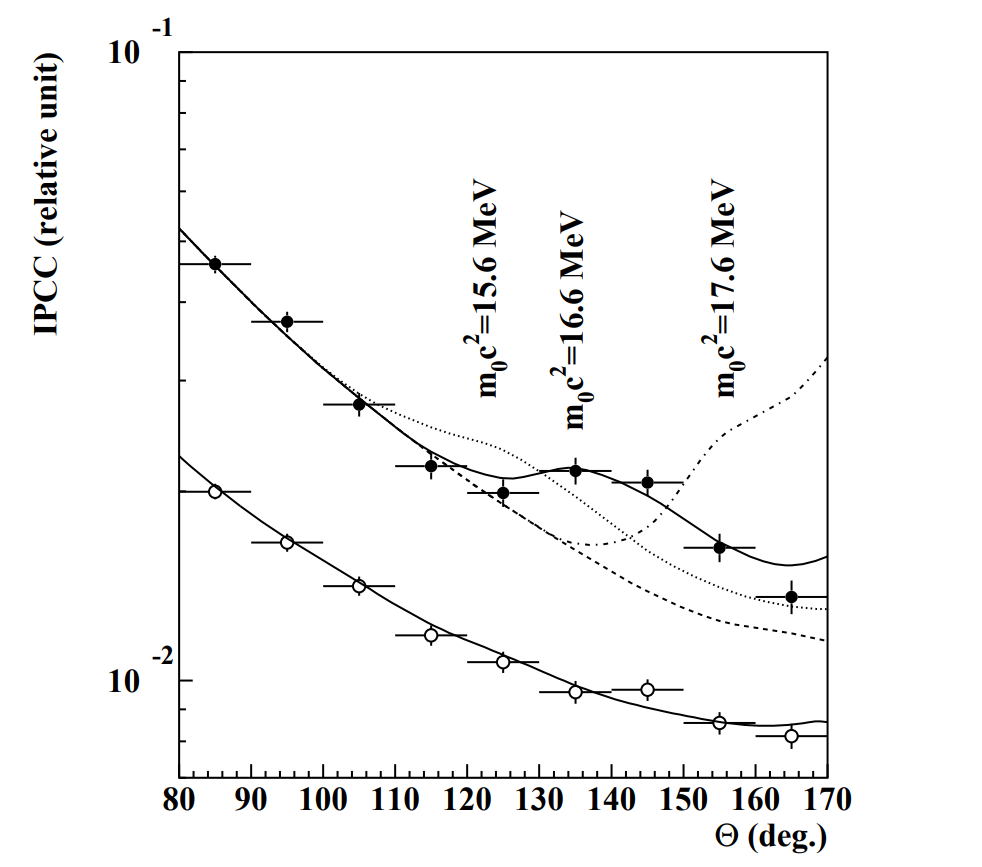
\includegraphics[width=\textwidth]{atomki_be.png}
						\caption{Experimental $e^+e^-$ pair correlations measured in the \iso{Li}{7}$(p,e^+e^-)$\iso{Be}{8} reaction with $|y| \leq 0.5$ (closed circles) and $|y| \geq 0.5$ (open circles)~\cite{atomki_be}.}
						\label{fig:atomki_be}
					\end{subfigure}
					\hfill
					\begin{subfigure}[t]{0.42\textwidth}
						\centering
						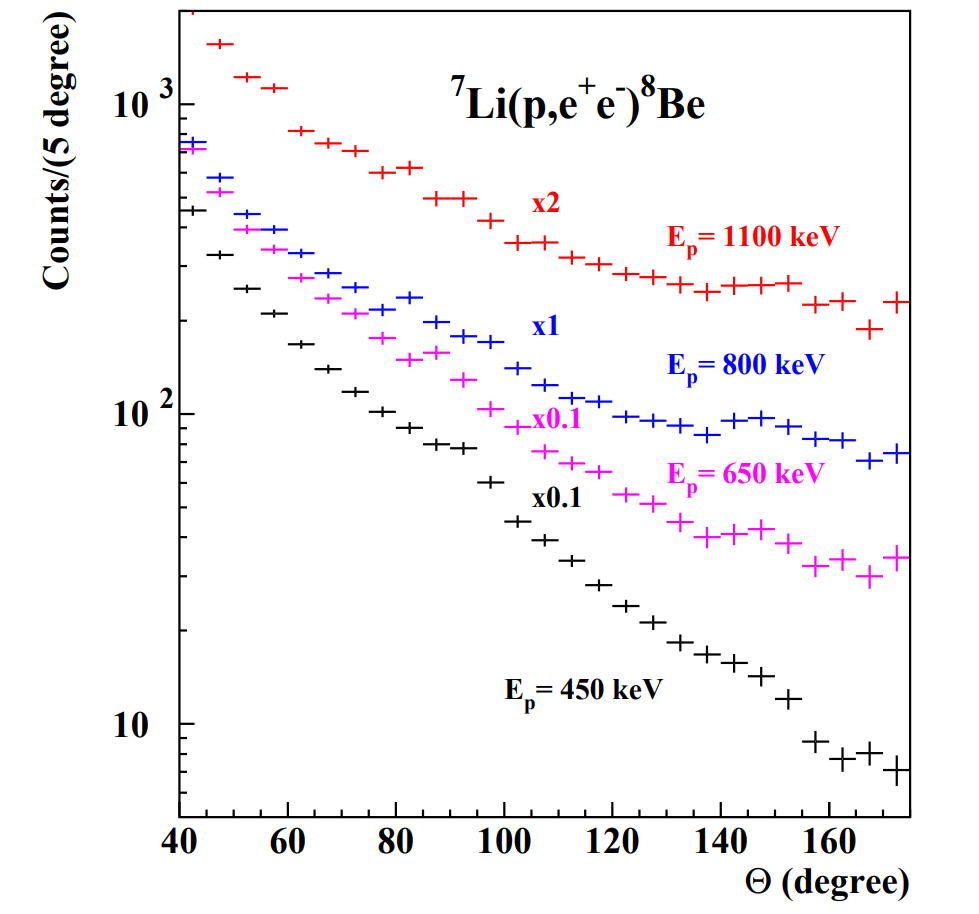
\includegraphics[width=\textwidth]{atomki_be2.png}
						\caption{Experimental $e^+e^-$ pair correlations measured in the \iso{Li}{7}$(p,e^+e^-)$\iso{Be}{8} reaction with the improved setup for different proton beam energies~\cite{atomki_be2}.}
						\label{fig:atomki_be2}
					\end{subfigure}
					\begin{subfigure}[t]{0.45\textwidth}
						\centering
						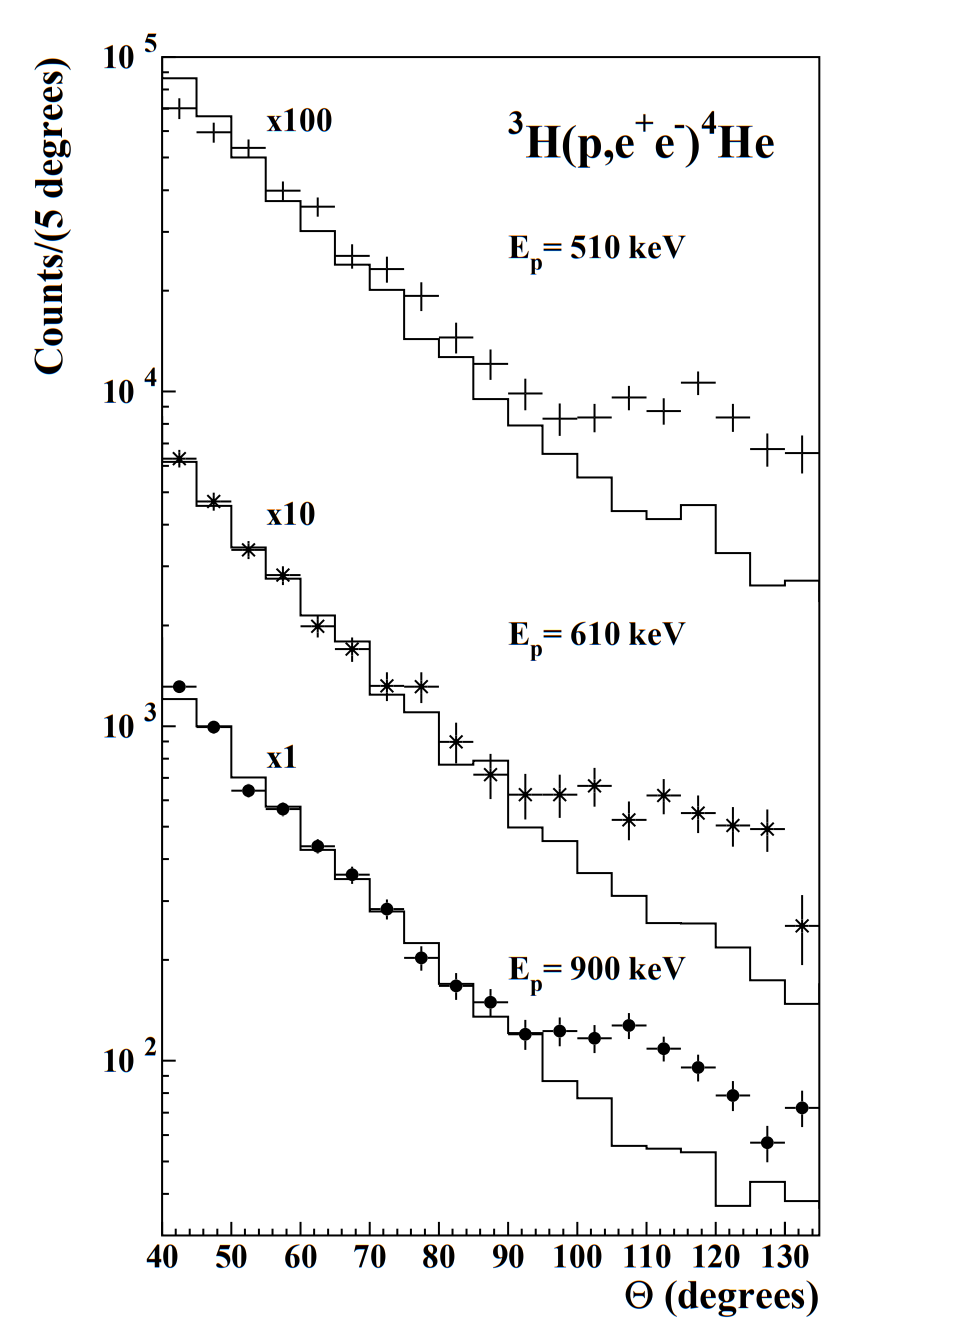
\includegraphics[width=\textwidth]{atomki_he.png}
						\caption{Experimental $e^+e^-$ pair correlations measured in the \iso{H}{3}$(p,e^+e^-)$\iso{He}{4} reaction with $|y| \leq 0.3$ for different proton beam energies~\cite{atomki_he2}.}
						\label{fig:atomki_he}
					\end{subfigure}
					\hfill
					\begin{subfigure}[t]{0.45\textwidth}
						\centering
						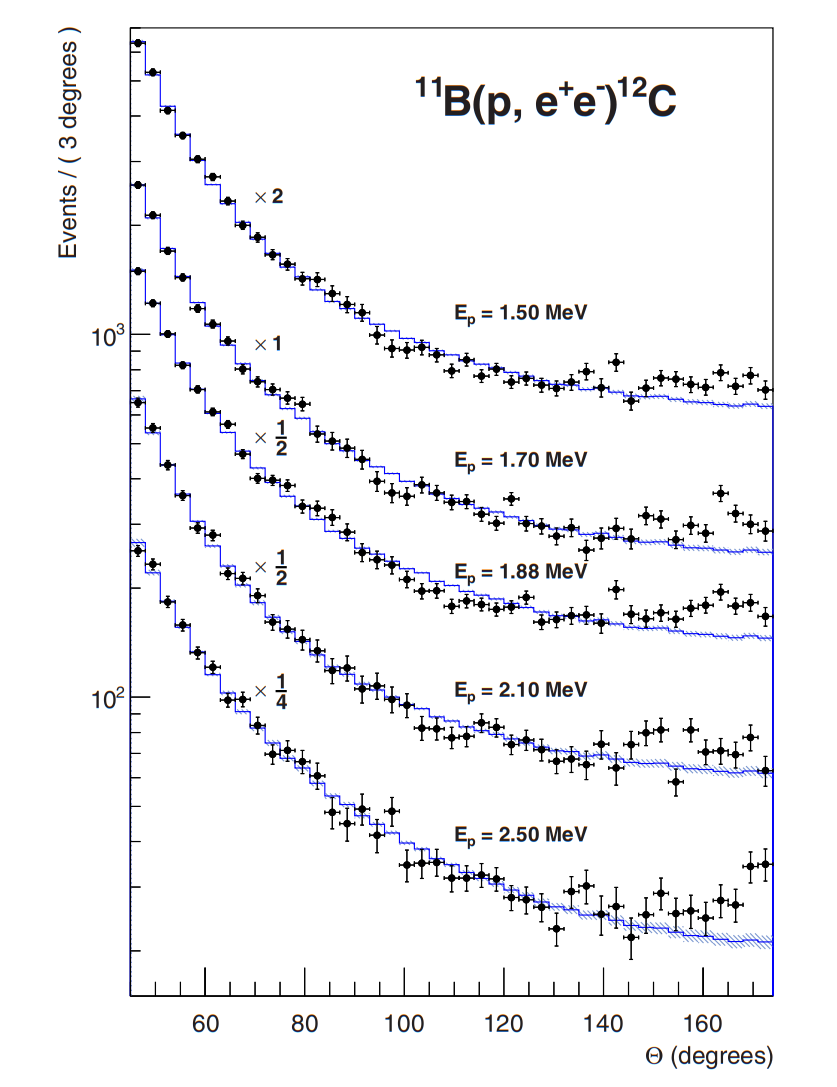
\includegraphics[width=\textwidth]{atomki_c.png}
						\caption{Experimental $e^+e^-$ pair correlations measured in the \iso{B}{11}$(p,e^+e^-)$\iso{C}{12} reaction for different proton beam energies~\cite{atomki_c}.}
						\label{fig:atomki_c}
					\end{subfigure}
					\caption{The ATOMKI anomalous \ac{IPC} measured for different nuclei.}
					\label{fig:atomki}
				\end{figure}
			
				Possible explanations of the anomaly include experimental effects, higher order processes in the Standard Model~\cite{kalman,aleksejevs} or even a~protophobic fifth force mediated by a~new \qty{17}{\MeV} boson X17~\cite{feng}.
		\subsection{Other Experiments}
			Since the ATOMKI measurements, several experiments have been initiated to attempt to replicate the results and search for the hypothetical X17 particle. The following experiments have already produced results~\cite{atomki_review}.
			
			\subsubsection{Two-arm $e^+e^-$ spectrometer in Hanoi}
				The anomaly in \iso{Be}{8} has been observed with a~high ($>4\sigma$) confidence by a~team at the Hanoi University of Sciences for $E_p = \qty{1225}{\keV}$~\cite{hanoi}. They built a~two\nobreakdash-arm spectrometer in collaboration with ATOMKI and calibrated it using the \qty{17.6}{\MeV} M1 transition. The results are shown in \cref{fig:hanoi}.
				
				\begin{figure}
					\centering
					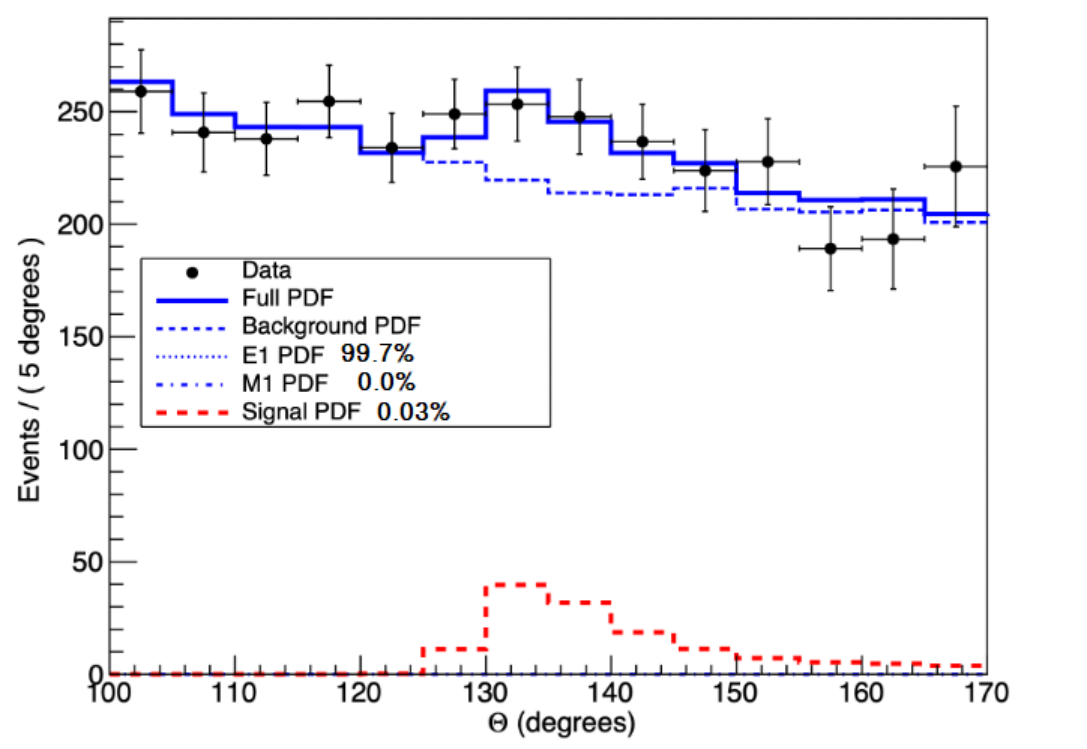
\includegraphics[width=0.75\textwidth]{hanoi.png}
					\caption{Results from the Hanoi spectrometer - angular $e^+e^-$ pair correlations measured in the \iso{Li}{7}$(p,e^+e^-)$\iso{Be}{8} reaction at $E_p = \qty{1225}{\keV}$~\cite{hanoi}.}
					\label{fig:hanoi}
				\end{figure}
			
			\subsubsection{Collisions at Nuclotron in Dubna}
				At the Joint Institute for Nuclear Research in Dubna, signal in the form of enhanced structures in the $\gamma\gamma$ spectra at \textapprox17 and \textapprox38~MeV invariant masses for $p+\mathrm{C}$, $d+\mathrm{C}$ and $d+\mathrm{Cu}$ reactions at momenta 5.5, 2.75, and 3.83~GeV per nucleon~\cite{dubna}. Monte Carlo simulations support the conclusion that the signals are a~consequence of a~decay of unknown particles X17 and E38.
				
			\subsubsection{The MEG II (Muon Electron Gamma) experiment}
				Experiments using the \iso{Li}{7}$(p,e^+e^-)$\iso{Be}{8} reaction were carried out at the Paul Scherrer Institute with the MEG II superconducting solenoid spectrometer~\cite{megii}. Analysis of the data with $E_p = 1080$~keV exciting both of the resonances (beam fully stopping in the target) found no significant evidence supporting the X17 hypothesis, results are shown in \cref{fig:megii}. An upper bound (at 90\% confidence) on the X17\nobreakdash-to\nobreakdash-$\gamma$ branching ratio was set at $1.2\cdot10^{-5}$ for the 18.15~MeV state (larger than the ratio $5.8\cdot10^{-6}$ obtained by ATOMKI in 2016).
				
				\begin{figure}
					\centering
					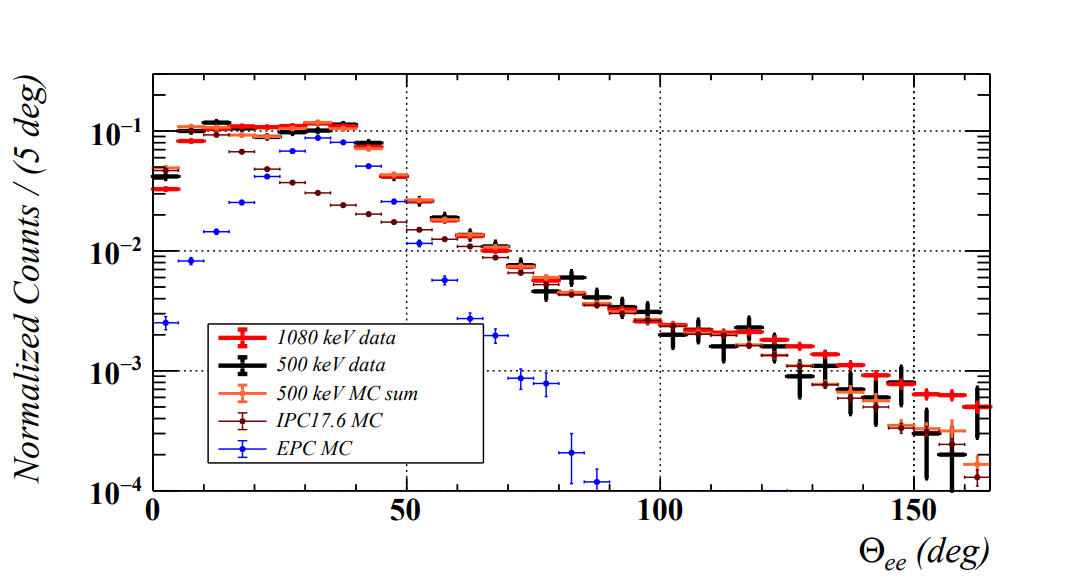
\includegraphics[width=0.9\textwidth]{megii.png}
					\caption{Results from the MEG II experiments -- angular correlation of $e^+e^-$ pairs with $E_\text{sum} \in [16,20]$~MeV measured in the \iso{Li}{7}$(p,e^+e^-)$\iso{Be}{8} reaction with proton beam energies 500 and 1080~keV. The 500~keV dataset is fitted with Monte Carlo of both the \ac{IPC} deexcitation and the \ac{EPC} produced by gammas~\cite{megii}.}
					\label{fig:megii}
				\end{figure}
			
	
	\section{X17 Project at IEAP CTU}
	\label{sec:IEAP}
		The aim of the X17 project at the Van der Graaff facility of the \acl{IEAPCTU} is to reproduce the results of the original ATOMKI experiments with \iso{Li}{7} and \iso{H}{3} targets using an independent $e^+e^-$ spectrometer. In order to effectively measure the anomaly, we need to reconstruct both the energy and the angular correlation of the $e^+e^-$ pairs. The spectrometer will use three layers of detectors to achieve this -- \acf{TPX3} silicon pixel detector and \acf{MWPC} layers for the angle reconstruction and a~\acf{TPC} layer for the energy reconstruction. The schematics of the prepared detector is in \cref{fig:ieap}.
			
			\begin{figure}
				\centering
				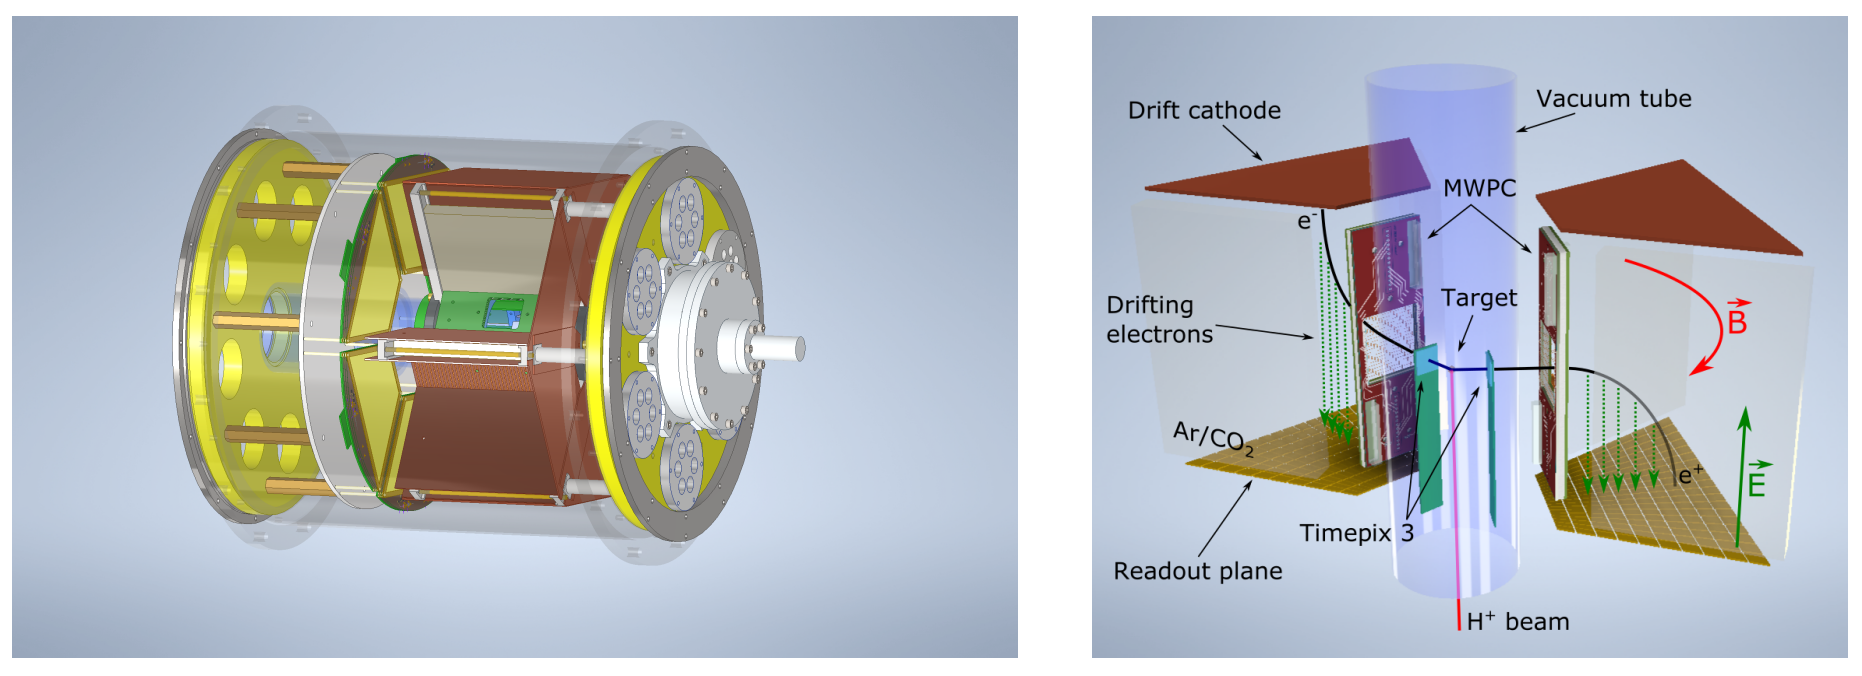
\includegraphics[width=\textwidth]{ieap_x17.png}
				\caption{Schematics of the detector at the Van der Graaff facility at~\ac{IEAPCTU}~\cite{x17_utef}.}
				\label{fig:ieap}
			\end{figure}
		
		The energy of $e^+e^-$ pair produced in the reaction is given by the energy available $E_\text{r}$ in the reaction and can be distributed between them arbitrarily. Nonetheless in the decay of the hypothetical X17 particle, electron and positron should have similar energy and we can therefore use a~cut $|y| \leq 0.5$ in the disparity parameter (defined in \cref{eq:dispar}). Interesting events should rarely have a~particle with an energy below $E_\text{r}/4$ (roughly \qty{4}{\MeV}). Electrons with such low energies are scattered significantly by even a~thin layer of relatively light material, for this reason the \ac{TPX3} layer will be inside of the vacuum tube and the tube will have a~thinned aluminum segment or Kapton\texttrademark\ windows.
		
		\ac{TPX3} can measure (in each \qtyproduct{55x55}{\um} pixel of its \numproduct{256x256} grid) \ac{ToA} with \qty{1.6}{\ns} precision and \ac{ToT} which reflects the deposited energy. This potentially allows 3D~tracking if we increase the chip thickness at the cost of increased scattering. The layer can reconstruct the reaction vertex and the angular correlation with high precision. Preparatory studies of the angular correlation reconstruction~\cite{triangle}, and energy deposition in the sensor~\cite{tpx3_tracks} have been made.
		
		The layer of \acp{MWPC} with sensitive area \qtyproduct{40x38}{\mm} will be outside of the beam pipe. It will provide an extra point on the particle trajectory which can help with the estimation of the reaction vertex and improve the \ac{TPC} performance by providing its entry point.
		
		The \acp{TPC} that are the subject of this thesis, are in a~magnetic field generated by permanent magnets positioned between them and provide 3D track reconstruction and subsequent momentum and particle identification (its charge, or even type based on its stopping power). They avoid radiative losses thanks to the low density and atomic number of the gas mixture. For the readout, triple \ac{GEM} will be used. The magnetic field layout in our \acp{TPC} is atypical -- orthogonal to the electric field inside the chamber, this is why we call them \acf{OFTPC}. Further details about our \acp{OFTPC} are provided in \cref{sec:oftpc}.
	\chapter{Time Projection Chamber}
\label{sec:tpc}
	A~\acf{TPC} is a~gaseous detector that uses the drift times of ionization electrons produced by a~charged particle in an (ideally uniform) electric field to reconstruct the particle's 3D~trajectory. The 2D~projection is measured by an amplification stage at the end of the drift volume. When placed inside a~magnetic field (typically parallel to the electric field), the momentum of the incident particle can be inferred from the curvature of its trajectory. Particle identification is also possible using the ionization energy loss inside the \ac{TPC} (see \cref{fig:particleid}). The following text (including \cref{sec:transport,sec:readout}) is based primarily on the reviews by Hilke~\cite{TPCs} and the Particle Data Group~\cite{pdg2024}.
	
	\begin{figure}[H]
		\centering
		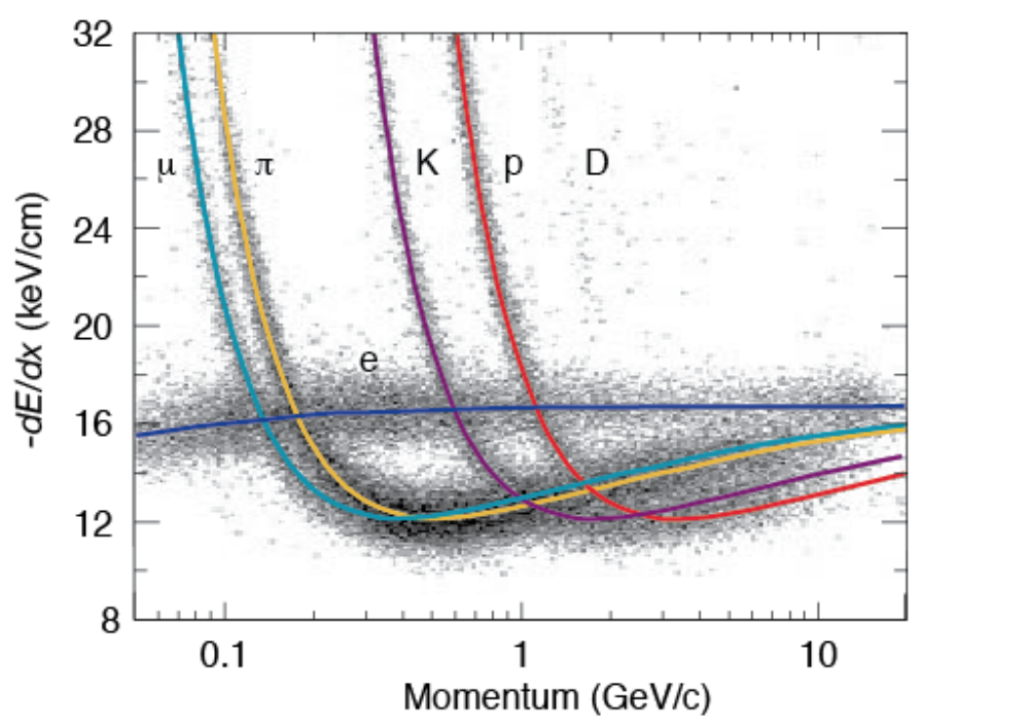
\includegraphics[width=0.6\textwidth]{particle_id.png}
		\caption{Particle identification in the PEP-4 \ac{TPC} at SLAC based on the energy loss per distance $\dv{E}{x}$ in the 80:20 Ar:CH$_4$ filling at \qty{8.5}{atm} pressure~\cite{pid_og,particleid}.}
		\label{fig:particleid}
	\end{figure}
	
	Large \acp{TPC} are sensitive to small distortions in the electric field (imperfections in the field cage, accumulation of positive ions in the gas volume) and to $\mathbf{E}\cross\mathbf{B}$ effects on the drift velocity (see \cref{eq:drift} below). Diffusion of the drifting electrons deteriorates the spatial resolution significantly, but it can be reduced up to \textapprox10~times by a~strong $\mathbf{B}\parallel\mathbf{E}$ field (see \cref{eq:difmag}).
	
	In neutrino and other rare-event experiments, large (up to 600 tons) \acp{LArTPC} are used for particle identification and calorimetry. The ionization electrons can be drifted for many meters with small diffusion. Scintillation photons are also measured.
	
	\section{Charge transport in gases}
	\label{sec:transport}
		When a~charged particle crosses the volume of a~\ac{TPC}, it loses energy by excitation and ionization of the detector gas\footnote{A minimum ionizing particle loses on the order of \unit{\keV} per centimeter traveled at \qty{1}{atm} pressure.}. Most ionizing collisions produce a~single ionization electron, sometimes a~few electrons of secondary ionization are produced near the collision vertex, creating a~cluster. In rare cases, the ionization electron has energy large enough to create a~measurable track; such an electron is called a~$\delta$\nobreakdash-electron.
		
		After their release, the ionization electrons are separated from positive ions by the electric field, and they both drift and diffuse in opposite directions towards the electrodes. The charges are accelerated by the electric field inside the chamber, and they lose speed by colliding with the gas particles, quickly reaching a~constant (for a~given field $\mathbf{E}, \mathbf{B}$) mean drift velocity. The electrons can be absorbed by electronegative impurities, such as halides, O$_2$, and H$_2$O.
		
		In mixtures with a~noble gas component, if the excitation energy of the noble gas is higher than the ionization potential of an admixture, more free electrons can be produced through collisions of the gas particles (so\nobreakdash-called Penning transfer) and through absorption of emitted photons.
		
		If the electric field is strong enough, the electrons can cause further ionization and excitation of the gas, leading to the development of a~Townsend avalanche~\cite{Townsend1900}.
	
		\subsection{Drift}			
			In many gases (called "hot", e.g., Ar or CH$_4$), the drift velocity is much greater than that of their thermal motion thanks to a~high proportion of elastic collisions. On the other hand, "cold" gases like CO$_2$ have a~higher proportion of inelastic collisions (e.g., due to the excitation of rotational and vibrational states) and therefore much lower drift velocity\footnote{It is not always so simple; sometimes, when the electrons are slowed down by inelastic collisions, they reach a~minimal cross-section for elastic collisions (so-called Ramsauer-Townsend effect), making them drift faster, due to a~less chaotic motion.}.
			
			The ions produced by the ionization lose a~significant portion of their energy during each collision since their mass is close to the mass of the gas particles\footnote{Average energy loss of ions with mass $m_i$ during collision with mass $M$ is $\Delta E = \frac{2m_i M}{(m_i+M)^2}$.}. This, together with their large collision cross section, makes their drift velocity much smaller (about three orders of magnitude), and their energy is close to thermal.
			
			The drift is also influenced by the magnetic field. Langevin derived a~good approximation for the drift velocity vector:
				\begin{equation}
					\label{eq:drift}
					\mathbf{v}_\text{d} = \left(\frac{\mathbf{E}}{\norm{\mathbf{E}}} + \omega\tau\frac{\mathbf{E}\times\mathbf{B}}{\norm{\mathbf{E}}\norm{\mathbf{B}}} + \omega^2\tau^2\frac{\mathbf{E}\cdot\mathbf{B}}{\norm{\mathbf{E}}\norm{\mathbf{B}}}\cdot \frac{\mathbf{B}}{\norm{\mathbf{B}}}\right) \frac{q\tau}{m(1+\omega^2\tau^2)}\norm{\mathbf{E}},
				\end{equation}
			where $q$ is the charge of the particle, $m$ is its mass, $\tau$ is the mean time between collisions, and $\omega = \frac{q}{m}\norm{\mathbf{B}}$ is the Larmor frequency. For orthogonal fields $\mathbf{E}\perp\mathbf{B}$, it can be shown that the magnetic field bends the direction of the drift by the so\nobreakdash-called Lorentz angle:
				\begin{equation}
					\label{eq:lorentz}
					\tan\psi = -\omega\tau.
				\end{equation}
			The drift of ions is only negligibly influenced by the magnetic field ($\omega\tau\sim10^{-4}$ is small due to the low drift velocity). In a~standard \ac{TPC}, $\mathbf{E}$ is parallel to $\mathbf{B}$ and the influence of the magnetic field on the drift is minimal. Without magnetic field, we can write
				\begin{equation}
					\mathbf{v}_\text{d} = \frac{q\tau}{m} \mathbf{E} = \mu \mathbf{E},
				\end{equation}
			where $\mu$ is called charge mobility.
			
		\subsection{Diffusion}
			Due to collisions, a~cloud of electrons or ions originating from the same point will show a~Gaussian density distribution at time $t$ while drifting in the electric field $\mathbf{E} = (0,0,E_z)$ along the $z$\nobreakdash-coordinate:
				\begin{equation}
					\rho(x,y,z,t) = (4\pi Dt)^{-\frac{3}{2}} \exp\left(-\frac{x^2+y^2+(z-v_\text{d}t)^2}{4Dt}\right),
				\end{equation}
			where the diffusion coefficient $D$ can be expressed as
				\begin{equation}
					D = \frac{\lambda^2}{3\tau} = \frac{\lambda v_\text{d}}{3} = \frac{v_\text{d}^2\tau}{3} = \frac{2\varepsilon\tau}{3m},
				\end{equation}
			where $\lambda$ is the mean free path and $\varepsilon$ the mean kinetic energy. The lateral diffusion width~$\sigma_x$ after a~drift distance~$L$ can be expressed as
				\begin{equation}
					\sigma_x^2 = 2Dt = \frac{4\varepsilon L}{3qE_z}.
				\end{equation}
			The minimal diffusion width is given by the lowest possible energy of the particles $\varepsilon_\text{th} = \frac{3}{2}kT$ (corresponding to the thermal motion):
				\begin{equation}
					\sigma_{x, \,\text{min}}^2 = \frac{2kTL}{qE}.
				\end{equation}
			For electrons in "cold gases" (e.g., Ar/CO$_2$ mixture), the diffusion approaches this limit up to a~certain field intensity (\textapprox\qty{100}{\V\per\cm} at \qty{1}{atm} pressure)\footnote{In our detector with 70:30 Ar:CO$_2$ mixture, the maximal drift distance is $L=\qty{16}{\cm}$, $E=\qty{400}{\V\per\cm}$, and therefore $\sigma_{x, \,\text{min}} = \qty{0.45}{\mm}$, quite close to the actual diffusion \textapprox\qty{1}{\mm} seen in the simulation of the map in \cref{sec:map}.}. In reality, the transversal diffusion of electrons can differ significantly from their longitudinal diffusion, and simulations are necessary to get a~precise result. Ions do not change their direction between collisions significantly, and their diffusion is therefore much smaller.
			
			In most \acp{TPC}, the transversal (but not the longitudinal) diffusion is reduced by the magnetic field, since it is parallel to the electric field and curves the diffusing electrons around their mean trajectory:
				\begin{equation}
					\label{eq:difmag}
					\frac{D_\text{T}(B)}{D_\text{T}(0)} = \frac{1}{C+\omega^2\tau_2^2},
				\end{equation}
			where $C$ and $\tau_2$ are parameters dependent on the gas used. At low intensity of the magnetic field, we can use an approximation $C\approx1$ and $\tau_2\approx\tau$.
			
	\section{Examples of TPCs}
		\subsection{The original TPC at PEP-4 at SLAC}
			The original \ac{TPC} used in the PEP-4 experiment at SLAC in the 1980s (\cref{fig:pep4}) was a~\qtyproduct[product-units=repeat]{2x2}{\m} hollow cylinder with a~central cathode that produced a~strong electric field \qty{750}{\V\per\cm}, making the ionization electrons drift towards one of the endcaps~\cite{pep4-2}. It was filled with an~80:20 Ar:CH$_4$ mixture at \qty{8.5}{atm} pressure and placed inside a~\qty{0.4}{\tesla} solenoidal magnetic field.
			
			The readout consisted of \acp{MWPC}, where electrons are accelerated towards the anode wires fast enough to further ionize the gas and cause an avalanche (details are provided in \cref{sec:MWPC}). The wires had radial spacing \qty{4}{\mm}, and fifteen of the sense wires had the cathode segmented into \qtyproduct{7.0x7.5}{\mm} pads \qty{4}{\mm} under them (\cref{fig:pep4} right). When collecting electrons on the anode wire, signal is induced on the nearest \numrange{2}{3} cathode pads.
			
			\begin{figure}
				\centering
				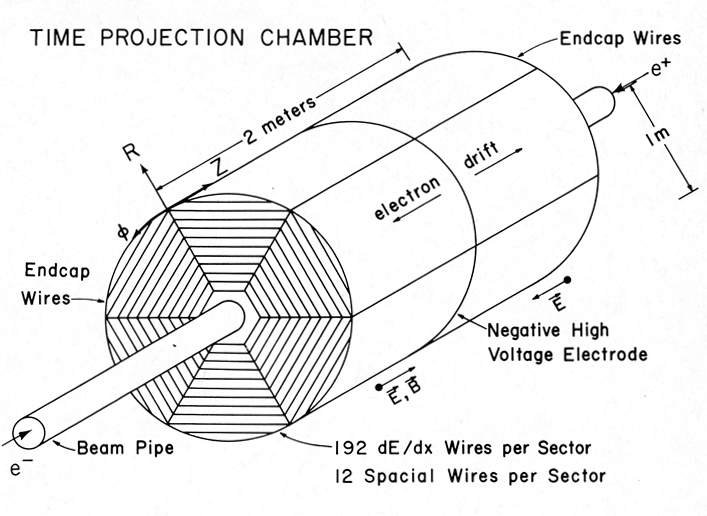
\includegraphics[width=0.6\textwidth]{pep4_tpc.png}
				\hfill
				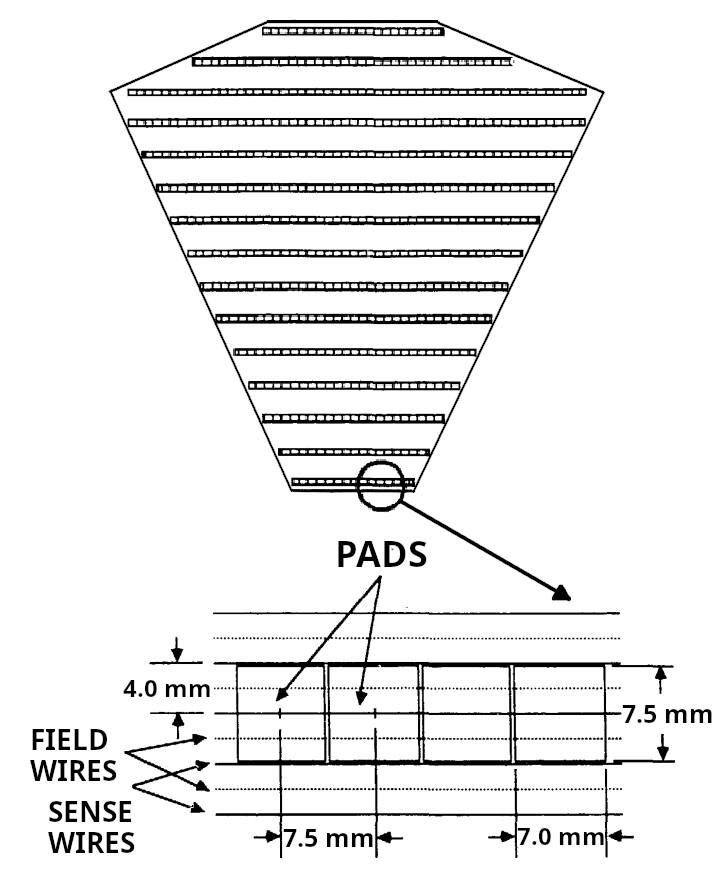
\includegraphics[width=0.38\textwidth]{pep4_readout_edit.png}
				\caption{Schematic view of the PEP-4 \ac{TPC}~\cite{pep4}. A~charged particle produced in a~collision in the beam pipe creates a~spiral ionization track in the magnetic field. The central cathode then accelerates ionization electrons towards the endcap anode wires where they are multiplied and read out. A~\ac{TPC} sector with a~detailed view of one of the pad rows is shown on the right~\cite{pep4_readout}.}
				\label{fig:pep4}
			\end{figure}
		
		\subsection{ALICE TPC}
			The ALICE \ac{TPC} (\cref{fig:alice}) is the main detector used for charged particle tracking and recognition in collisions at the ALICE experiment at the CERN LHC~\cite{ALICE}. Similarly to PEP\nobreakdash-4, it is a~hollow cylinder with outer radius \qty{2.5}{\m} and height \qty{5}{\m}. It is placed in a~\qty{0.5}{\tesla} solenoidal magnetic field, and the central cathode generates a~\qty{400}{\V\per\cm} electric field inside the field cage. The gas mixture in the detector is 90:10:5 Ne:CO$_2$:N$_2$ (molar fraction), mainly chosen for its higher ion mobility compared to Ar mixtures. In 2020, the readout of the \ac{TPC} was upgraded from \acp{MWPC} to stacks of four \ac{GEM} foils (principle described in \cref{sec:mpgd}). This allows reading events continuously at a~higher rate.
			
			\begin{figure}
				\centering
				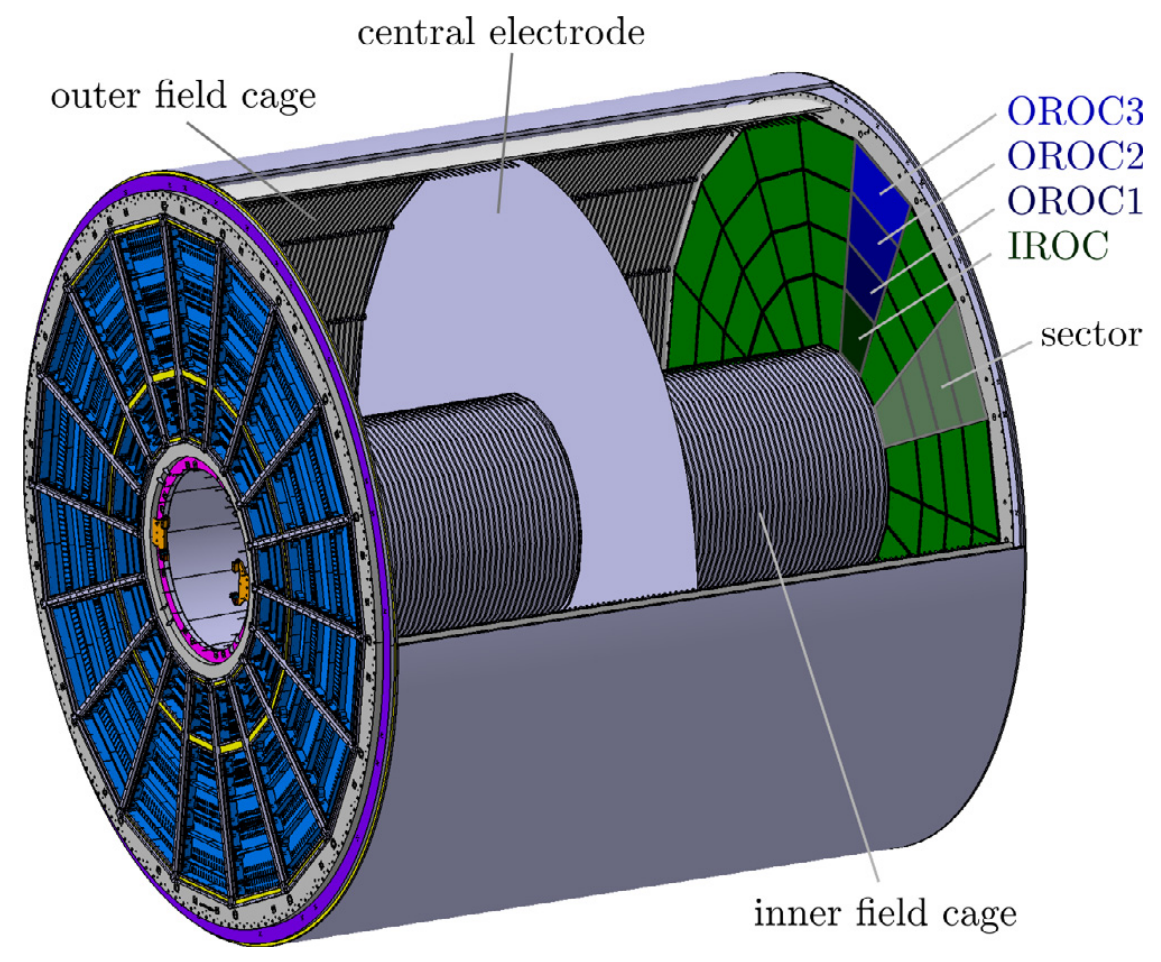
\includegraphics[width=0.65\textwidth]{alice_tpc.png}
				\hfill
				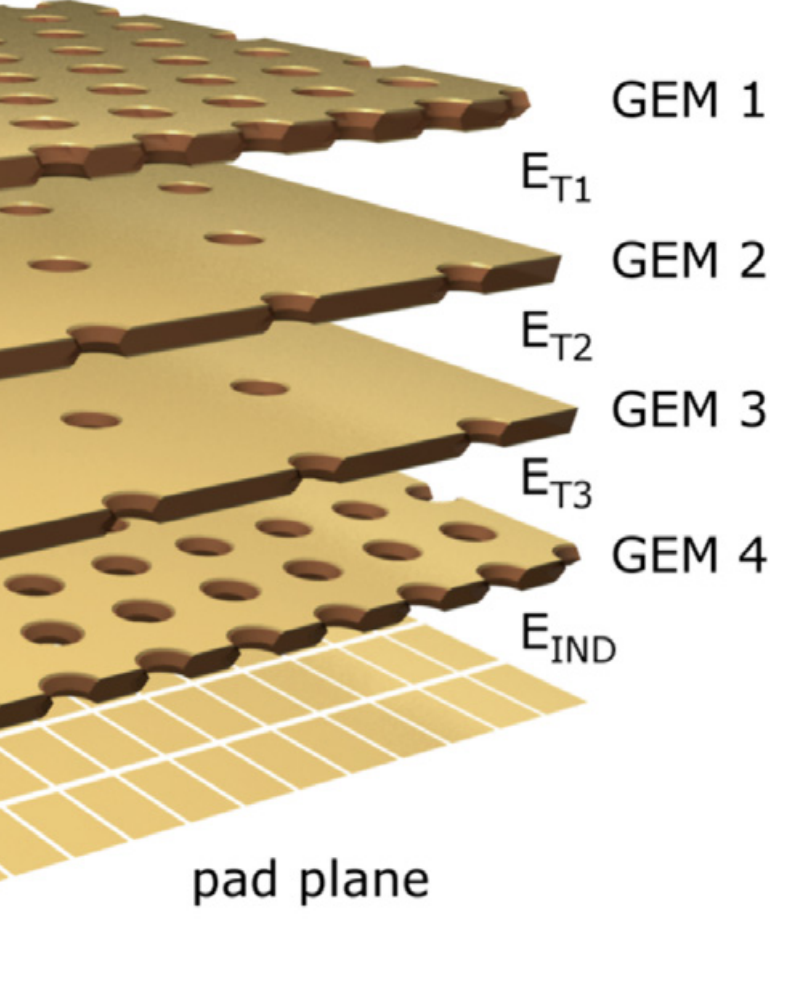
\includegraphics[width=0.33\textwidth]{alice_gem.png}
				\caption{Schematic view of the ALICE \ac{TPC}~\cite{ALICE_upgrade2}. The readout at each endcap is divided into 18 sectors, each subdivided into an Inner Readout Chamber (IROC) with one \ac{GEM} stack and Outer Readout Chamber (OROC) with three \ac{GEM} stacks. A~visualization of a~\ac{GEM} stack is on the right~\cite{ALICE_gem}.}
				\label{fig:alice}
			\end{figure}
			
		\subsection{CERES/NA45 radial-drift TPC}
			In 1998, the CERES/NA45 (Cherenkov Ring Electron Spectrometer) experiment (\cref{fig:ceres}) at the CERN SPS was upgraded with the first \acf{rTPC} to achieve a~higher momentum resolution~\cite{ceres}. Unlike a~standard \ac{TPC}, the electric field \qtyrange{600}{200}{\V\per\cm} was arranged radially with the magnetic field (inhomogeneous, up to \qty{0.5}{\tesla}) by two solenoidal coils with opposite polarity. The outward drift of the ionization electrons is affected by the crossing fields as shown in \cref{eq:drift} and the drift velocity is not uniform due to the varying electric field. The \ac{rTPC} was filled with an 80:20 Ne:CO$_2$ gas mixture, which has relatively small diffusion coefficients and Lorentz angle. The readout was handled by conventional \acp{MWPC} (\cref{fig:ceres_readout}).
			
			\begin{figure}
				\centering
				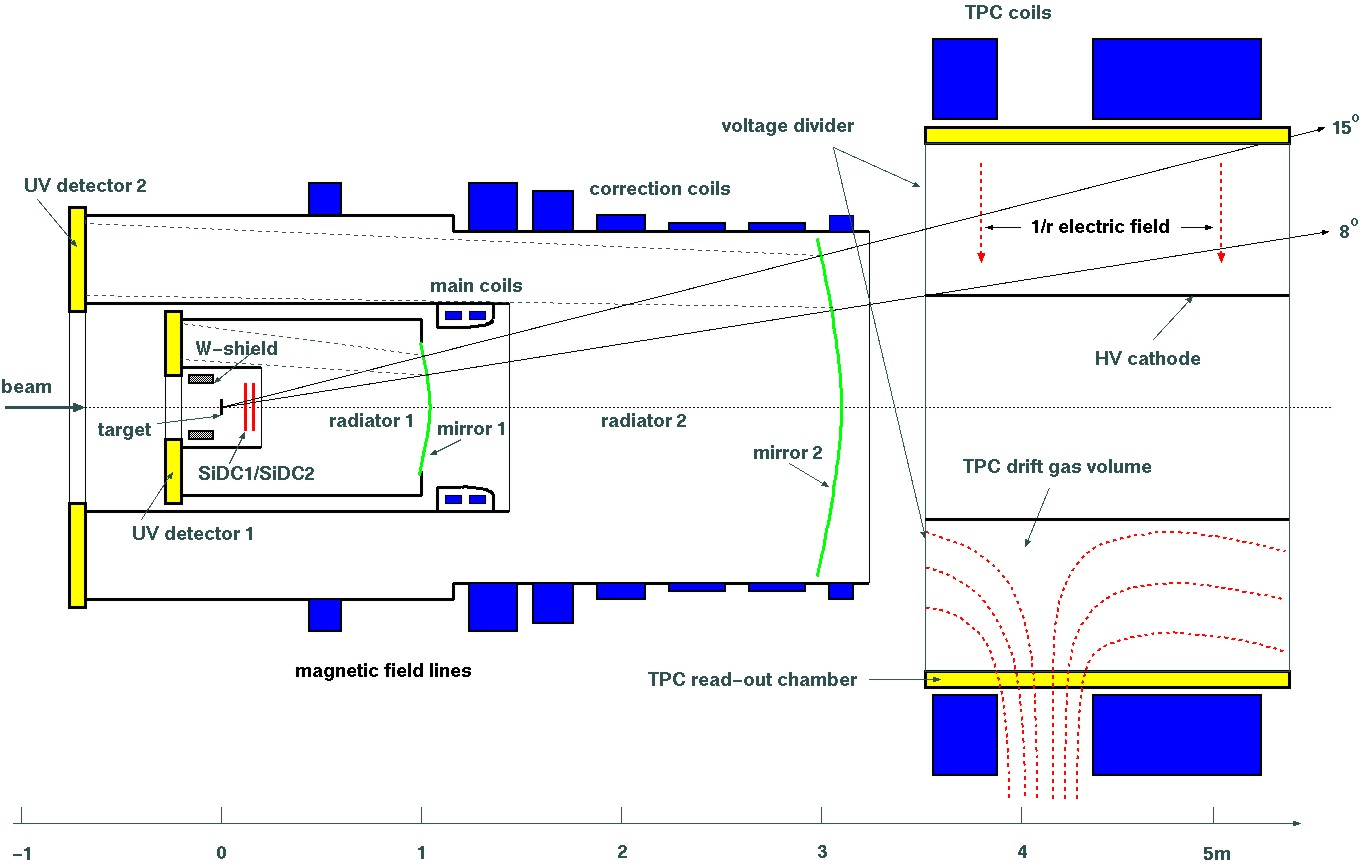
\includegraphics[width = \textwidth]{ceres.jpg}
				\caption{Experimental setup of the CERES/NA45 experiment with two \acfp{RICH} on the left and a~\ac{rTPC} on the right. The magnetic field (red) is generated by two solenoidal coils (blue) with opposite polarity. Produced ionization electrons drift outward radially towards the readout chamber (yellow)~\cite{ceres}.}
				\label{fig:ceres}
			\end{figure}
			\begin{figure}
				\centering
				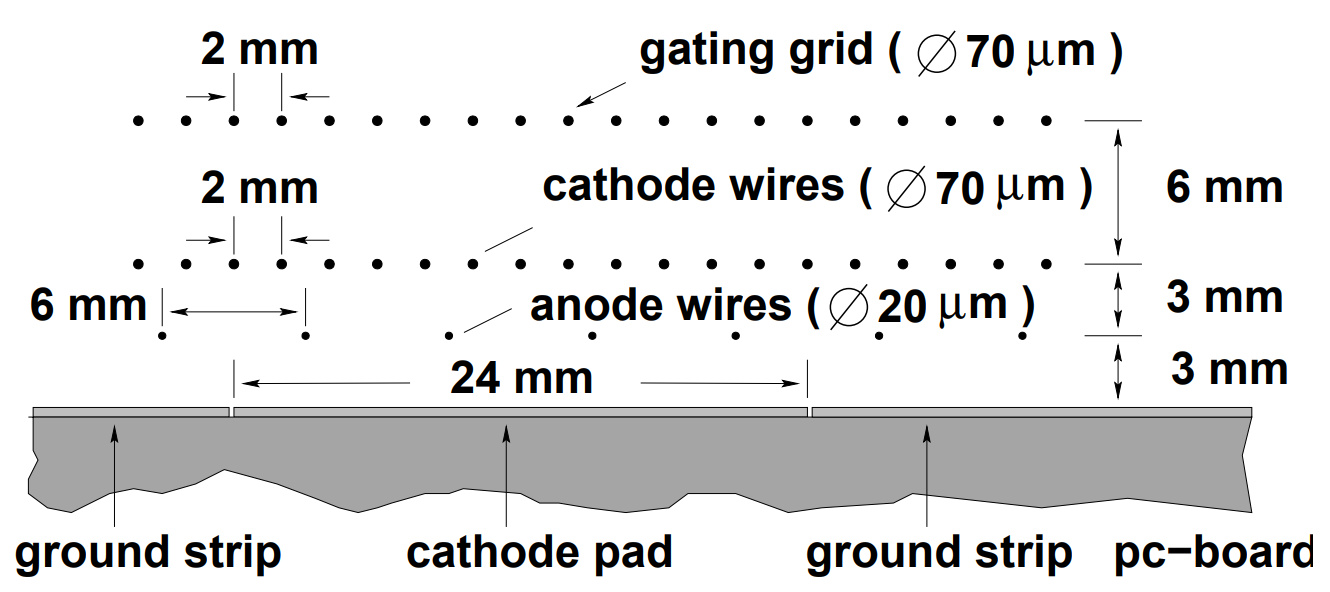
\includegraphics[width=0.7\textwidth]{ceres_readout.png}
				\caption{Cross section of a~CERES/NA45 readout \ac{MWPC}. The wires are stretched in the azimuthal direction above the pad plane. The gating grid controls the passage of electrons and ions~\cite{ceres}.}
				\label{fig:ceres_readout}
			\end{figure}
			
			The field configuration in an \ac{rTPC} enables a~larger number of pads compared to a~standard \ac{TPC}, leading to improved spatial resolution and possibility of larger multiplicity rates. Since the drift time is lower, the detector is faster.
			
			After developing the algorithm described in this thesis for our \acp{OFTPC} at \ac{IEAPCTU}, we noticed the similarities with the approach used by the CE\-RES/NA45 \ac{rTPC}, when accounting for the transport process of charged clusters in the complex fields. The detector hit coordinates (pad, time, and plane) were transformed using look\nobreakdash-up tables. The tables were calculated using a~Runge-Kutta method to integrate the Langevin approximation of the drift velocity (\cref{eq:drift}). The drift velocity in the radial field was calibrated using seven parallel laser rays. This calibration was then used to correct compared to the Magboltz Monte Carlo drift~\cite{magboltz}. Measured mobility differed significantly from a~Magboltz simulation. The tracks were fitted using reference tables with hit coordinates of tracks simulated with GEANT Monte Carlo.
			
		\subsection{Other interesting radial-drift TPCs}
			After CERES/NA45, several experiments adopted similar field layout for their \acp{TPC}. Here, we briefly describe \acs{BONuS12} and \acs{ALPHA}\nobreakdash-g \acsp{rTPC}. Other noteworthy experiments are \ac{muEDM} at the Paul Scherrer Institute~\cite{muEDM}, and the Solenoidal Tracker (STAR) at \ac{RHIC} featuring a~\ac{FTPC}~\cite{STAR}.
			\subsubsection{BONuS12 rTPC}
				In 2020, the \acf{BONuS12} experiment used an \ac{rTPC} (\cref{fig:bonus}) to measure low-momentum spectator protons produced in $e^- d \rightarrow e^- p_\text{s}X$ scattering~\cite{bonus}. It was filled with a~80:20 He:CO$_2$ gas mixture and placed inside a~\qty{4}{\tesla} solenoidal magnetic field, perpendicular to the radial electric field (\qty{1100}{\V\per\cm} on average), which causes a~tilt of the drift (see \cref{eq:lorentz}). The amplification stage consisted of cylindrical triple \ac{GEM} stacks.
				
				\begin{figure}
					\centering
					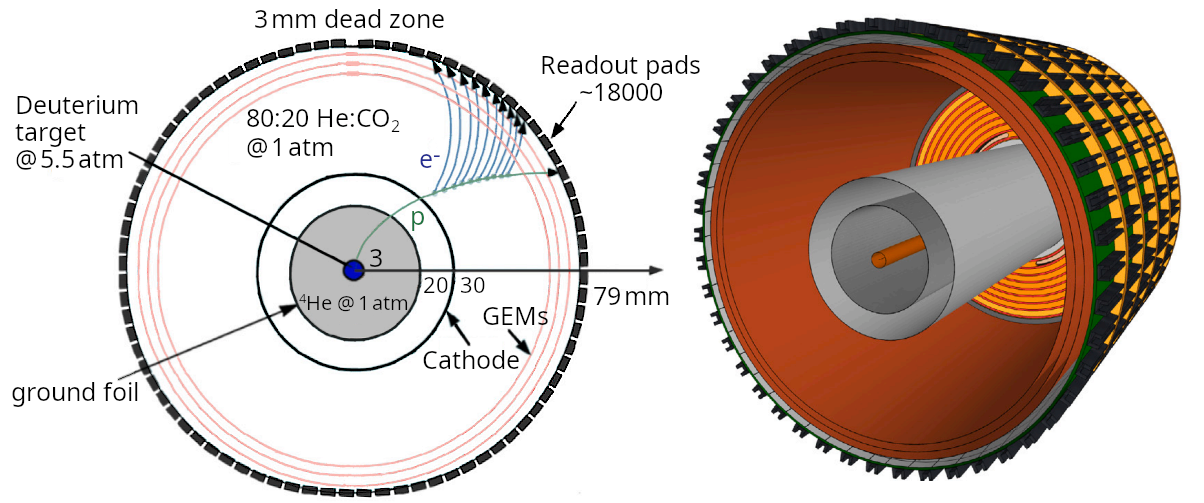
\includegraphics[width=\textwidth]{bonus12_edit.png}
					\caption{Schematic view of the \ac{BONuS12} \ac{rTPC}~\cite{bonus}.}
					\label{fig:bonus}
				\end{figure}
				
				\garfieldpp simulations and study of reconstructed tracks have shown that the radial component of the drift velocity nearly proportional to the radial electric field, and the $r$\nobreakdash-coordinate can be reconstructed using an analytical formula. Similarly, the azimuthal component is nearly proportional to the radial component, resulting in an approximately constant Lorentz angle between the radial and actual drift directions, and the $\phi$\nobreakdash-coordinate can be solved analytically. The remaining $z$\nobreakdash-coordinate stays undistorted. The momentum is determined by fitting tracks with a~helix, while accounting for the energy losses (the small variation of magnetic field along the $z$\nobreakdash-axis has a~negligible effect).
				
			\subsubsection{ALPHA-g rTPC}
				In 2023, the \acf{ALPHA} collaboration published results of measurements of antihydrogen~(\antiH) annihilation\footnote{The main \antip annihilation mode is into several $\pi^\pm$ and $\pi^0$, only the $\pi^\pm$ tracks being long enough to be reconstructed. The scattering of $\pi^\pm$ is not negligible, and photons from $\pi^0$ decay create $e^+e^-$ pairs as background.} after release from magnetic confinement, demonstrating behavior consistent with gravitational attraction to the Earth~\cite{alpha_nature}. They used a~\qty{2.3}{m} long \ac{rTPC} (\cref{fig:alpha-g}) with outer and inner diameters of \qty{40}{cm} and \qty{20}{cm}, placed in a~\qty{1}{\tesla} solenoidal magnetic field, and filled with an Ar/CO$_2$ mixture~\cite{alpha_rtpc}. The readout consists of an \ac{MWPC} (\cref{fig:alpha-g_drift}). The radial confinement of the cold~\antiH is achieved with a~superconducting octupole magnet, the axial with a~set of so\nobreakdash-called \emph{mirror} coils.
				
				\begin{figure}
					\centering
					\begin{subfigure}[t]{0.49\textwidth}
						\centering
						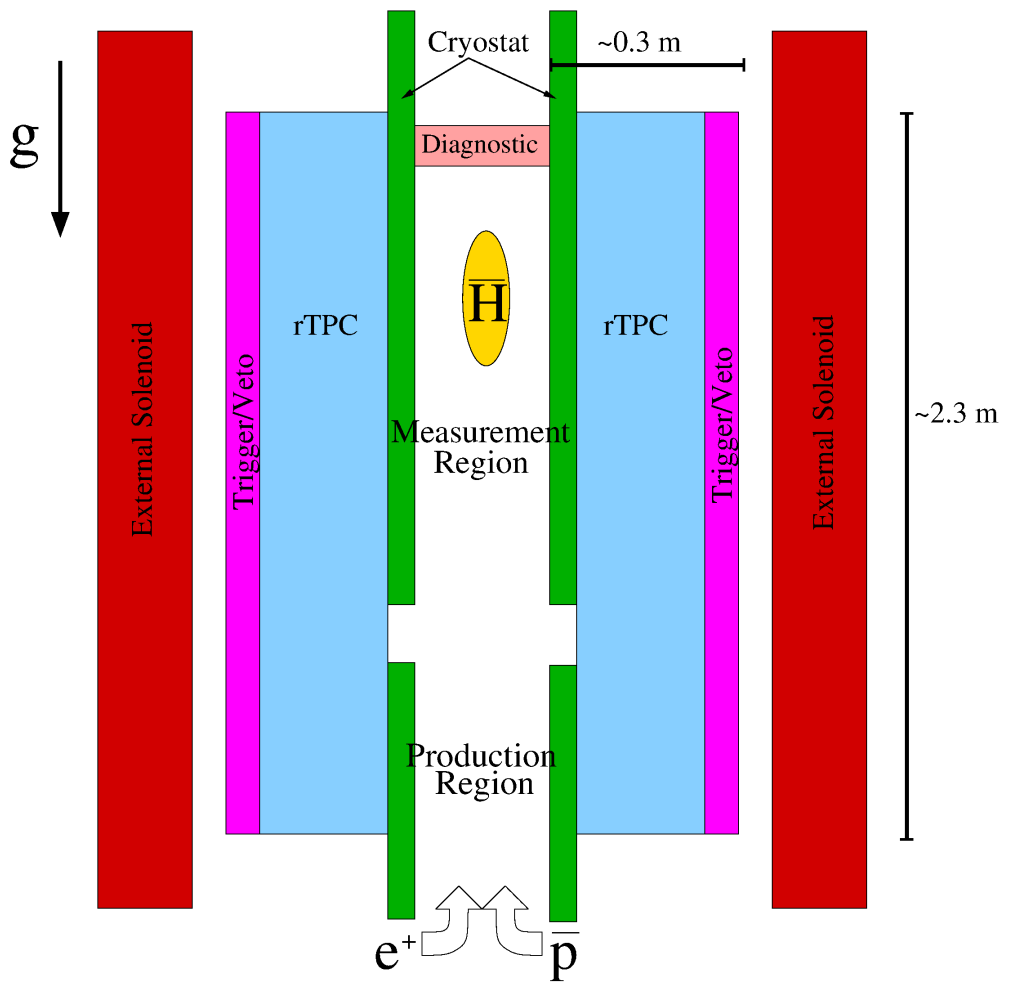
\includegraphics[width=\textwidth]{alpha-g.png}
						\caption{Sketch of \acs{ALPHA}\protect\nobreakdash-g. Antiprotons and positrons are injected from the bottom and form~\antiH in a~Penning trap while being cooled by the cryostat (green). The annihilation is reconstructed by the \ac{rTPC} (blue).}
						\label{fig:alpha-g}
					\end{subfigure}
					\hfill
					\begin{subfigure}[t]{0.49\textwidth}
						\centering
						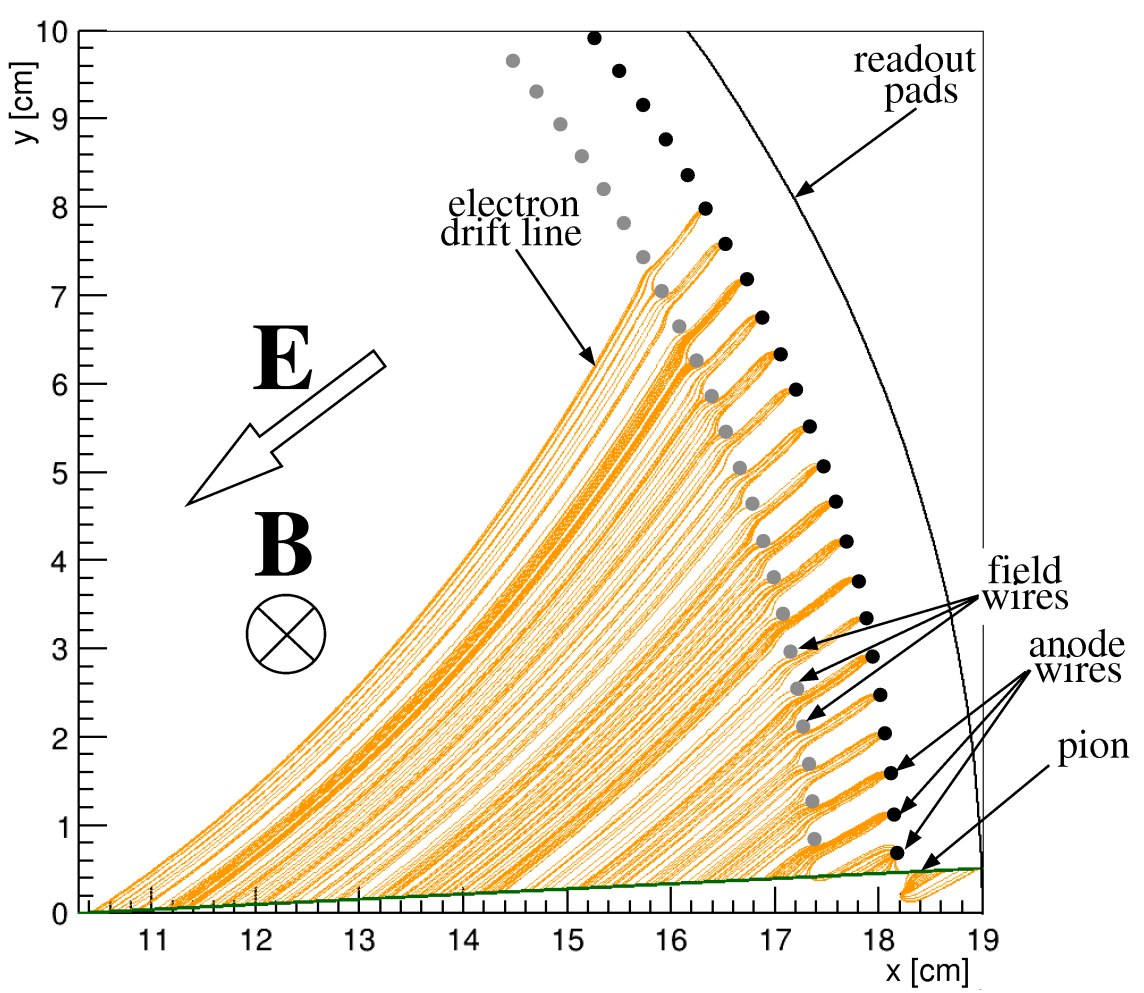
\includegraphics[width=\textwidth]{alpha-g_drift.png}
						\caption{Cross section view of the \ac{rTPC} (\garfieldpp simulation). The electrons (orange) produced by a~pion track (green) drift towards the anode wires, while influenced by the axial magnetic field. The size of the field and anode wires is exaggerated.}
						\label{fig:alpha-g_drift}
					\end{subfigure}
					\caption{Schematic view of the \acs{ALPHA}\protect\nobreakdash-g detector~\cite{alpha_rtpc}.}
				\end{figure}
				
				The $r$\nobreakdash-coordinate of the ionization cluster is reconstructed from the drift time using a~tabulated space-time relation. The 3D position of the interaction (cluster) vertex is obtained by matching the wires and pads by drift time using a~k\nobreakdash-d tree algorithm. Reconstructed tracks are fitted with a~helix via least squares~\cite{alpha_reco}.
	
	\section{Readout}
	\label{sec:readout}
		\subsection{Multi-Wire Proportional Chamber}
		\label{sec:MWPC}
			In most \acp{TPC} operated in experiments, a~\acf{MWPC} was used for the readout (\cref{fig:mwpc}). The electrons enter the chamber through a~cathode grid and are accelerated by a~strong electric field towards the parallel, thin anode wires creating an avalanche that multiplies the signal. The trajectory can be reconstructed from the drift time and two coordinates measured using
			\begin{enumerate}[nosep,label=\alph*)]
				\item two segmented cathodes (wires or strips) rotated by $\ang{90}$ or
				\item the ratio of charge collected on two ends of the resistive wires.
			\end{enumerate}
			For high counting rates, the positive ions from the avalanches accumulate, creating a~space charge that distorts the electric field. This can be mitigated by using a~gating grid near the readout plane to collect these ions at the cost of introducing a~dead time in the detector.
			
			\begin{figure}
				\centering
				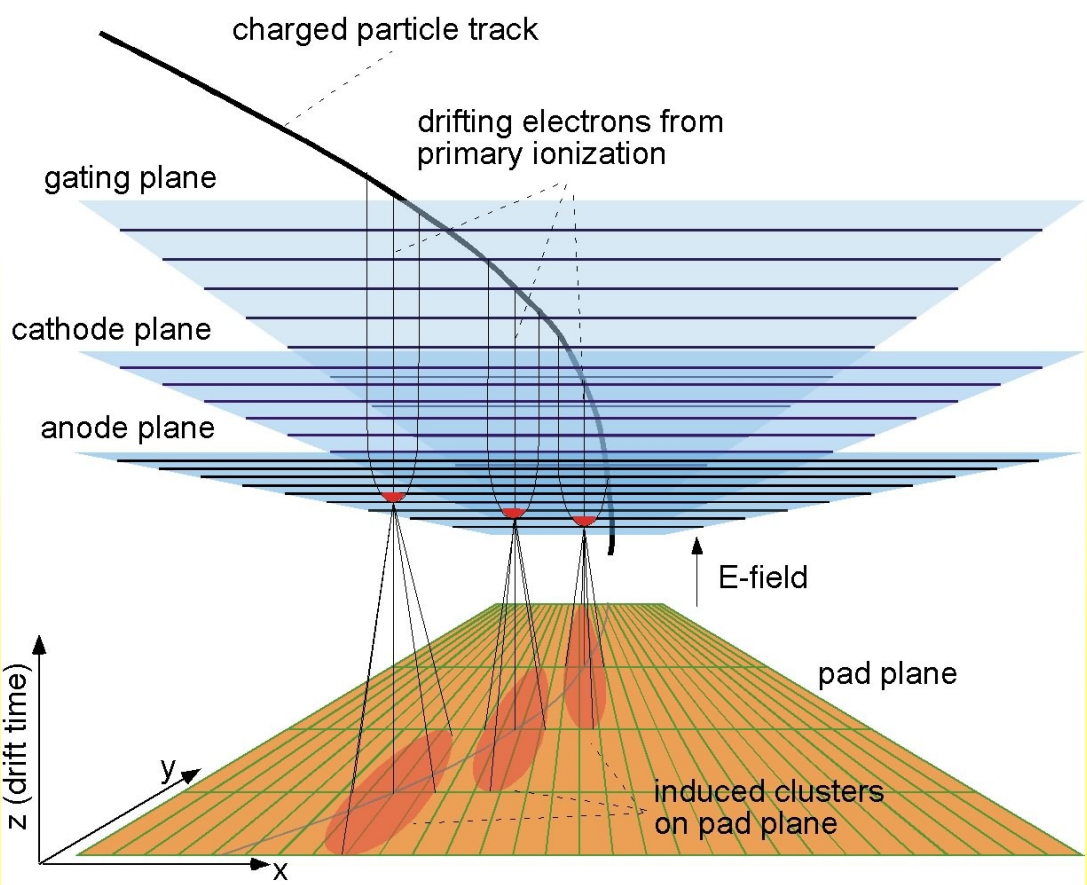
\includegraphics[width=0.7\textwidth]{mwpc.png}
				\caption{Schematic view of the ALICE \ac{MWPC} readout (working principle)~\cite{mwpc}.}
				\label{fig:mwpc}
			\end{figure}
			
		\subsection{Micro-Pattern Gaseous Detectors}
		\label{sec:mpgd}
			To overcome \ac{MWPC} limitations (e.g., diffusion, wire $\mathbf{E}\cross\mathbf{B}$ effect, space charge effects), a~family of \acf{MPGD} technologies are being developed. The readouts can reach higher spatial resolution (down to $\qty{30}{\um}$) with faster response time ($\unit{\ns}$ range) and much higher rate capability.
			
			\subsubsection{Gas Electron Multiplier}
				A~\acf{GEM} is a~thin metal-coated polyimide sheet with a~dense pattern of small, chemically etched holes (\cref{fig:gem}). The amplification is achieved by applying voltage difference across the metal layers and placing the foil between two moderate uniform electric fields. This creates a~strong electric field inside the holes that accelerates the incoming electrons and causes avalanches (see \cref{fig:gemsim}). Some charges may land on the dielectric surfaces due to diffusion, modifying the field and affecting gain.
				
				\begin{figure}
					\centering
					\begin{subfigure}[t]{0.48\textwidth}
						\centering
						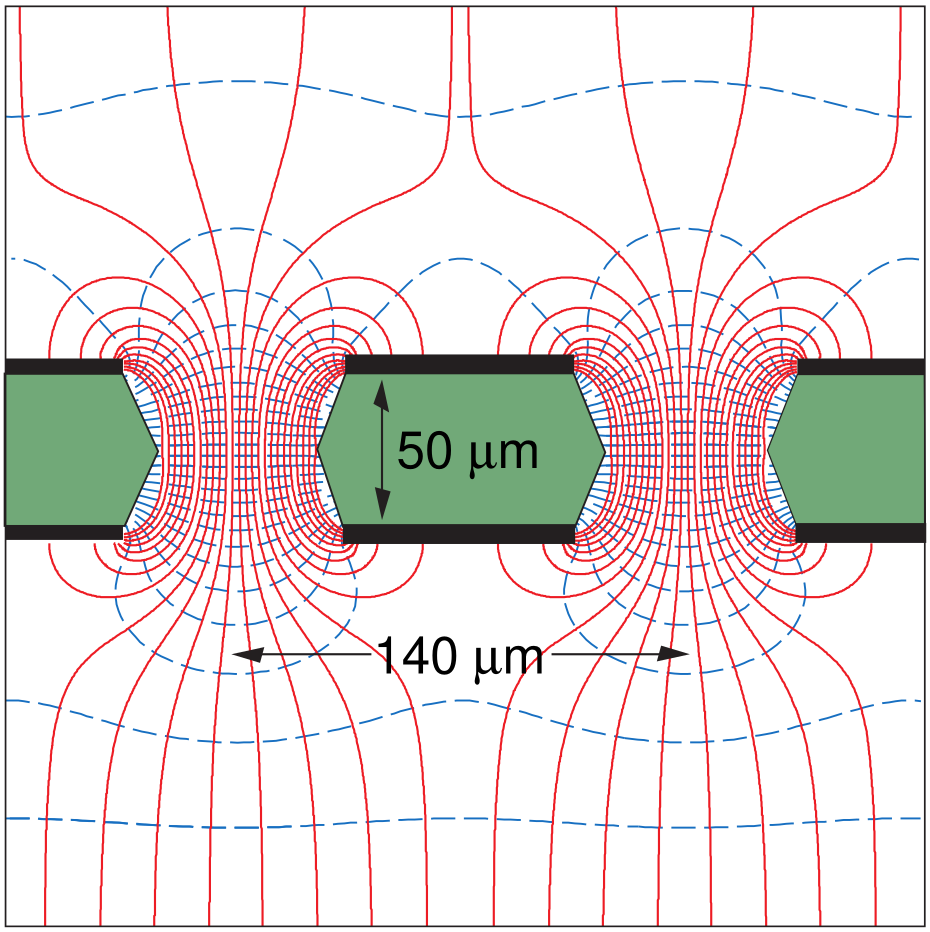
\includegraphics[width=\textwidth]{gem_schem.png}
						\caption{A~schematic view of a~\ac{GEM} cell with its typical dimensions, electric field lines (red), and equipotentials (blue)~\cite{pdg2024}.}
						\label{fig:gem_schem}
					\end{subfigure}
					\hfill
					\begin{subfigure}[t]{0.48\textwidth}
						\centering
						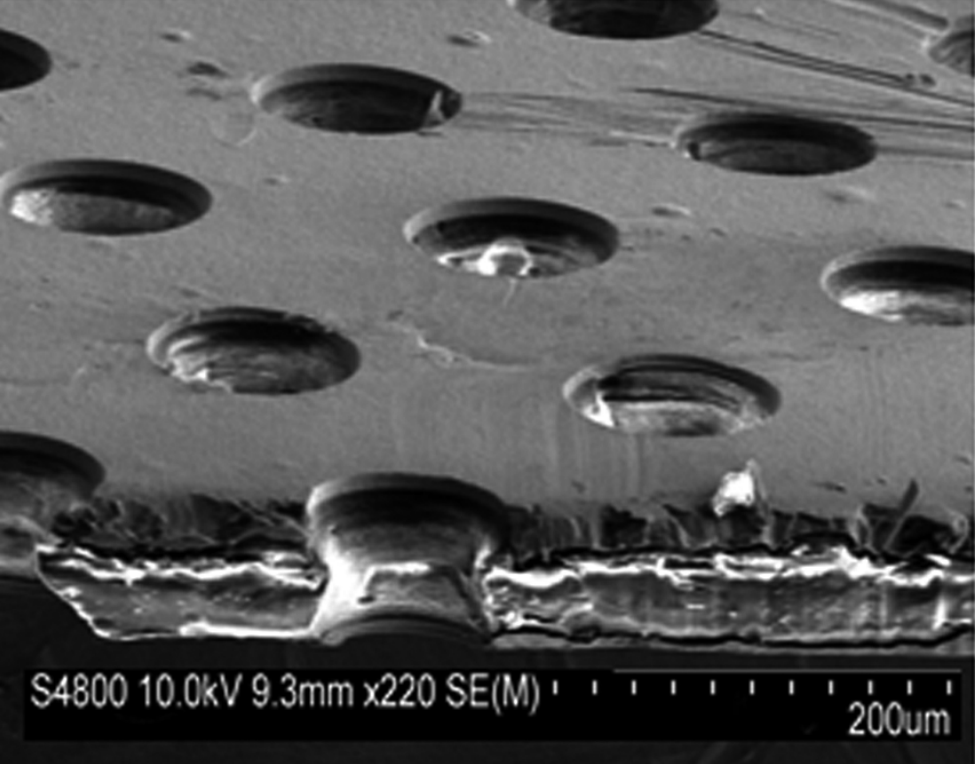
\includegraphics[width=\textwidth]{gem_hole.png}
						\caption{A~scanning electron microscope image of a~\ac{GEM} foil~\cite{gemhole}.}
						\label{fig:gemhole}
					\end{subfigure}
					\caption{\acf{GEM}.}
					\label{fig:gem}
				\end{figure}
				\begin{figure}
					\centering
					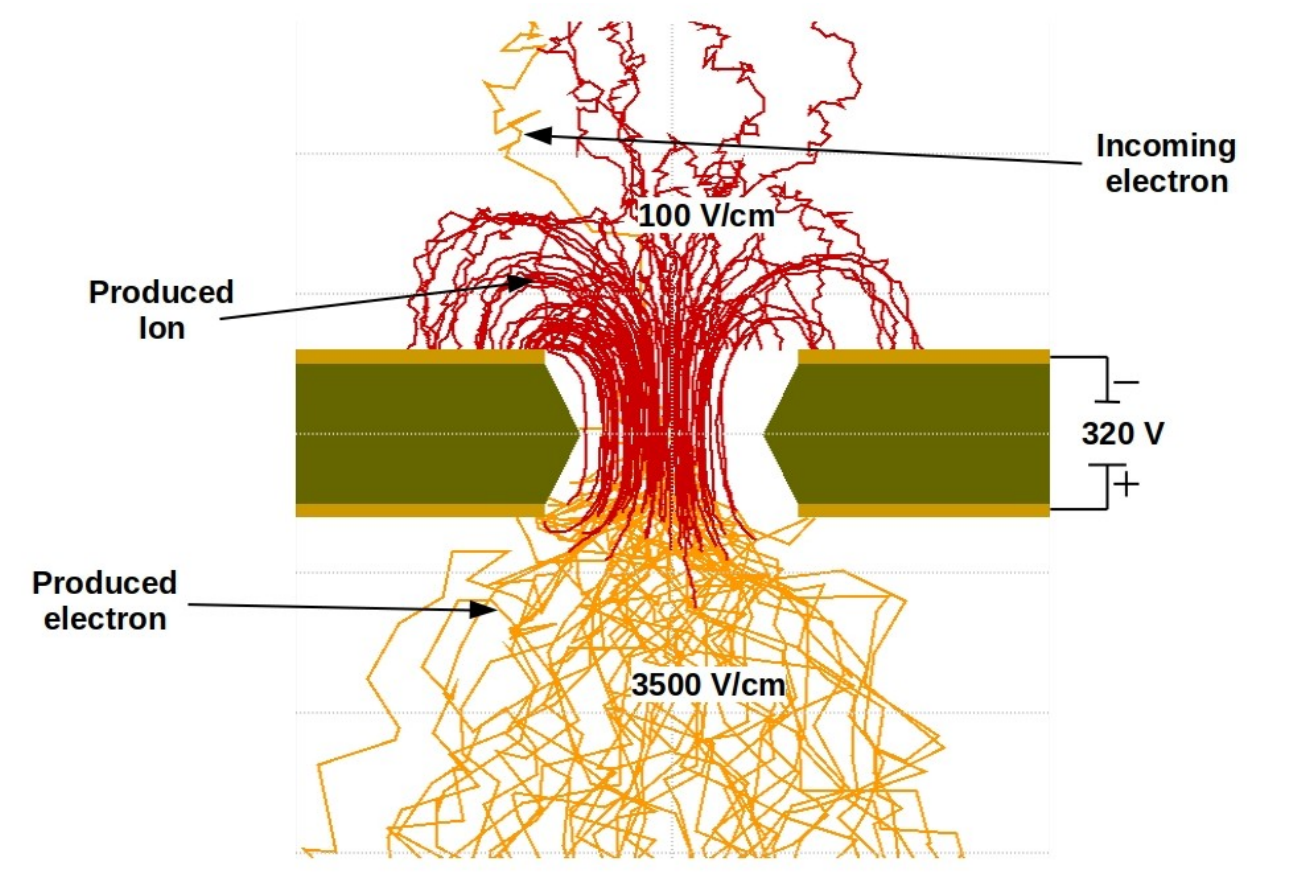
\includegraphics[width=0.8\textwidth]{gemsim.png}
					\caption{Garfield simulation of an avalanche in a~\ac{GEM} hole~\cite{gemsim}. An incoming electron (orange) is accelerated in the strong electric field of the \ac{GEM} and causes further ionization multiplying the number of free electrons (orange). Most of the produced cations (red) are captured by the \ac{GEM} cathode.}
					\label{fig:gemsim}
				\end{figure}
				
				Double or triple stacks of \acp{GEM} are usually used to create a~sufficient gain while maintaining stability (reducing discharges). From the last foil, the electrons drift to a~segmented anode where the signal is read. The ion backflow is reduced compared to \ac{MWPC}.
				
				A~cheaper alternative (especially for large area coverage) is a~\ac{THGEM} with a~\textapprox10\nobreakdash-fold upscaling of geometrical parameters. It can be made by mechanically drilling holes into a~standard \ac{PCB} and creating a~circular rim around the holes by etching the metal coating.
			
			\subsubsection{Micromegas}
				In a~\ac{Micromegas}, electrons pass through a~fine mesh (made out of very thin wires) into a~narrow amplification gap where they are multiplied in the high field and read as a~signal on the segmented anode (\cref{fig:micromegas_schem}). A~very high field (\qtyrange{30}{80}{\kV\per\cm}) is necessary to achieve sufficient gain. Ion backflow is heavily suppressed by the mesh. 
				
				A~Timepix chip (a~high granularity pixel detector) can be used for the readout anode to achieve the best spatial resolution, making an integrated readout called GridPix (\cref{fig:micromegas_sem}). Thanks to the high spatial resolution, it is possible to distinguish individual electron clusters, which enables a~new method of particle identification.
				
				\begin{figure}
					\centering
					\begin{subfigure}[t]{0.54\textwidth}
						\centering
						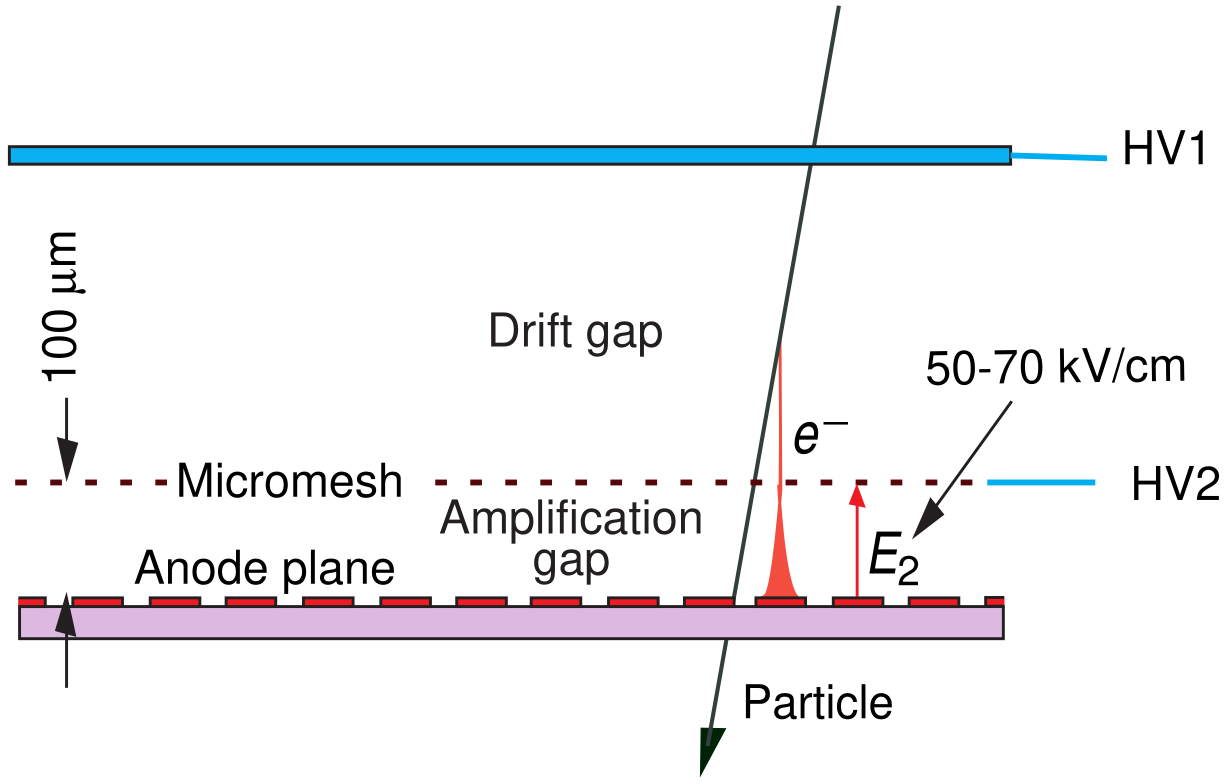
\includegraphics[width=\textwidth]{micromegas_schem.png}
						\caption{A~schematic view of a~\ac{Micromegas} detector.}
						\label{fig:micromegas_schem}
					\end{subfigure}
					\hfill
					\begin{subfigure}[t]{0.44\textwidth}
						\centering
						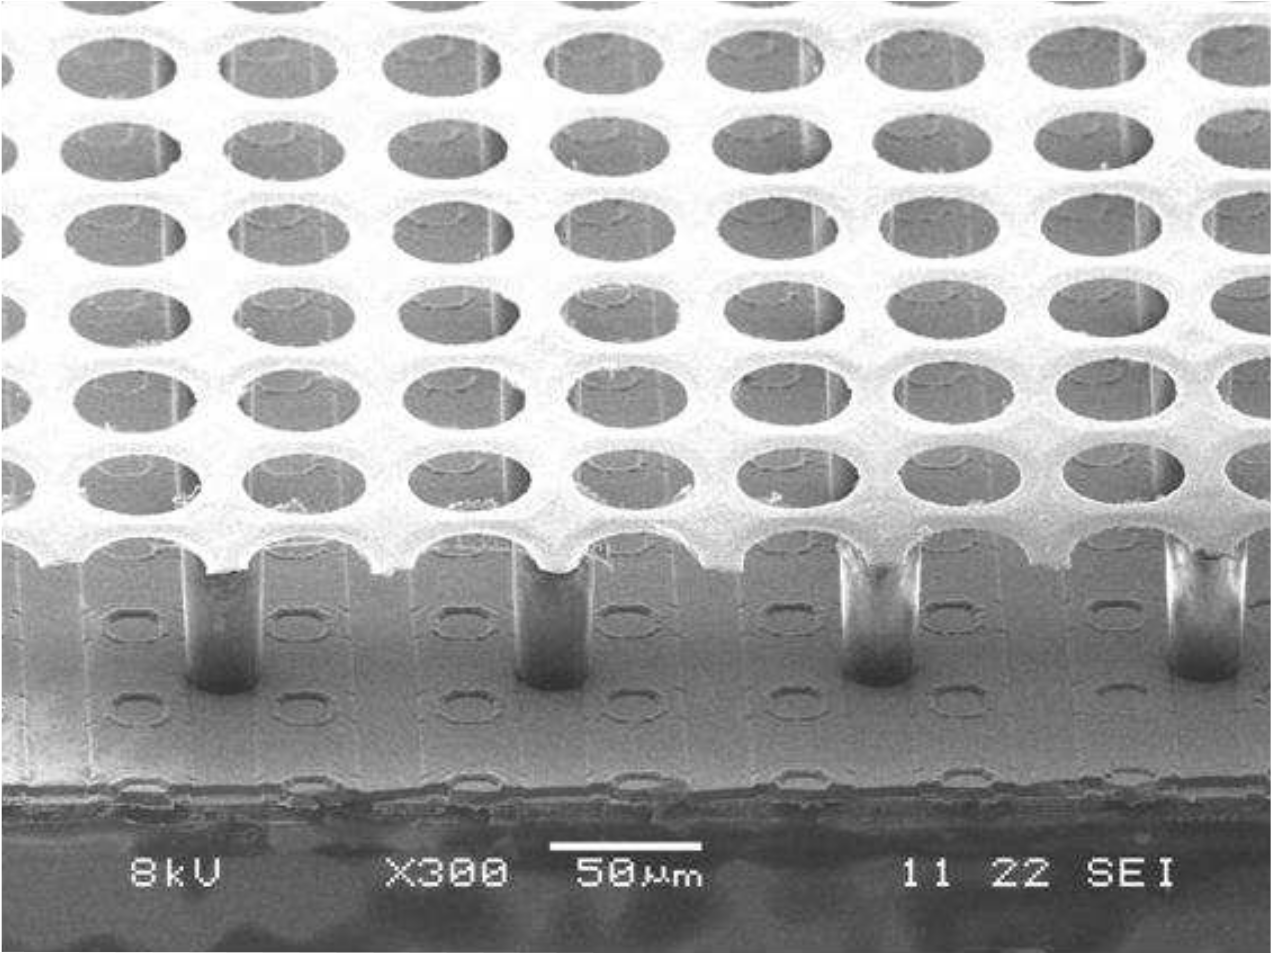
\includegraphics[width=\textwidth]{micromegas_sem.png}
						\caption{A~scanning electron microscope image of a~\ac{Micromegas} "GridPix" detector.}
						\label{fig:micromegas_sem}
					\end{subfigure}
					\caption{\acf{Micromegas}~\cite{pdg2024}.}
					\label{fig:micromegas}
				\end{figure}
			
			\subsubsection{Other MPGDs}
				A~\ac{RPWELL} consists of a~\ac{THGEM} with only the top side metal-coated, mounted on a~resistive film deposited on a~thin isolating sheet (which is read out similarly to a~\ac{RPC}). Due to the higher field in the closed holes of the \ac{THGEM}, a~higher gain can be reached for the same voltage. A~\ac{uRWELL} is a~similar architecture with \textapprox7~times smaller pitch (distance between holes). These options provide better spark resistance and could allow covering large areas for a~lower cost.
				
				A~\ac{uPIC} is a~\ac{PCB} with anode strips on one side and orthogonal cathode strips on the other. The cathode has a~resistive coating and a~regular pattern of uncoated regions with anode "dots" penetrating the \ac{PCB} at the centers.
	
	\section{Orthogonal Fields TPC at IEAP CTU}
	\label{sec:oftpc}
		At \ac{IEAPCTU}, we are going to use six identical atypical \acp{TPC} with an inhomogeneous toroidal magnetic field \textbf{orthogonal} to the electric field, hereafter referred to as \acf{OFTPC}. It has the shape of an isosceles trapezoidal prism with a~height of \qty{16}{\cm} with a~triple\nobreakdash-\ac{GEM} readout on one of its bases. Dimensions of the \ac{OFTPC} are discussed in detail in \cref{sec:coor} below. Throughout this thesis, we assume a~uniform electric field along the $z$~axis with $E_z = -\qty{400}{\V\per\cm}$. Measured particles enter the \ac{OFTPC} through a~window after crossing the \ac{MWPC}.
		
		
		\subsection{Motivation and Associated Challenges}
			The reasons for the unusual field layout are mostly related to construction feasibility:
				\begin{enumerate}[nosep,label=\alph*)]
					\item we use permanent magnets instead of a~solenoid, and parallel fields are difficult to accomplish this way,
					\item granularity of the \ac{TPC} readout is limited in order to fit one SAMPA/SRS hybrid in each sector -- parallel fields would bend the trajectories parallel to the readout requiring more pads and a~different architecture.
				\end{enumerate}
			In this thesis, we will show that such a~setup can reach a~similar energy resolution as common cylindrical \acp{TPC} while reducing the overall cost.
			
			The layout introduces two complications to the track reconstruction: the trajectory in the inhomogeneous field is not circular, and the drift is distorted by the magnetic field as shown in \cref{eq:drift} (in our case $\omega\tau \approx 0.08$\footnote{This is the approximate value in the strongest field based on charged mobility computed from the fitted drift velocity in \cref{sec:rasd}.}). We will deal with these effects in the upcoming chapters.
			
			The diffusion in such a~setup is larger since the parallel orientation reduces diffusion by curling the electrons in the $x$\nobreakdash-$y$ direction (see \cref{eq:difmag}), but for our relatively weak magnetic field and short drift distance, the difference is negligible.
	
		\subsection{Coordinate Systems and Dimensions}
		\label{sec:coor}
			In order to describe events in our detector, we use three distinct spaces: the detector space $\mathcal{D}$, the readout space $\mathcal{R}$, and the pad space $\mathcal{P}$. Each space is later used to represent ionization electrons at different stages of the detection process: their creation in the gas, their final position when hitting the readout plane, and finally their representation in the discrete pad space.
		
			\subsubsection{Detector Space}
				The detector space $\mathcal{D}$ represents the physical space of our detector. We describe it using Cartesian coordinates $(x,y,z)$. The $z$-axis is the detector's axis of symmetry, with its negative direction aligned with the proton beam. The origin $(0,0,0)$ is located at the center of the irradiated target. The positive $x$\nobreakdash-axis passes through the center of one of the \acp{OFTPC} along the intersection of its two planes of symmetry. The $y$\nobreakdash-axis is then chosen to maintain a~right-handed coordinate system.
				
				Since the detector has a~hexagonal symmetry, we use only one of its sectors in this work -- the first sector $\mathcal{D}_1 \subset \mathcal{D}$ which is defined by the condition:
					\begin{equation}
						(x,y,z) \in \mathcal{D}_1 \Leftrightarrow |y| \leq x\tan \frac{\pi}{6}.
					\end{equation}
				Simulations in this sector can be applied to all sectors by rotating the coordinates accordingly. The volume of the \ac{OFTPC} in this sector, which has the shape of a~trapezoidal prism, has these boundaries:
					\begin{align}
						x \in [x_\text{min},x_\text{max}] &= [\qty{6.51}{\cm},\qty{14.61}{\cm}],\\
						z \in [z_\text{min},z_\text{max}] &= [\qty{-8}{\cm},\qty{8}{\cm}],\\
						y_\text{max}(x_\text{min}) = -y_\text{min}(x_\text{min}) &= \qty{2.75}{\cm},\\
						y_\text{max}(x_\text{max}) = -y_\text{min}(x_\text{max}) &= \qty{7.45}{\cm},
					\end{align}
				where $y_\text{max}(x)$ is the maximal value of the $y$-coordinate for a~given $x$. The readout is located at $z = \qty{8}{\cm}$; for some purposes, we also define the distance to the readout $d_\text{r} = \qty{8}{\cm}-z$ as an alternative to the $z$-coordinate.The \ac{OFTPC} window has width \qty{3.8}{\cm} and height \qty{4.0}{\cm}.
				
				We also use spherical coordinates $(r,\theta,\varphi)$ with the elevation angle~$\theta$ measured relative to the $xy$ plane. Angles~$\theta$ and~$\varphi$ are useful when describing the direction of $e^+/e^-$~tracks. Their maximal values considered for the initial direction in simulations are $\theta_\text{max} \approx \qty{17.1}{\degree}$ and $\varphi_\text{max} \approx \qty{16.3}{\degree}$ as shown in \cref{fig:oftpc}.
				
				\begin{figure}
					\centering
					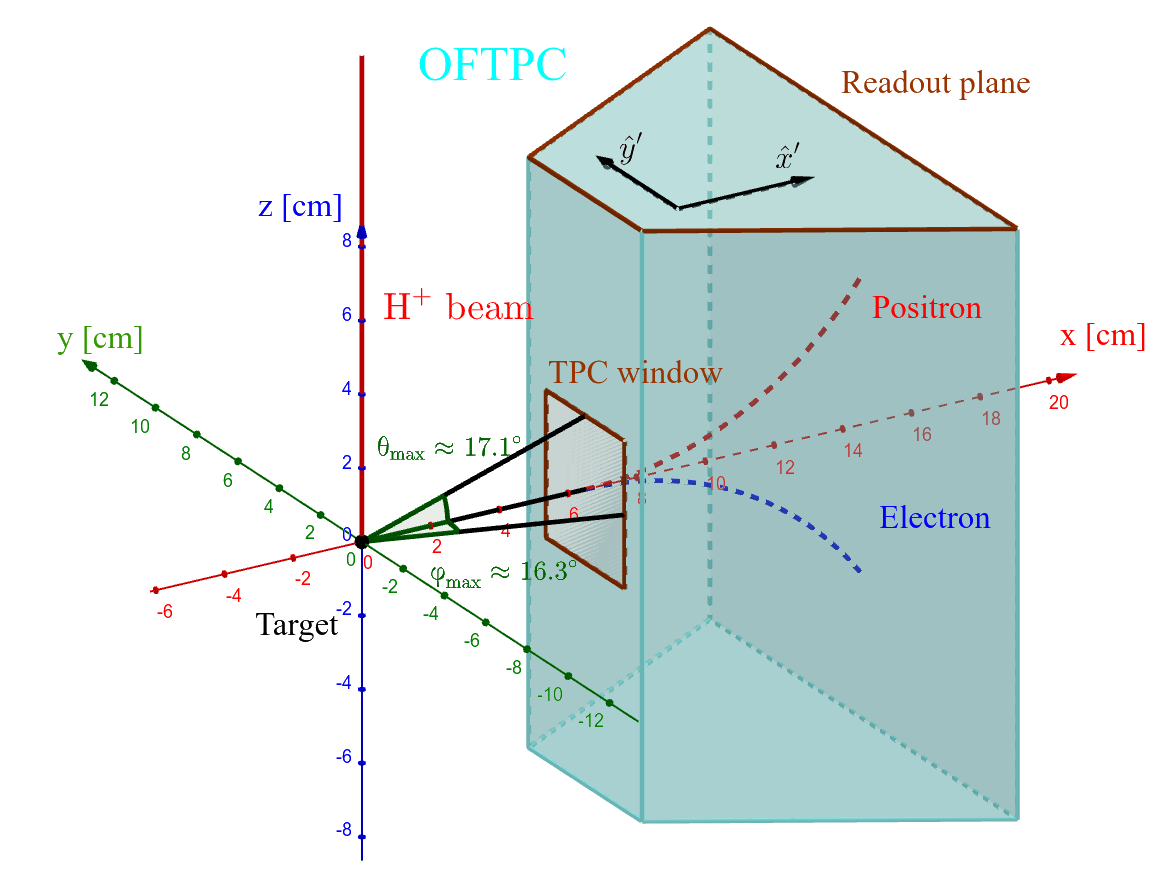
\includegraphics[width=0.8\textwidth]{tpc_ggb.png}
					\caption{Schematics of the first sector \ac{OFTPC} with detector space coordinates. Made with GeoGebra®.}
					\label{fig:oftpc}
				\end{figure}
			
			\subsubsection{Readout Space}
				The readout space $\mathcal{R}$ represents the drift time and final positions of ionization electrons as measured by an ideal continuous readout. We describe it using coordinates $(x',y',t)$, where $x'$ and $y'$ correspond to the detector coordinates at the readout plane ($z = 8$~cm). The drift time~$t$ is approximately proportional to the distance to the readout $d_r$.
			
			\subsubsection{Pad Space}
				The pad space $\mathcal{P}$ represents the time bin and pad number of ionization electrons as measured by an ideal discrete readout:
					\begin{equation}
						\mathcal{P} = \{(n_\text{pad},n_t)\in\mathbb{N}^2 \mid n_\text{pad}\leq128\}.
					\end{equation}
				It is a~discretization of a~certain volume in $\mathcal{R}$ that can be obtained from simulations.
				
				The readout of the \ac{OFTPC} will consist\red{~(is the design final?)} of 128~rectangular pads arranged in a~staggered pattern. Parameters of the pad layout are shown in \cref{fig:padlayout}. The bottom left corner of $n$\nobreakdash-th pad has coordinates $(x_{1,n},y_{1,n})$, the top right $(x_{2,n},y_{2,n})$ and its center has coordinates $(x_{c,n},y_{c,n})$. The gap between neighboring pads is $g=\qty{0.08}{\cm}$; we consider it being shared equally between the neighboring pads. Time will be read out in discrete bins of size $t_\text{bin}=\qty{100}{\ns}$.
			
				\begin{figure}[H]
					\centering
					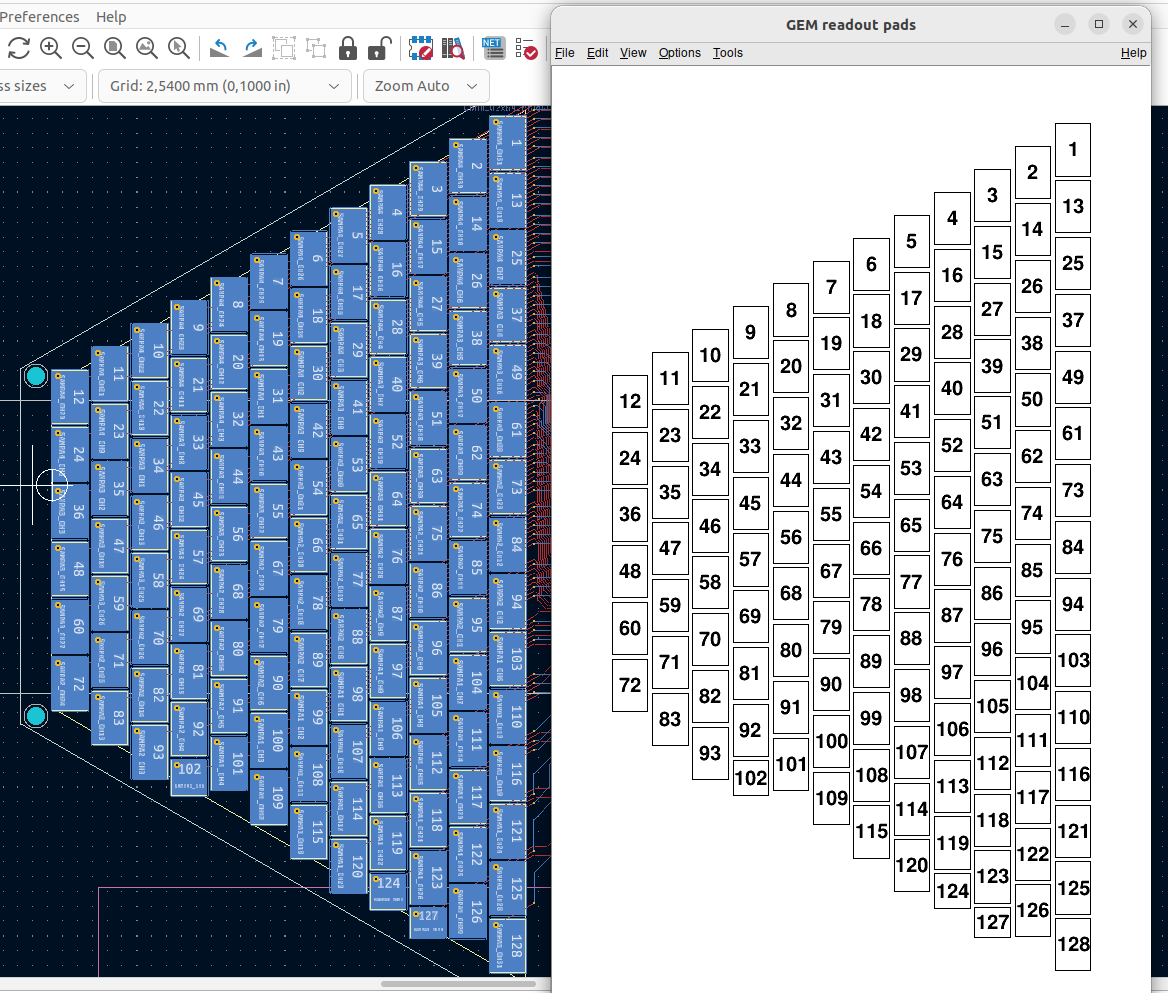
\includegraphics[width=\textwidth]{padlayout.png}
					\caption{Pad layout of the \ac{OFTPC} and its parameters. Pads 102, 124, and 127 are irregular, the rest have the same dimensions.}
					\label{fig:padlayout}
				\end{figure}
		
		\subsection{Magnetic Field Simulation}
		\label{sec:mag}
			The magnetic field inside our detector is produced by six permanent magnets. It was simulated using Ansys Maxwell~\cite{ansys_maxwell}, which gives us values on a~regular grid. Visualization of the magnetic field is shown in \cref{fig:mag}. Whenever we need to work with values outside this grid, we use trilinear interpolation described below.
			
			\begin{figure}
				\centering
				\begin{subfigure}[t]{0.45\textwidth}
					\centering
					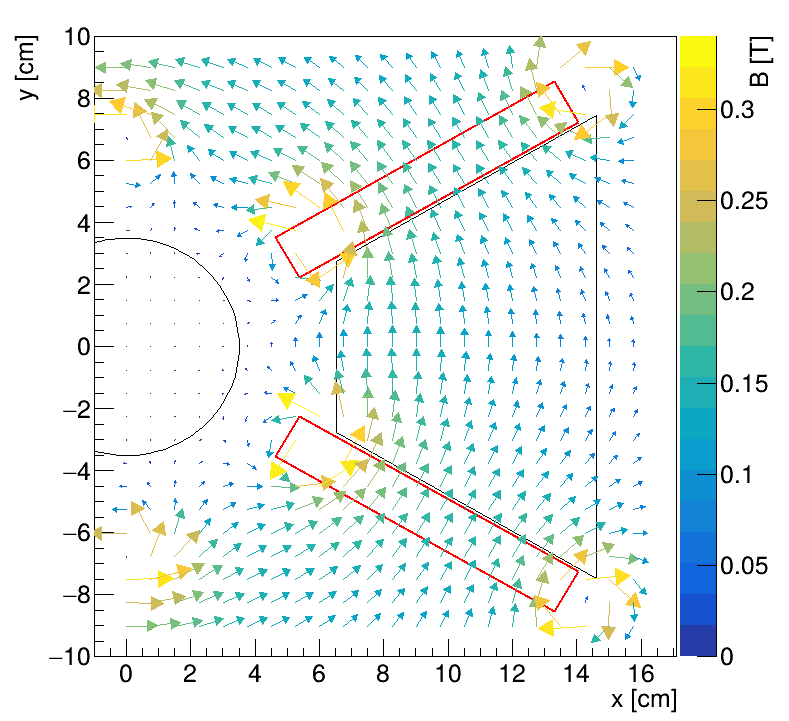
\includegraphics[width=\textwidth]{mag_xy.png}
					\caption{Field in the $xy$ plane.}
				\end{subfigure}
				\hfill
				\begin{subfigure}[t]{0.45\textwidth}
					\centering
					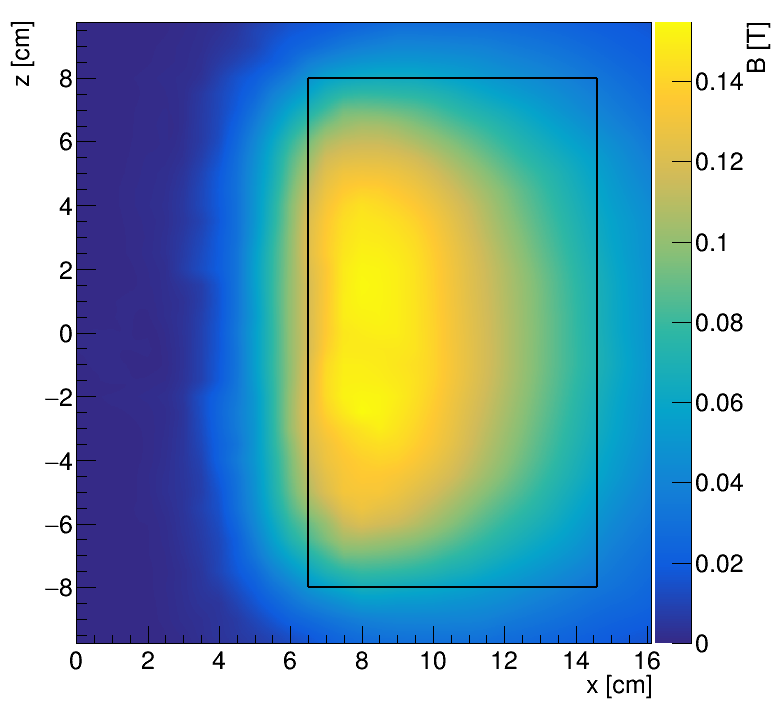
\includegraphics[width=\textwidth]{mag_xz.png}
					\caption{Field magnitude in the $xz$ plane.}
					\label{fig:mag_xz}
				\end{subfigure}
				\caption{Magnetic field simulation results. The \ac{OFTPC} volume and the vacuum tube are marked with black lines; the magnets are marked with red lines. In the current design of the real detector, magnets are slightly shifted compared to the simulation.}
				\label{fig:mag}
			\end{figure}
		
			\subsubsection{Trilinear Interpolation}
			\label{sec:trilin}
				Trilinear interpolation is a~3D generalization of linear interpolation\footnote{Linear interpolation in point $x\in(x_1,x_2)$ of a~function $f\colon\mathbb{R}\to\mathbb{R}$ known in points $x_1 < x_2$ is the convex combination $\widehat{f}(x) = (1-x_d)f(x_1)+x_d f(x_2)$, where $x_d = \frac{x-x_1}{x_2-x_1} \in (0,1)$.}. It can be used to interpolate a~function whose values are known on a~regular grid with rectangular prism cells. We use this simple method for interpolating the magnetic field, and it is later used in \cref{sec:grad} to interpolate the Ionization Electron Map, a~key component of our track reconstruction algorithm. In both cases, we use a~regular cubic grid (also known as a~Cartesian grid).
				
				Let us consider a~cell of our regular grid (a~cube) with an edge length~$a$ containing the point $\mathbf{C} = (x,y,z)$ where we want to interpolate a~function $f\colon\mathbb{R}^3\to\mathbb{R}$. We know the values of this function at the vertices of the cell $\mathbf{C}_{ijk} = (x_0+ia,y_0+ja,z_0+ka)$, where $\mathbf{C}_{000} = (x_0,y_0,z_0)$ is the origin of the cell, and $i,j,k \in \{0,1\}$ are indices. We also define the points $\mathbf{C}_{ij} = (x,y_0+ia,z_0+ja)$ and $\mathbf{C}_i=(x,y,z_0+ia)$. Then the interpolated value $\widehat{f}(\mathbf{C})$ can be calculated as a~composition of three linear interpolations (see \cref{fig:trilin}):
					\begin{alignat}{3}
						\label{eq:linterpol}
						\widehat{f}(\mathbf{C}_{ij}) &= (1-x_d)\,f(\mathbf{C}_{0ij}) \,&+&\,x_d\, f(\mathbf{C}_{1ij}),\\
						\label{eq:linterpol2}
						\widehat{f}(\mathbf{C}_{i}) &= (1-y_d)\,\widehat{f}(\mathbf{C}_{0i}) &+&\,y_d\, \widehat{f}(\mathbf{C}_{1i}),\\
						\label{eq:linterpol3}
						\widehat{f}(\mathbf{C}) &= (1-z_d)\,\widehat{f}(\mathbf{C}_0) &+&\,z_d\, \widehat{f}(\mathbf{C}_1),
					\end{alignat}
				where $x_d$, $y_d$, and $z_d$ are given as follows:
					\begin{equation}
						x_d = \frac{x-x_0}{a},~y_d = \frac{y-y_0}{a},~z_d = \frac{z-z_0}{a}.
					\end{equation}
					
				\begin{figure}
					\centering
					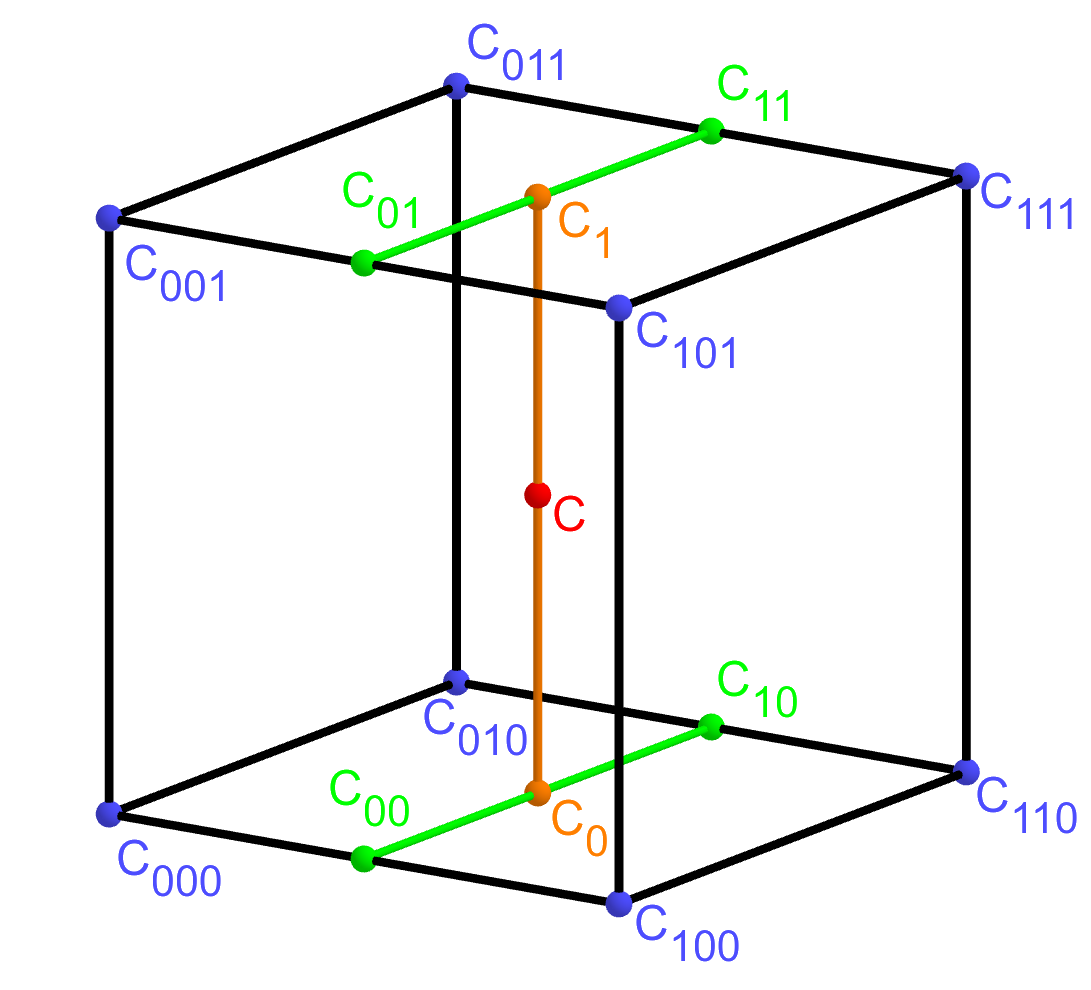
\includegraphics[width=0.5\textwidth]{trilinear.png}
					\caption{Visualization of trilinear interpolation as a~composition of linear interpolations (inspired by~\cite{trilinear1}). We want to interpolate the value in the red point~$\mathbf{C}$. First, we interpolate between the four pairs of blue points sharing the last two indices along the $x$\protect\nobreakdash-axis (\cref{eq:linterpol}), then between the two pairs of the resulting green points along the $y$\protect\nobreakdash-axis (\cref{eq:linterpol2}), and finally between the two resulting orange points along the $z$\protect\nobreakdash-axis to get the final red value (\cref{eq:linterpol3}). Made with GeoGebra®.}
					\label{fig:trilin}
				\end{figure}
					
				\noindent We can also write
					\begin{equation}
						\label{eq:trilingeo}
						\widehat{f}(\mathbf{C}) = \sum_{i,j,k \in \{0,1\}} t_x^i t_y^j t_z^k f(\mathbf{C}_{ijk}),
					\end{equation}
				using a~vector
					\begin{equation}
						t_\alpha \stackrel{\text{def}}{=} \begin{pmatrix}t_\alpha^0\\ t_\alpha^1\end{pmatrix} = \begin{pmatrix}1-\alpha_d\\ \alpha_d\end{pmatrix},
					\end{equation}
				where $\alpha \in \{x,y,z\}$ is an index. This gives a~nice geometric interpretation to the trilinear interpolation as shown in \cref{fig:trilin2}. From this form and the figure, it is apparent that the final interpolated value does not depend on the order of axes along which we perform linear interpolations (see \cref{fig:trilin}). Furthermore, we can write $\widehat{f}(\mathbf{C})$ as a~polynomial:
					\begin{equation}
						\label{eq:trilinpoly}
						\widehat{f}(\mathbf{C}) = \sum_{\alpha,\beta,\gamma \in \{0,1\}}\sum^{\alpha}_{i=0}\sum^{\beta}_{j=0}\sum^{\gamma}_{k=0} 	(-1)^{(\alpha-i)+(\beta-j)+(\gamma-k)} f(\mathbf{C}_{ijk}) x_d^\alpha y_d^\beta z_d^\gamma.
					\end{equation}
				We take advantage of this form when generalizing trilinear interpolation to an irregular grid in \cref{sec:interpol}.
					%\begin{equation}
					%	\widehat{f}(C) = (1-x_d) (1-y_d) (1-z_d) f(C_{000}) + (1-x_d) (1-y_d) z_d f(C_{001}) + (1-x_d) y_d (1-z_d) f(C_{010}) + (1-x_d) y_d z_d f(C_{011}) + x_d (1-y_d) (1-z_d) f(C_{100}) + x_d (1-y_d) z_d f(C_{101}) + x_d y_d (1-z_d) f(C_{110}) + x_d y_d z_d f(C_{111})
					%\end{equation}
					
				\begin{figure}
					\centering
					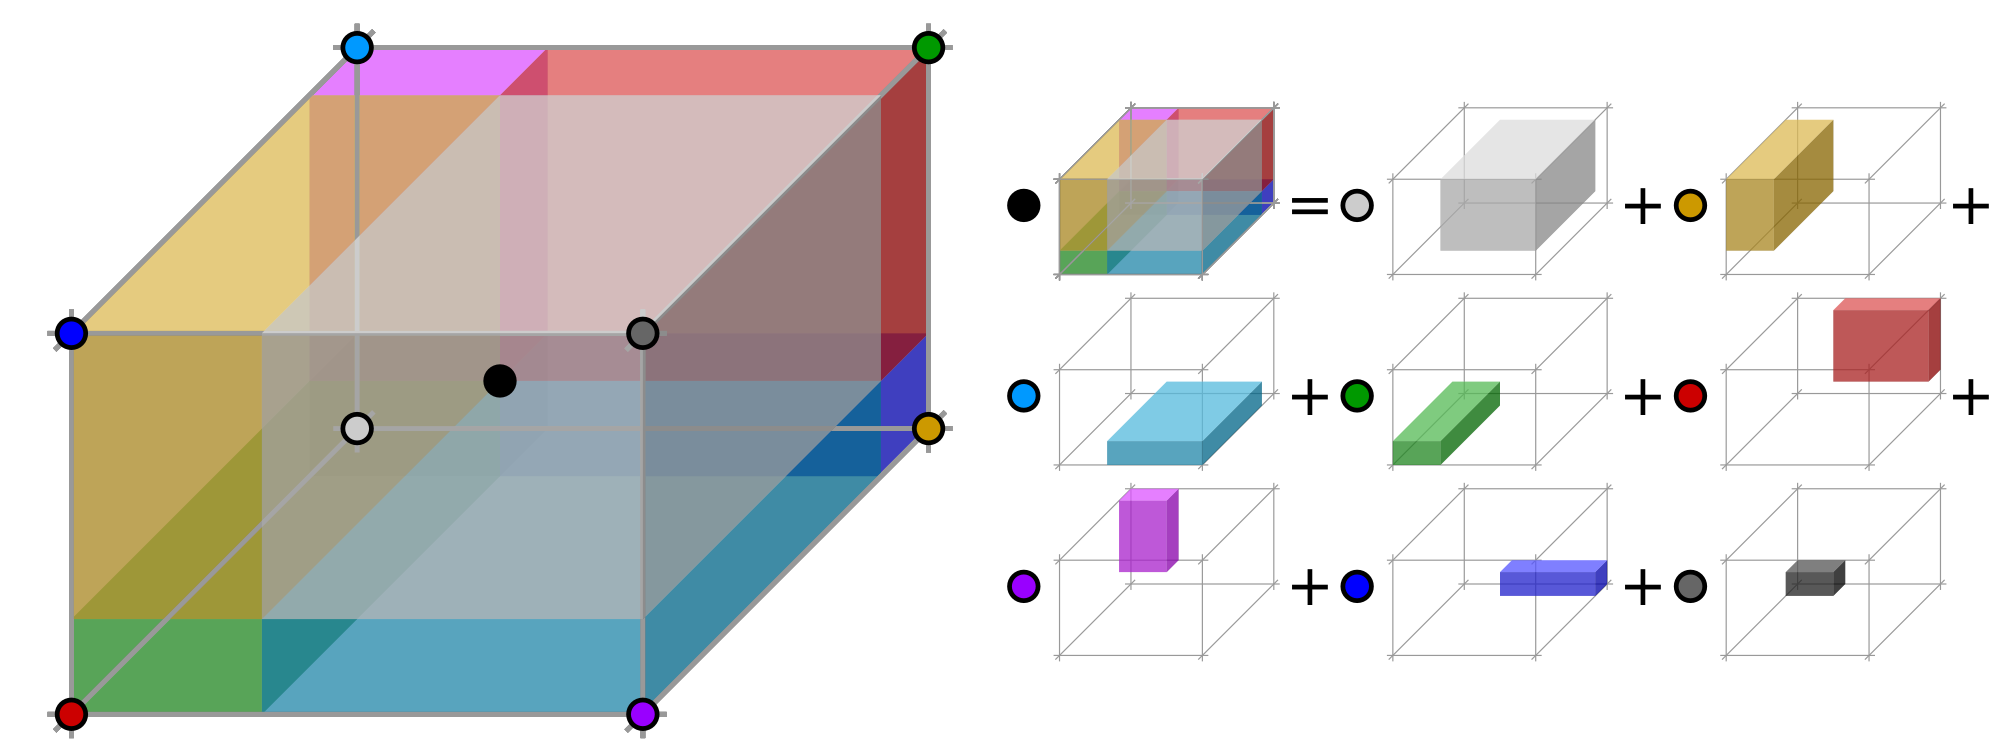
\includegraphics[width=\textwidth]{trilinear2.png}
					\caption{Geometric interpretation of trilinear interpolation as expressed in \cref{eq:trilingeo}. The colored dots represent the values in given points and the colored boxes represent the volume in the opposite corner by which the corresponding values are multiplied. The black dot represents the interpolated value which is multiplied by the entire volume~\cite{trilinear}.}
					\label{fig:trilin2}
				\end{figure}
	\chapter{Track Simulation}
	In order to develop and test the reconstruction algorithm, electron and positron tracks are simulated inside the first detector sector $\mathcal{D}_1$ (see Section~\ref{sec:coor}) with different initial parameters (origin, initial direction and kinetic energy). Two approaches are currently used to simulate tracks, each of them for different purpose.
	
	The \textbf{Microscopic Simulation} uses the \garfieldpp toolkit~\cite{Garfield++}. Within this toolkit:
		\begin{enumerate}[nosep,label=\alph*)]
			\item MagBoltz~\cite{magboltz} is used to calculate the transport properties,
			\item the \ac{HEED} program~\cite{HEED} is used to simulate the primary particle,
			\item the class \textit{AvalancheMicroscopic} to simulate the drift of secondary electrons created by ionization in the gas.
		\end{enumerate}
	This is the most precise and time-consuming simulation used; our current goal is to be able to successfully reconstruct its results and determine our best-case energy resolution.
	
	The \textbf{Runge-Kutta Simulation} uses the 4th order Runge-Kutta numerical integration to simulate the trajectory of the primary particle in the electromagnetic field inside the detector. It is relatively fast since it does not simulate the secondary particles. It is used as part of our reconstruction algorithm and for testing some parts of the reconstruction.
	
	All of these simulations require the knowledge of the electromagnetic field (both $\mathbf{E}$~and~$\mathbf{B}$) inside the detector. A~uniform electric field of 400~V$\cdot$cm$^{-1}$ is assumed. The magnetic field was simulated in Maxwell (see Section~\ref{sec:mag}).
	
	\section{Microscopic Simulation}
	\label{sec:microsim}
		The microscopic simulation, the most detailed simulation used in this work, is performed using the \garfieldpp toolkit~\cite{Garfield++}.
		
		The electron transport properties are simulated using the program Magboltz. Two different gas mixtures were compared -- 90:10 and 70:30 Ar:CO$_2$. The second mixture will be used in our detector. The temperature is set to 20~$^\circ$C, the pressure is atmospheric.
		
		The primary track is simulated using the program~\ac{HEED}, which is an implementation of the photo-absorption ionization model~\cite{HEED}. This program provides the parameters of ionizing collisions. \ac{HEED} can also be used to simulate the transport of delta electrons; we do not account for them in the current simulation. The photons created in the atomic relaxation cascade\blue{~(fluorescence reabsorption, related to the spread of avalanches in GM det.?)} are also not simulated.
		
		Finally, we use the microscopic tracking provided by the class \textit{AvalancheMicroscopic} in \garfieldpp to simulate the drift of the ionization electrons. Each electron is followed from collision to collision using the equation of motion and the collision rates calculated by Magboltz\red{~(how fast is this? maybe it slows down the simulation when spreading it across multiple jobs? --- remarks)}.
		
		\garfieldpp also contains two other classes for simulation of the drift. \texttt{AvalancheMC} uses Monte Carlo integration that requires generation of a gas file to approximate the transport parameters (we briefly considered this method, but decided that the relatively small speed wasn't worth the loss of precision in this case, especially since the gas file generation for different angles between the field vectors is also computationally expensive). \texttt{DriftlineRKF} uses Runge-Kutta-Fehlberg integration of a~phenomenological relation $\mathbf{v}_\text{d} = \mathbf{v}_\text{d}(\mathbf{E},\mathbf{B})$, and therefore cannot account for diffusion.
		
		\subsection{First testing track}
		\label{sec:microfirst}
			The first electron track simulated for testing purposes was chosen to have a~special set of parameters:
				\begin{itemize}[nosep]
					\item the starting point of the track is the origin of the coordinate system,
					\item the initial direction is along the positive $x$-axis,
					\item the momentum is $8~\text{MeV}/c$ (the kinetic energy is 7.505~MeV).
				\end{itemize}
			Such a~track moves in the XZ plane in the toroidal magnetic field of the detector, because the particle's velocity vector is always perpendicular to the field. At first, we simulated such a~track in 90:10 Ar:CO$_2$ gas mixture, later we added a~simulation in 70:30 Ar:CO$_2$, which we plan to use in our detector. The comparison of both simulations is in \cref{fig:microfirst}. In the first tests, the initial energy of produced ionization was set to \qty{0.1}{\eV} instead of the value generated by \ac{HEED}.
			
			\begin{figure}
				\centering
				\begin{subfigure}[t]{0.48\textwidth}
					\centering
					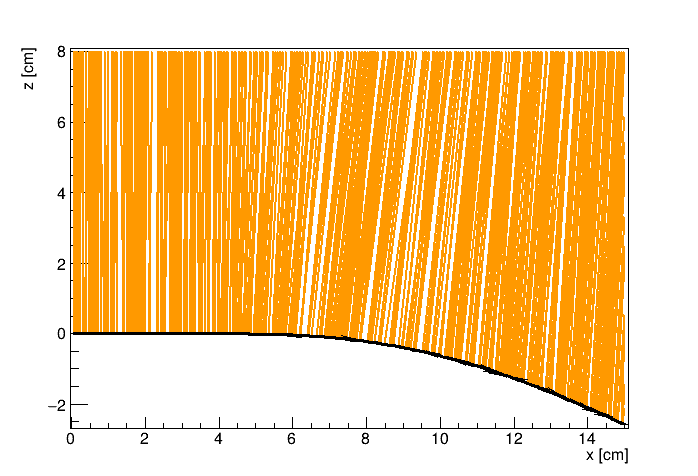
\includegraphics[width=\textwidth]{9010_xz.png}
					\caption{90:10 Ar:CO$_2$ drift lines XZ projection}
				\end{subfigure}
				\hfill
				\begin{subfigure}[t]{0.48\textwidth}
					\centering
					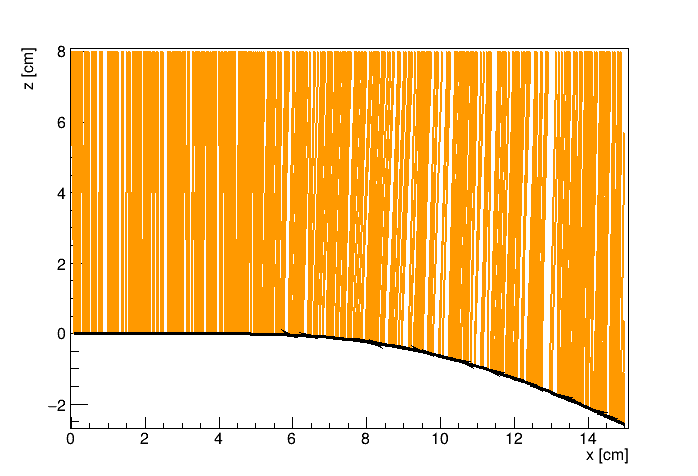
\includegraphics[width=\textwidth]{7030_xz.png}
					\caption{70:30 Ar:CO$_2$ drift lines XZ projection}
				\end{subfigure}
				\hfill
				\begin{subfigure}[t]{0.48\textwidth}
					\centering
					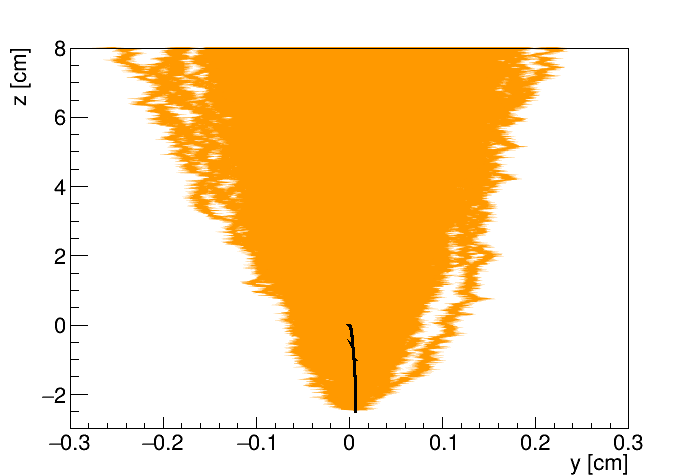
\includegraphics[width=\textwidth]{9010_yz.png}
					\caption{90:10 Ar:CO$_2$ drift lines YZ projection}
				\end{subfigure}
				\hfill
				\begin{subfigure}[t]{0.48\textwidth}
					\centering
					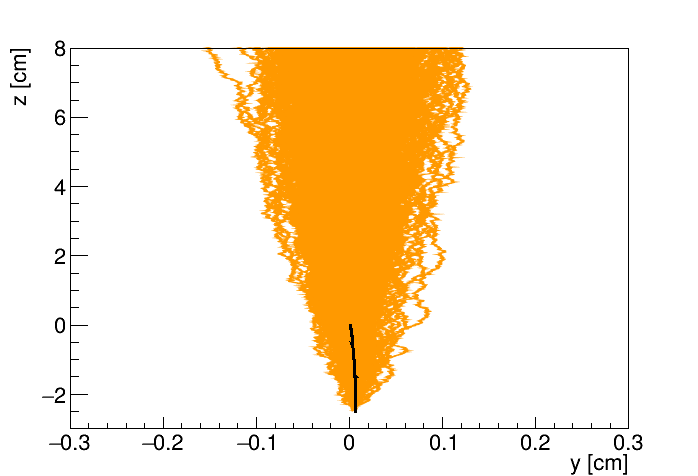
\includegraphics[width=\textwidth]{7030_yz.png}
					\caption{70:30 Ar:CO$_2$ drift lines YZ projection}
				\end{subfigure}
				\hfill
				\begin{subfigure}[t]{0.48\textwidth}
					\centering
					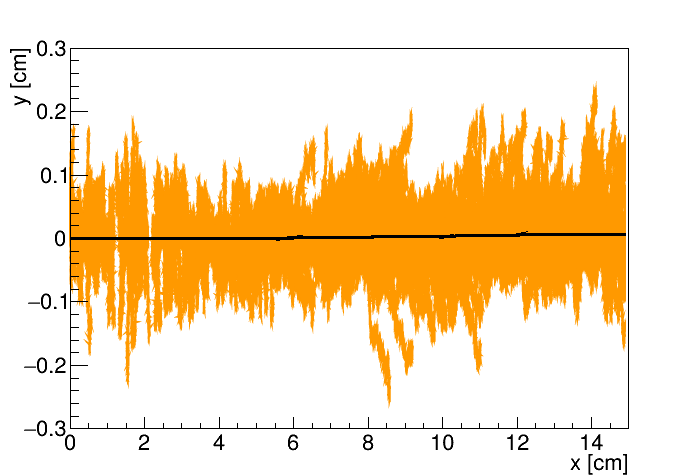
\includegraphics[width=\textwidth]{9010_xy.png}
					\caption{90:10 Ar:CO$_2$ drift lines XY projection}
				\end{subfigure}
				\hfill
				\begin{subfigure}[t]{0.48\textwidth}
					\centering
					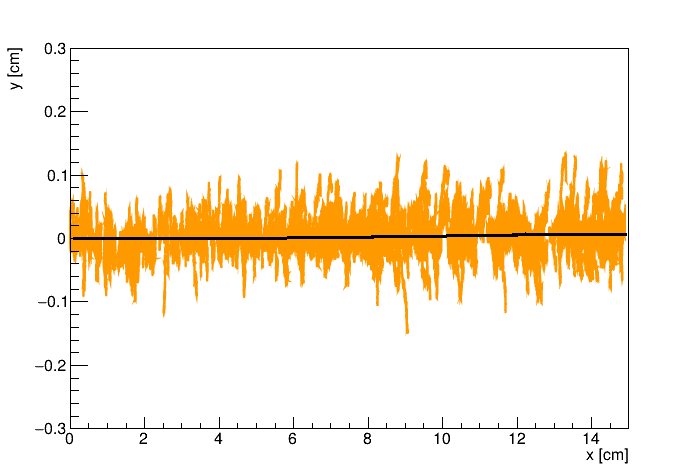
\includegraphics[width=\textwidth]{7030_xy.png}
					\caption{70:30 Ar:CO$_2$ drift lines XY projection}
				\end{subfigure}
				\caption{Comparison of drift lines for two different gas mixtures 90:10 and 70:30 Ar:CO$_2$. The electron track is marked in black, the drift lines of the ionization electrons are marked in orange. In this example, we assume a~larger \ac{OFTPC} volume with readout at $z = 8$~cm. Small curvature of the track in the YZ projection is caused by the tilt of the magnetic field in the bottom half of the \acf{OFTPC}.}
				\label{fig:microfirst}
			\end{figure}
			
		\subsection{Grid-like testing sample}
		\label{sec:microgrid}
			In order to test all steps of the reconstruction, a~sample of tracks with a~grid-like distribution of parameters was generated on MetaCentrum. Five sets of 9702 tracks were generated with every combination of these parameters:
				\begin{itemize}[nosep]
					\item electron and positron tracks,
					\item 11 different kinetic energies $E_\text{kin}\in[3,13]$~MeV,
					\item 21 different azimuth angles $\varphi \in [-16.3^\circ,16.3^\circ]$ and
					\item 21 different elevation angles $\theta \in [-17.1^\circ,17.1^\circ]$.
				\end{itemize}
			A~visualization of a~set of $e^+/e^-$~tracks with the same kinetic energy is shown in \cref{fig:microgrid}. In the 70:30 Ar:CO$_2$ atmosphere, each track takes 5-30~CPU hours to simulate. Every tenth point on the drift line was stored, the whole sample has 3.1~terabytes (or 1.4~gigabytes without drift lines).
			
				\begin{figure}
					\centering
					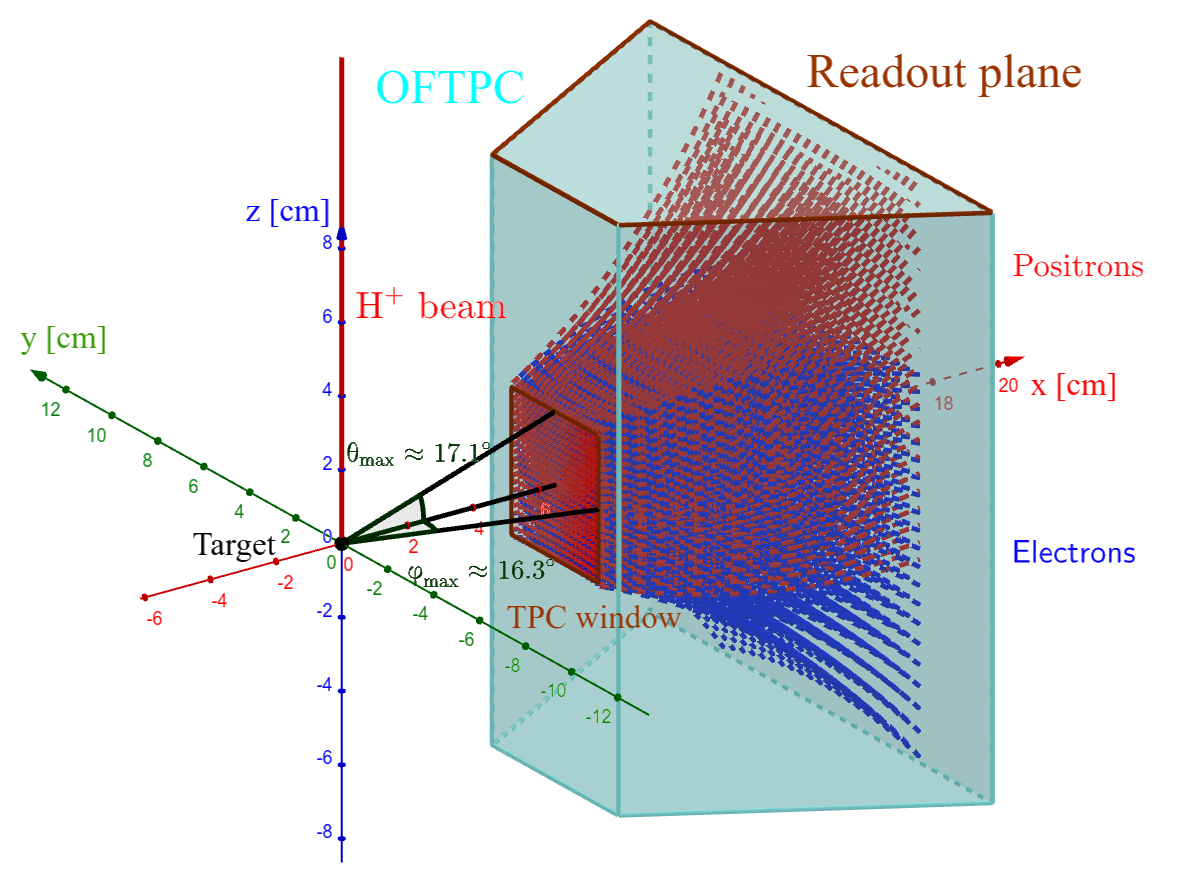
\includegraphics[width = 0.9\textwidth]{tpc_grid.png}
					\caption{A~visualization of a~set of tracks from the grid-like testing sample with the same kinetic energy.}
					\label{fig:microgrid}
				\end{figure}
	
	\section{Runge-Kutta Simulation}
	\label{sec:rks}
		The Runge-Kutta simulation in this work uses the \ac{RK4} method to numerically integrate the equation of motion of a~relativistic charged particle in an electromagnetic field. Given a~system of first order differential equations
			\begin{equation}
				\derivative{\mathbf{y}}{t}(t) = \mathbf{f}(t,\mathbf{y}(t))
			\end{equation}
		with an initial condition
			\begin{equation}
				\mathbf{y}(t_0) = \mathbf{y}_0,
			\end{equation}
		we iteratively compute the estimate $\mathbf{y}_n = \mathbf{y}(t_n) = \mathbf{y}(t_0+nh)$ as follows:
			\begin{align}
				\mathbf{k}_1 &= \mathbf{f}(t_n,\mathbf{y}_n),\\
				\mathbf{k}_2 &= \mathbf{f}\left(t_n+\frac{h}{2},\, \mathbf{y}_n+\frac{h\mathbf{k}_1}{2}\right),\\
				\mathbf{k}_3 &= \mathbf{f}\left(t_n+\frac{h}{2},\, \mathbf{y}_n+\frac{h\mathbf{k}_2}{2}\right),\\
				\mathbf{k}_4 &= \mathbf{f}(t_n+h,\, \mathbf{y}_n+h\mathbf{k}_3),
			\end{align}
			\begin{equation}
				\mathbf{y}_{n+1} = \mathbf{y}_n + \frac{1}{6}(\mathbf{k}_1+2\mathbf{k}_2+2\mathbf{k}_3+\mathbf{k}_4).
			\end{equation}
		Infinitely many alternate forms of this equation are possible, with some of them being beneficial for certain special cases (trying to reach the same accuracy with lower computational cost). In our relatively simple case, where the integrated field changes slowly, the standard form with fixed step size is appropriate.
		
		We want to integrate the equation of motion, given by the relativistic Lorentz force:
			\begin{equation}
				F^\mu_L = m\derivative{u^\mu}{\tau} = q F^{\mu\nu}u_{\nu},
			\end{equation}
		where the Einstein summation convention is used, $m$~is the mass of the particle, $q$~is its charge, $u^\mu$~is its four-velocity, $\tau$~is the proper time (i.e., time in the particle's frame of reference) and $F^{\mu\nu}$~is the electromagnetic tensor at given coordinates~$x^\mu$ (we consider it to be time-independent in our detector). Given the electric $\mathbf{E} = (E_x,E_y,E_z)$ and the magnetic field $\mathbf{B} = (B_x,B_y,B_z)$ and using the metric signature $(+,-,-,-)$, the equation expands to
			\begin{equation}
				\renewcommand{\arraystretch}{1.2}
				\derivative{}{\tau} \begin{pmatrix}\gamma c\\ \gamma v_x\\ \gamma v_y\\ \gamma v_z\end{pmatrix} = \frac{q}{m} 
				\begin{pmatrix}
					0             & -\frac{E_x}{c} & -\frac{E_y}{c} & -\frac{E_z}{c} \\
					\frac{E_x}{c} &  0             & -B_z           &  B_y           \\
					\frac{E_y}{c} &  B_z           &  0             & -B_x           \\
					\frac{E_z}{c} & -B_y           &  B_x           &  0
				\end{pmatrix}
				\begin{pmatrix}\gamma c\\ \gamma v_x\\ \gamma v_y\\ \gamma v_z\end{pmatrix},
				\renewcommand{\arraystretch}{1}
			\end{equation}
		where $c$ is the speed of light in vacuum, $\mathbf{v} = (v_x,v_y,v_z)$ is the particle's velocity and $\gamma = \left(1-\frac{v^2}{c^2}\right)^{-\frac{1}{2}}$ is the Lorentz factor. Together with the equation
			\begin{equation}
				\derivative{}{\tau} \begin{pmatrix} ct\\ x\\ y\\ z\end{pmatrix} = \begin{pmatrix}\gamma c\\ \gamma v_x\\ \gamma v_y\\ \gamma v_z\end{pmatrix} = u^\mu,
			\end{equation}
		we get a~system of eight first order differential equations for~$x^\mu$ and~$u^\mu$, which we can integrate using the Runge-Kutta method described above. As a~result of this integration, we get the position~$\mathbf{x}(\tau_n)$, the velocity~$\mathbf{v}(\tau_n)$ and the detector time~$t(\tau_n)$ for every proper time $\tau_n = n \tau_\text{step}$. As initial conditions, we use the origin of the track $(x_0,y_0,z_0)$, the initial velocity direction vector $\mathbf{n} = (\cos\varphi\cos\theta,\sin\varphi\cos\theta,\sin\theta)$ and the kinetic energy $E_\text{kin}$, we then compute $\gamma$ and $\norm{\mathbf{v}}$:
			\begin{align}
				\gamma &= 1 + \frac{E_\text{kin}}{E_0},\\
				\norm{\mathbf{v}} &= c\sqrt{1-\gamma^{-2}}.
			\end{align}
		An example Runge-Kutta track is compared with the corresponding microscopic track in \cref{fig:rkmicro}. Example of tracks with same initial position and direction, but different energies is shown in \cref{fig:rk_forward}.
		
		\begin{figure}
			\centering
			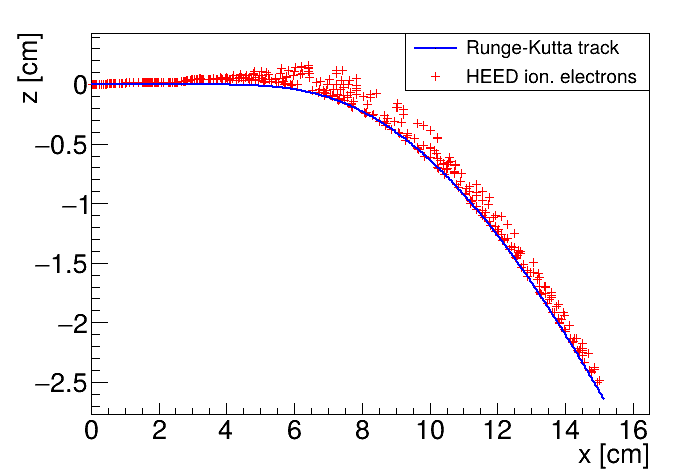
\includegraphics[width=0.48\textwidth]{rk_micro.png}
			\hfill
			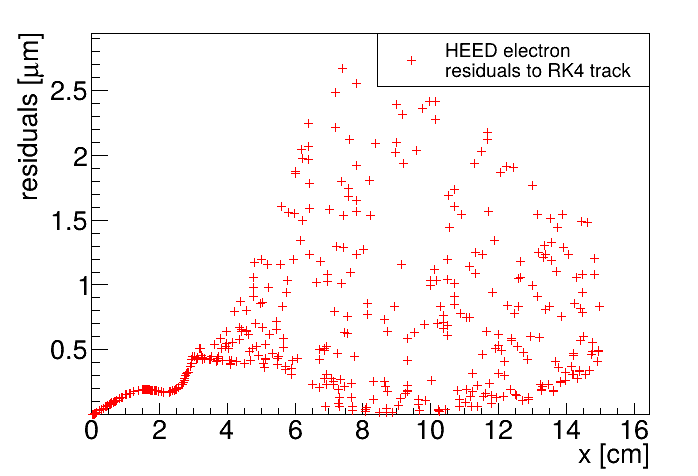
\includegraphics[width=0.48\textwidth]{rk_micro_res.png}
			\caption{A comparison of the \ac{HEED} track from the microscopic simulation in Section~\ref{sec:microfirst} with a~Runge-Kutta track with the same initial parameters and $\tau_\text{step} = 0.1$~ps (reducing the step further doesn't make a visible difference). In the view of the tracks on the left, the distance of the \ac{HEED} ionization electrons from the \ac{RK4} track is exaggerated $1000\cross$. On the right, the dependence of the \ac{HEED} electrons residuals (i.e., their shortest distance to the \ac{RK4} track) on their $z$\protect\nobreakdash-coordinate is shown.\red{~The images look the same even for 100,000x smaller step, so the residuals are a result of something that HEED does (maybe a different interpolation technique for the magnetic field? the pattern looks similar for two different tracks so it can't be scattering).}}
			\caption*{\footnotesize{When exaggerating, the \ac{HEED} ionization electrons are moved away along the shortest line connecting them to the \ac{RK4} track. The computation of this distance is described in Section~\ref{sec:rkfit}.}}
			\label{fig:rkmicro}
		\end{figure}
		
		\begin{figure}
			\centering
			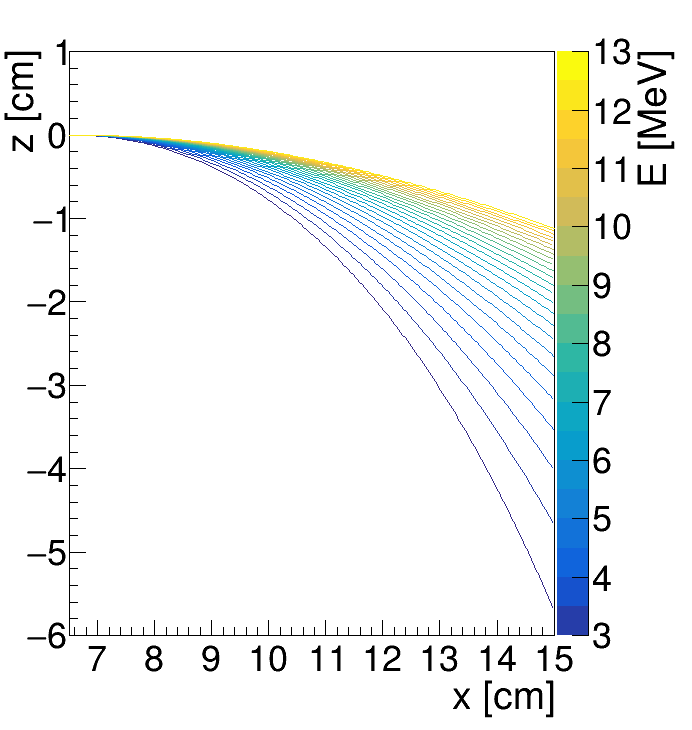
\includegraphics[width=0.7\textwidth]{rk_forward.png}
			\caption{Set of \num{25} Runge-Kutta tracks with initial position $(6.51,0,0)\,\unit{\cm}$, orientation $(1,0,0)$, and energies $\qtyrange{3}{13}{\MeV}$.}
			\label{fig:rk_forward}
		\end{figure}
					
		\subsection{Testing sample}
		\label{sec:rktest}		
		In order to test the simulation and reconstruction, a~sample of \num{1000000} tracks with randomized parameters (using \texttt{TRandom3} from ROOT) was generated:
		\begin{itemize}[topsep=4pt,itemsep=2pt]
			\item the Runge-Kutta step was set to \qty{1.67}{\ps} (coordinate time, each proper time step is adjusted by the gamma factor once at the beginning; for an \qty{8}{\MeV} track, $\tau_\text{step} = \qty{0.1}{\ps}$),
			\item the kinetic energy of the particle $E_\text{kin} = \qtyrange{3}{13}{\MeV}$,
			\item the starting point of the track is a~random point in the \ac{OFTPC} window,
			\item the initial direction is given by the line connecting a~random point on the target\footnote{To generate a~random point on the target, we generate a~random angle $\alpha$ and a~random square of the distance from origin $r^2$ to get a~uniform distribution.} (a~disc with 1~mm radius in the YZ plane).
		\end{itemize}
		Since the Runge-Kutta simulation is quite fast\footnote{One track with $t_\text{step} = \qty{1.67}{\ps}$ takes less than one millisecond to simulate.}, it can be run locally on any computer.
	\chapter{Track Reconstruction}
\label{sec:track}
	The~first stage of our reconstruction algorithm is the~reconstruction of the~track of the~primary particle (either an~electron or a~positron). The~results of this step are then used to determine the~energy of the~particle (see Section~\ref{sec:energy}).
	
	\textbf{First Attempts} at a~track reconstruction were made using the~standard approach. Here, we assume that the~readout coordinates ($x'$,~$y'$,~$t$) are known exactly, neglecting the~pads and time bins. In a~standard \ac{TPC} (with parallel fields), we only need to reconstruct the~$z$~coordinate from drift time using the~known drift velocity.
	
	Reconstruction using the~\textbf{Ionization Electron Map} (from now on referred to as \emph{the~map}) uses a~simulation of the~drift of secondary (ionization) electrons within the~detector volume. This simulation can then be used to interpolate the~initial position of the~secondary electrons. First attempts neglect the~pads.
	
	We used the~map for reconstruction in two different ways. The~first one uses gradient descent search along with trilinear interpolation (see Section~\ref{sec:trilin}) in the~map. The~second method uses interpolation in the~irregular inverse grid with a~linear polynomial.
	
	The~\textbf{Discrete Reconstruction} uses the~map; instead of reconstructing the~exact position of each electron, we reconstruct the~center of each hit pad with the~time corresponding to the~midpoint of the~time bin. The~number of electrons in each \ac{TPC}~bin (consisting of the~pad and the~time bin) is counted and used as a~charge in the~energy reconstruction.
	
	\section{First Attempts}
	\label{sec:trackfirst}
		As the~first step, we decided to try to reconstruct an~electron track with a~special set of initial parameters. The~origin of the~particle is given by the~origin of our coordinate system. The~initial direction is given by the~positive $x$~axis. This means the~magnetic field of our detector is perpendicular to the~momentum of our particle at all times, and we can reduce the~problem to two-dimensional space. We use a~track simulated using the~microscopic simulation (see Section~\ref{sec:microsim}) with a~kinetic energy of 8~MeV. The~gas composition used in this simulation is 90\%~Ar~+~10\%~CO$_2$.
		
		In this first approach to the~reconstruction of the~track, we decided to use the~common method used in a~standard \ac{TPC}. This will allow us to explore the~significance of the~atypical behavior in our \ac{OFTPC}. Additionally, we assume the~readout is continuous to further simplify the~problem. In this approximation, we reconstruct the~initial position of each ionization electron.
		
		The~reconstruction is then defined by the~following relations between the~coordinates of the~detector space and the~readout space (see Section~\ref{sec:coor}):
			\begin{eqnarray}
				x = x',\\
				y = y',\\
				z = v_d t,
			\end{eqnarray}
		where $v_d$ is the~drift velocity of electrons in the~given gas mixture. At a~phenomenological level, this velocity can be considered a~function of the~electric field~$\bm{E}$ and the~magnetic field~$\bm{B}$:
			\begin{equation}
				v_d = v_d(\bm{E},\bm{B}).
			\end{equation}
		\textcolor{red}{Taken from Garfield user manual.} The~Garfield++ toolkit uses this fact to accelerate their drift simulation with non-microscopic approaches. Since we assume a~uniform electric field in our detector and we want to neglect the~effect of our unusual magnetic field, we consider the~drift velocity to be constant in this scenario. We then approximate this velocity by fitting the~dependence $z(t)$ taken from the~simulated ionization electrons. \textcolor{red}{This is in one of the~provisional figures. Also, this description is not completely accurate; in reality, we fit t1:8-y0 with a1*x+a0 and then invert this and use 8-y0 = b1*t1+b0 (old coordinates); b1=1/a1 functions as the~drift velocity. Maybe also define this 8-z variable as an~alternative to z in Section~\ref{sec:coor} and then use it when correcting this.}
		
		\textcolor{red}{Later, in a~commit after this, I plotted some residues (provisional figure), which could be useful, but for some reason they are residuals from a~spline fit of the~track?! Probably redo this without the~spline fit; just explore the~difference in individual points.}
		
		\begin{figure}
			\centering
			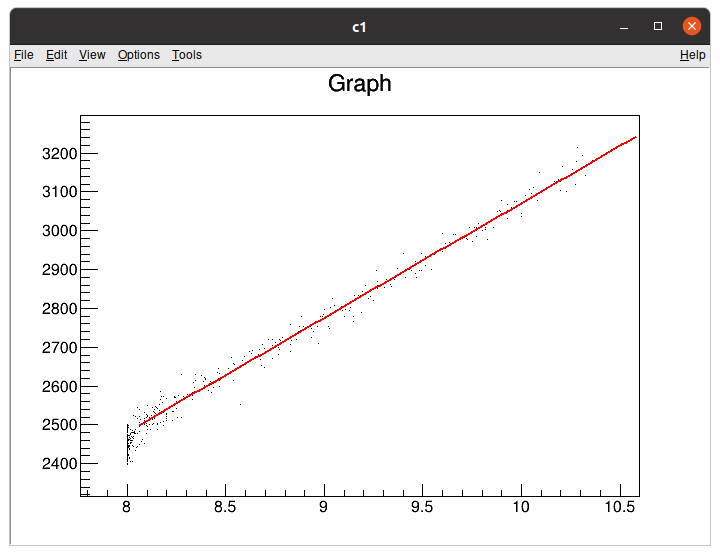
\includegraphics[width=0.5\textwidth]{9010_zt.png}
			\caption{Dependence of the~drift time on the~$z$~coordinate in 90~\%~argon and 10~\%~CO$_2$ atmosphere, fitted with a~linear function. The~fitted function gives us the~average drift velocity in the~gas and can be used for rough reconstruction in our \ac{TPC}. \textcolor{red}{Swap for better image with axis labels, etc. Maybe write the~fitted equation.}}
			\label{fig:9010zt}
		\end{figure}
		
		\begin{figure}
			\centering
			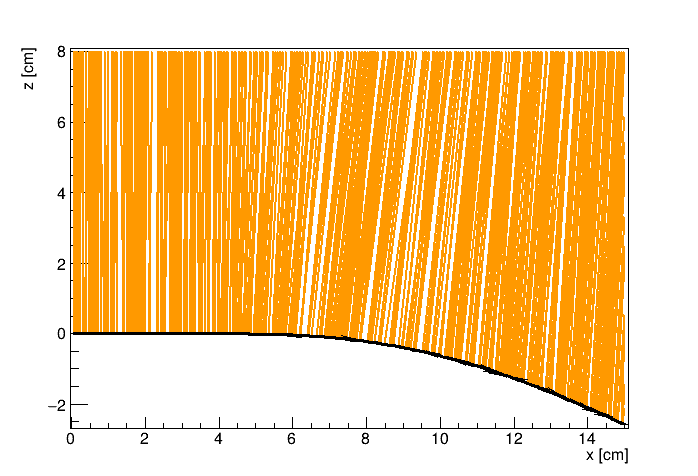
\includegraphics[width=0.5\textwidth]{9010_xz.png}
			\caption{First attempt at a~track reconstruction using only the~drift velocity. This approach works well in a~standard \ac{TPC} (\textcolor{red}{ideally cite some source?}). 90~\%~argon and 10~\%~CO$_2$ atmosphere. \textcolor{red}{Swap for better image, correct coordinates.}}
			\label{fig:9010xz}
		\end{figure}
		
		\begin{figure}
			\centering
			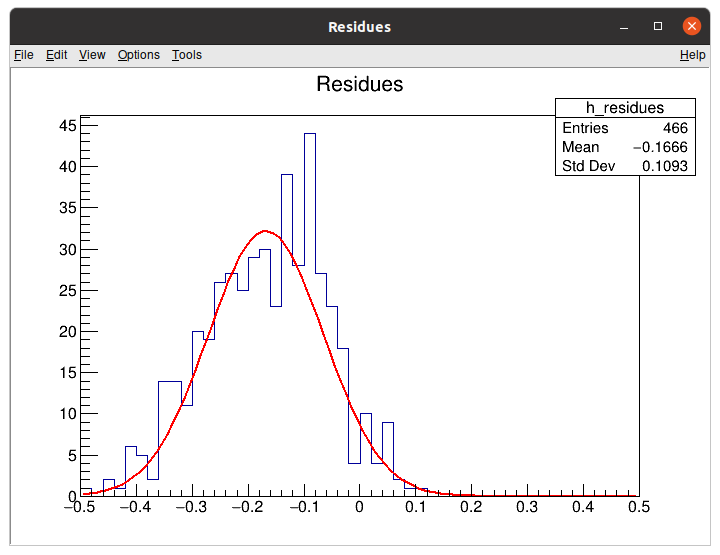
\includegraphics[width=0.5\textwidth]{9010_res.png}
			\caption{First attempt at a~track reconstruction using only the~drift velocity, residues. \textcolor{red}{Swap for better image, correct coordinates. What's causing the~shift? Explain details.}}
			\label{fig:9010res}
		\end{figure}
	
	\section{Ionization Electron Map}
	\label{sec:map}
		Inside an~\ac{OFTPC}, the~drift of the~secondary (ionization) electrons is significantly affected by its magnetic field. We need to take this into account for accurate reconstruction. In the~first approximation, we assume a~continuous readout (i.e., we neglect pads). We can then reconstruct the~original position of each ionization electron using its readout coordinates. For this purpose, we use the~ionization electron map.
		
		The~ionization electron map is a~mapping from the~detector space to the~readout space. It tells us what readout coordinates $(x',y',t)$ we can expect on average for an~ionization electron created in the~detector coordinates $(x,y,z)$. \textcolor{red}{More precisely it is a~mapping to the~distributions on the~readout space; we can simplify this as only the means $\overbar{\mathcal{M}}$ and the covariance matrices $\mathcal{M}_\text{cov}$, assuming Gaussian distribution.}
			\begin{equation}
				\mathcal{M}: \mathcal{D} \longrightarrow \mathcal{R},\; (x,y,z) \longmapsto (x',y',t).
			\end{equation}
		To get an~approximation of this mapping, we simulate the~drift of ionization electrons generated on a~regular grid inside the~volume of our \ac{OFTPC} (\textcolor{red}{actually, we don't take the~detector walls into account and simulate even outside of the~\ac{OFTPC}}). It is also useful to simulate multiple (100 in our case) electrons originating from the~same position so we can get a~better approximation of the~average drift and its variance. In order to get accurate results, we use the~microscopic simulation of these electrons described in Section~\ref{sec:microsim}. When evaluating the~map inside the~grid, we use trilinear interpolation (see Section~\ref{sec:trilin}). From now on, we will denote this interpolated simulation with the~same symbol $\mathcal{M}$.
		
		Finally, we need to invert the~map to get the~original detector coordinates $(x,y,z)$ for the~given readout coordinates $(x',y',t)$. \textcolor{red}{Two ways of inverting.}
		
		The~simulation of the~map is a~computationally heavy task. For this reason, we use a~grid MetaCentrum \textcolor{red}{(citation)} to parallelize it. At first, this was done by evenly distributing the~simulated electrons across the~individual jobs. This was used in the~first simulation with only one electron per vertex in the~regular grid with the~spacing of one centimeter. 
		
		Later, a~better approach was implemented, accounting for the~varying lengths of the~drift of individual electrons. If we index the~electrons in the~order of increasing coordinates $y,x,z$ (\textcolor{red}{picture?}), we can express the~number~$n_l$ of full XY~layers (i.e., electrons with the~same $z$~coordinate) of electrons with index less than or equal to $i$
			\begin{equation}
				n_l(i) = \left\lfloor\frac{i}{n_{xy}}\right\rfloor,
			\end{equation}
		where $n_{xy}$ is the~number of electrons in each XY~layer calculated simply by counting the~electrons that satisfy boundary conditions for $x$~and~$y$. \textcolor{red}{These conditions should be mentioned above; sector condition + maximal $x$ value.} The~number of electrons remaining in the~top layer is then
			\begin{equation}
				n_r(i) = i\!\!\!\!\mod n_{xy}.
			\end{equation}
		Finally, we can calculate the~sum of the~drift gaps of electrons up to index~$i$
			\begin{equation}
				d_\text{sum} = (z_\text{max}-z_\text{min})n_{xy}n_l-\frac{n_l(n_l-1)}{2}n_{xy}l+n_r(z_\text{max}-z_\text{min}-n_l l).
			\end{equation}
		We then use a~binary search algorithm to find the~maximum index $i$ such that the value of this sum is less than the~fraction $\frac{\text{job id}}{\text{max job id}}$ of the~total sum. This way we obtain the~minimal and the~maximal index of electrons simulated in the~given job.
		\textcolor{red}{The~spacing $l$ should be probably defined above + picture of the~simulating grid (1 layer). zmin zmax also}
		
		\textcolor{red}{After the~simulation of the~map, we calculate the~mean readout coordinates assuming Gaussian distribution (i.e., we use averages). We also calculate standard deviations in a~later commit, should be upgraded to the~covariance matrix. We never actually plotted the~distributions we get when simulating the~same electron multiple times, so we don't know if our assumptions are accurate (could also run some statistical test to see how well the~Gaussian distribution fits).}
		
		\textcolor{red}{The~map is then stored in a~\textit{Field}, a~custom class template, could expand on that. Maybe earlier, since the~same template is used for the~magnetic field.}
		
		\textcolor{red}{Could insert a~table here describing all 4 simulations of the~map (gas composition, spacing, etc.). Simulation inside one sector (at first double angle). Extra space on the~sensor. Edge cases not taken into account (TPC wall). Using qsub (not sure if important).}
		
		\textcolor{red}{Explanation of the~map, pictures. Simulated on MetaCentrum, workload distribution between multiple jobs. More electrons at one location to get statistics. There are two methods of reconstruction using this map. Comparison of 90/10 and 70/30 maps.}
		
		\begin{figure}
			\centering
			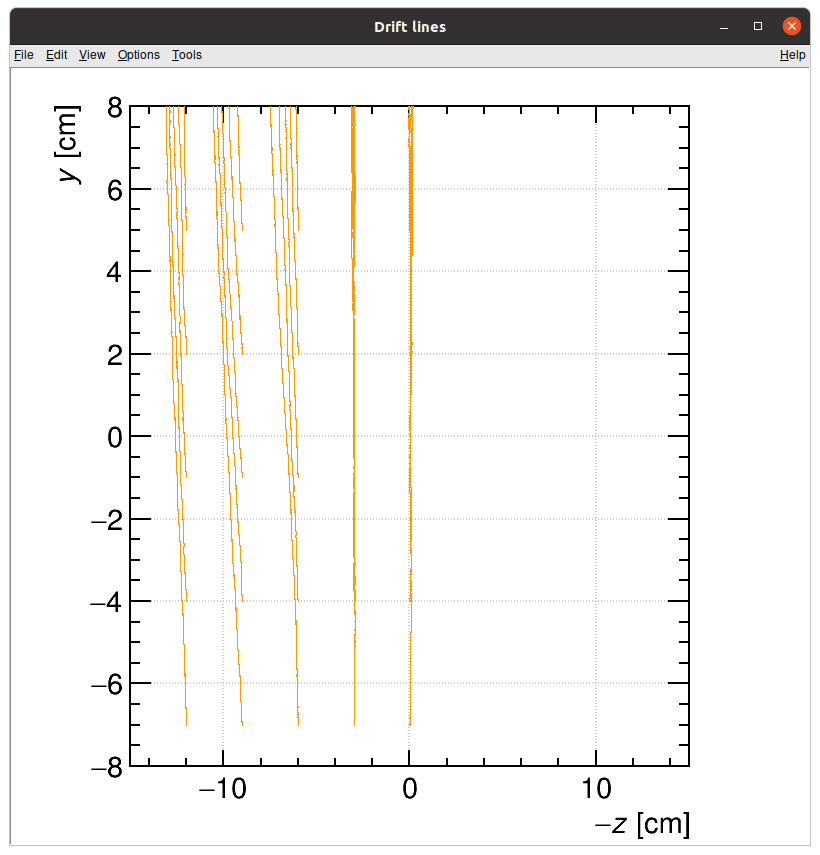
\includegraphics[width=0.5\textwidth]{map_9010_gen.png}
			\caption{Example of map generation. \textcolor{red}{Swap for better image, correct coordinates.}}
			\label{fig:map9010gen}
		\end{figure}
		
		\begin{figure}
			\centering
			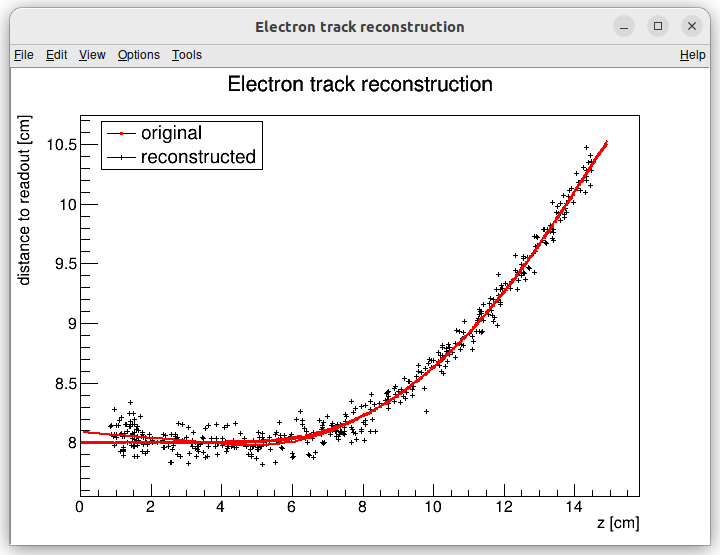
\includegraphics[width=0.5\textwidth]{9010_reco.png}
			\caption{Example reconstruction with the~map. \textcolor{red}{Swap for better image, correct coordinates.}}
			\label{fig:9010reco}
		\end{figure}
		
		\subsection{Gradient Descent Search}
			\label{sec:grad}
			\textcolor{red}{Gradient descent search of a~point in the~original space that gets mapped to the~given point of the~readout space (trilinear interpolation).}
			
			The~first implemented method of reconstruction uses a~gradient descent search to find an~approximation of the~point in detector space with given mean readout coordinates. Gradient descent is an~iterative minimization algorithm for multivariate functions. Let $R\in\mathcal{R}$ be a~point in the~readout space; we want to find a~point $D = (x,y,z) \in\mathcal{D}$ in the~detector space such that 
				\begin{equation}
					\overbar{\mathcal{M}}(D) = R = (x'_R,y'_R,t_R).
				\end{equation}
			We define a~function~$f_R$ in the~readout space as a~modified distance in this space:
				\begin{equation}
					f_R(x',y',t) = \sqrt{(x'-x'_R)^2+(y'-y'_R)^2+v_d^2(t-t_R)^2},
				\end{equation}
			where $v_d$ is an~approximation of the~drift velocity in the~\ac{TPC}, obtained from the~reconstruction in Section~\ref{sec:trackfirst} (\textcolor{red}{there will be an image with the~linear fit there}). We make the~initial guess (\textcolor{red}{actually in the~original code we just take $z=0$}):
				\begin{equation}
					D_0 = (x'_R,y'_R,v_dt).
				\end{equation}
			Assuming we have the $n$-th estimate $D_n$, we calculate an~approximation of the~$i$-th component of the~gradient of $f_R\circ\mathcal{M}$:
				\begin{equation}
					\nabla(f_R\circ\mathcal{M})^i \approx \frac{f_R(\mathcal{M}(D_n+s\cdot e^i))-f_R(\mathcal{M}(D_n-s\cdot e^i))}{2s},
				\end{equation}
			where $s$ is a~number and $e^i\in\mathcal{D}$ is the~$i$-th coordinate vector. The~number $s$ should be sufficiently small; initially, we set it as a~fraction of the~map's grid spacing $s = \frac{l}{10}$. During the~minimization, we check that $f_R(\mathcal{M}(D_n))<10s$ at all times. \textcolor{red}{When using trilinear interpolation, it would be more efficient to calculate the~gradient explicitly ($\pm$ same result). This could be implemented inside the~\textit{Field} template class.} The~next estimate can be calculated as follows:
				\begin{equation}
					D_{n+1} = D_n - \gamma \nabla(f_R\circ\mathcal{M})(D_n),
				\end{equation}
			where $\gamma\in\mathbb{R}^+$ is the~damping coefficient. It should be set to a~small enough value to ensure convergence, but large enough for sufficient converging speed. The~minimization stops either when the error $f_R(\mathcal{M}(D_n))$ drops below a~specified value or when the~number of iterations exceeds 1000 (in this case, a~message is printed into the~console).
			The parameters of this method could be further optimized (e.g., a~better choice of $\gamma$, \textcolor{red}{gradient computation}); instead, we later decided to use the~interpolation in the~inverse grid described in the~next section.
			
			\textcolor{red}{Measure reconstruction duration and compare it with the~inverse grid interpolation? Also compare the~result? Not sure if this has to be cited.}
		
		\subsection{Interpolating in the~Inverse Grid}
			\textcolor{red}{Interpolating between known points in the~readout space. Gaussian elimination, multivariate polynomial. Benefits compared to the~gradient descent search method (one-time computation for the~whole map is easy to achieve if needed).}
			
			\begin{figure}
				\centering
				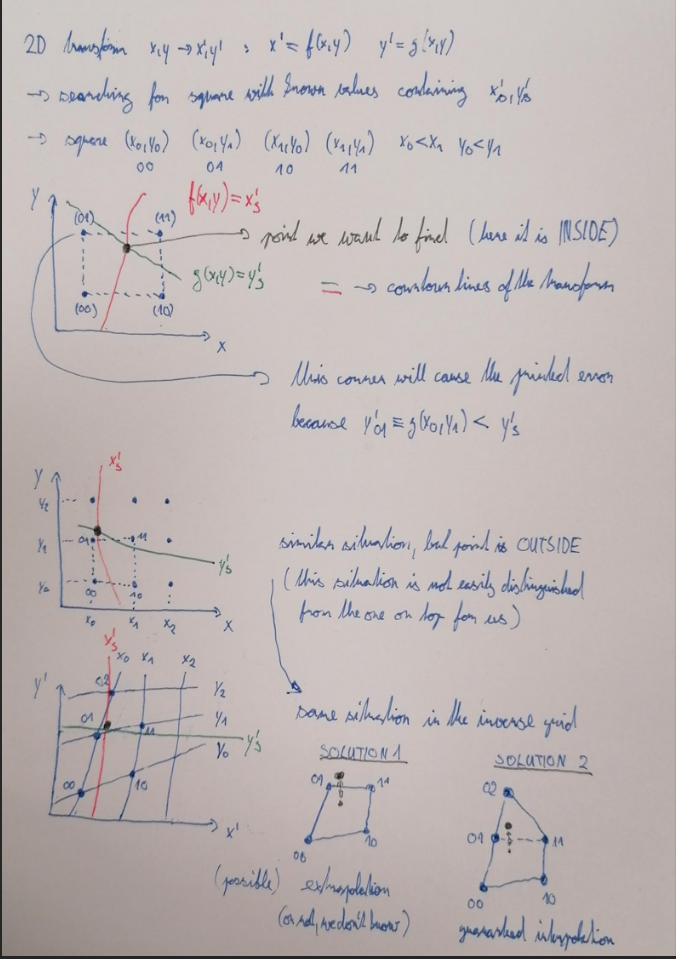
\includegraphics[width=0.8\textwidth]{interpol.png}
				\caption{Selection of the~points for interpolation. \textcolor{red}{Create better images; use the~explanation interpolation vs. extrapolation strange property. Solution~2 probably does not make much sense.}}
				\label{fig:interpol}
			\end{figure}
		
	\section{Discrete Reconstruction}
		\textcolor{red}{Reconstruction with pads and time bins. Maybe testing different pads. Mapping the~center of the pad (along with the~midpoint of the~time bin) isn't necessarily the~best approach since it might not correspond to the~average parameters of an~electron with these readout parameters (insignificant?).}
		
		\textcolor{red}{It is also possible to make this a~subsection of the~map, making the previous subsections parts of a~new subsection 'Map Inversion'.}
	\chapter{Energy Reconstruction}
\label{sec:energy}
	The~second stage is the reconstruction of the particle's energy using a~fit of its reconstructed track (see Section~\ref{sec:track}). We have tested three ways of reconstructing the energy. Fitting is done using the MINUIT algorithm implemented in ROOT~\cite{ROOT}.\red{~Cite some CERN article directly on MINUIT, can add a~section. Or is it done using MIGRAD? The circle and RK4 probably was.}
	
	The~\textbf{Cubic Spline Fit} was a~tested and later rejected method of energy reconstruction. It uses smoothly connected piecewise cubic polynomials between uniformly spaced nodes. The reconstructed energy is calculated using the fit parameters by computing the radius of curvature in different points of the fitted curve using the known magnitude of the magnetic field perpendicular to the trajectory. We rejected this method because the tuning of the fit turned out to be unpractical compared to the other used methods.\red{~Reconstructs energy at every position (even though the actual energy doesn't change much) and it might be slower but no profiling has been done yet. Of course, it wasn't tested on the newer track reconstruction methods at all.}
	
	The~\textbf{Circle and Lines Fit} was chosen as an~alternative since this corresponds to the shape of a~trajectory of a~charged particle crossing a~finite volume with a~homogeneous magnetic field. The~energy of the particle can be estimated using the fitted radius and the magnitude of the perpendicular magnetic field in the middle of the \ac{TPC}.
	
	The~\textbf{Runge-Kutta Fit} uses the 4th order Runge-Kutta numerical integration described in Section~\ref{sec:rks}. Initial parameters of the track (including the particle's energy) are optimized so that the integrated trajectory fits to the reconstructed one. This fit can also be performed as a~single parameter (i.e., energy) fit if we get the initial position and orientation of the particle on the entrance to the \ac{TPC} from previous detectors (\ac{TPX3} and \ac{MWPC}, see Section~\ref{sec:IEAP}).
	
	\section{Cubic Spline Fit}
	\label{sec:cspline}
		The~first method for the estimation of the kinetic energy of the particle uses a~cubic spline fit. We use an~electron track simulated using the microscopic simulation, described in detail in Section~\ref{sec:microfirst}. The track was reconstructed using the map described in Section~\ref{sec:map}.
				
		In order to calculate the spline, we use the class \textit{TSpline3} from ROOT. This allows us to evaluate the spline using the coordinates $(x_n,z_n)$ of each node and the derivatives $d_1,d_2$ in the first and the last node. We can fit these parameters of a~fixed amount of nodes to the simulated trajectory. We use the IMPROVE algorithm provided by the \textit{TMinuit} class in ROOT\orange{~(there are some guidelines for fonts in MFF UK template (Czech version) that I will eventually apply (see notes in the conclusion))}. This algorithm attempts to find a~better local minimum after converging\orange{~(could reformulate a~bit, taken word for word from some manual)}.
		
		After the fit converges, we calculate an~energy estimate using the radius of curvature, which we can extract from the fitted spline equation at every point of the trajectory. The~part of the spline corresponding to a~given node is defined as
			\begin{equation}
				z(x) = z_n + b \Delta x+c(\Delta x)^2+d(\Delta x)^3,
			\end{equation}
		where $\Delta x = x-x_n$ and $b,c,d$ are coefficients. Using this equation, we derive the radius of curvature\footnote{For the general formula see \url{https://en.wikipedia.org/wiki/Curvature\#Graph_of_a_function}.} as:
			\begin{equation}
				r(x) = \frac{\left(1+z'^2(x)\right)^\frac{3}{2}}{z''(x)} = \frac{\left(1+\left(b+2c\Delta x+3d(\Delta x)^2\right)^2\right)^\frac{3}{2}}{2c+6d\Delta x}.
			\end{equation}
		Based on the geometry of our~detector, we assume that the magnetic field satisfies $\bm{B}(x,0,z) = (0,B(x,z),0)$ for a~track in the XZ~plane. Since the electron is relativistic, the effect of the electric field on its trajectory is negligible. The~Lorentz force $F_L$ is then always perpendicular to the momentum of the electron and acts as a~centripetal force $F_c$\orange{~(not quite sure how to handle this then?)}:
			\begin{gather}
				\begin{aligned}
					\bm{F_L} &= \bm{F_c},\\
					\norm{e\bm{v}\times\bm{B}} &= \frac{\gamma m_e v^2}{r},\\
					e c\beta B &= \frac{E_{0e} \beta^2}{r\sqrt{1-\beta^2}},\\
					\sqrt{1-\beta^2} &= \frac{E_{0e} \beta}{ecBr},
				\end{aligned}\\
				\beta^2(x) = \left[1+\left(\frac{E_{0e}}{ecB(x,z(x))r(x)}\right)^2\right]^{-1}, \label{eq:ekin1}
			\end{gather}
		where $e$~is the elementary charge, $c$~is the speed of light in vacuum, $m_e$~is the rest mass of electron, $E_{0e} = m_e c^2$ is its rest energy, $\gamma$~is the Lorentz factor, $\bm{v}$~is the velocity of the electron, and $\beta = \frac{v}{c}$. The~kinetic energy for a~given point on the trajectory is then given as
			\begin{equation}
				\label{eq:ekin2}
				E_\text{kin}(x) = \left(\frac{1}{\sqrt{1-\beta^2(x)}}-1\right)E_{0e}.
			\end{equation}
		We could then average these estimates at multiple points (\red{possibly using some weights to account for the change in accuracy}) to get a~single value. An example of the~reconstruction for a~reconstructed track is shown in \cref{fig:spline}. This method was later rejected in favor of the circle and lines fit\orange{~(the name was already established at the beginning of the chapter)} described in the next section.
		
		\begin{figure}
			\centering
			\begin{subfigure}[t]{0.48\textwidth}
				\centering
				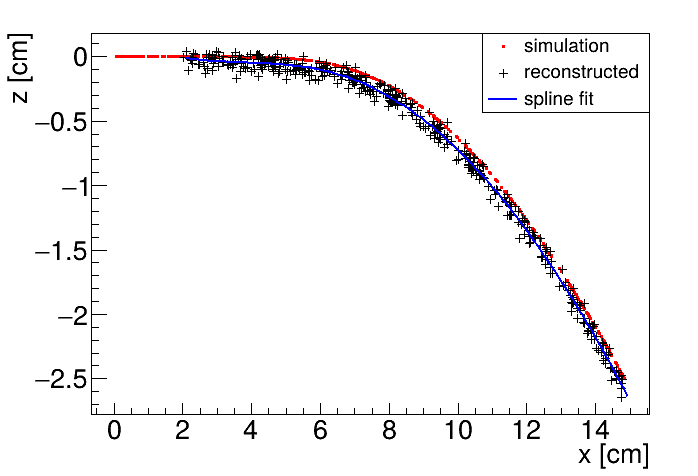
\includegraphics[width=\textwidth]{spline_fit.png}
				\caption{Spline fit of a~reconstructed track.}
			\end{subfigure}
			\hfill
			\begin{subfigure}[t]{0.48\textwidth}
				\centering
				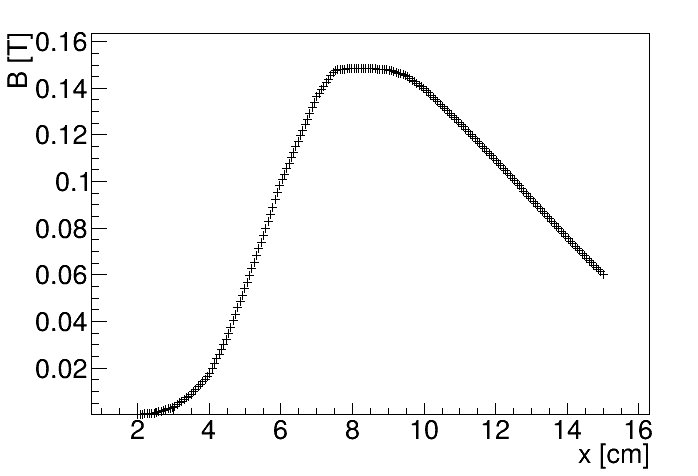
\includegraphics[width=\textwidth]{spline_mag.png}
				\caption{Magnetic field along the track.}
			\end{subfigure}
			\hfill
			\begin{subfigure}[t]{0.48\textwidth}
				\centering
				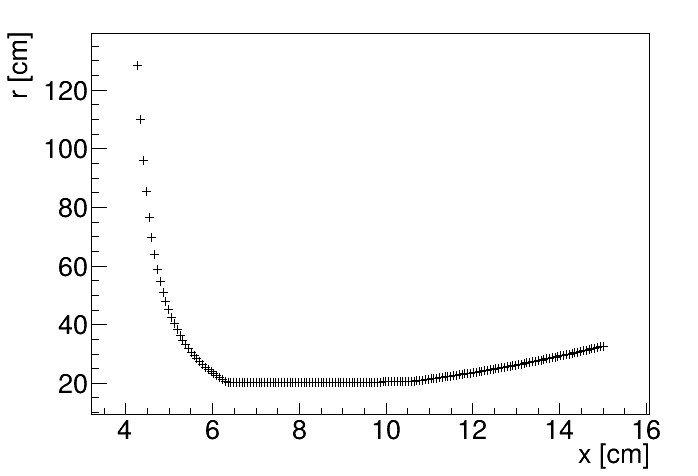
\includegraphics[width=\textwidth]{spline_radius.png}
				\caption{Reconstructed radius of curvature along the track.}
			\end{subfigure}
			\hfill
			\begin{subfigure}[t]{0.48\textwidth}
				\centering
				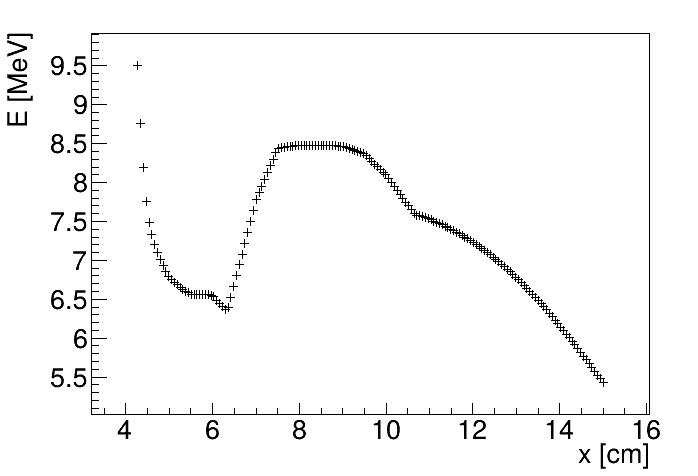
\includegraphics[width=\textwidth]{spline_energy.png}
				\caption{Reconstructed energy along the track.}
			\end{subfigure}
			\caption{Energy reconstruction of a~\qty{7.51}{\MeV} track in a~70:30 Ar:CO$_2$ gas mixture (described in detail in \cref{sec:microfirst}) using a~cubic spline fit with four evenly spaced nodes of points reconstructed using the map.}
			\label{fig:spline}
		\end{figure}
	
	\section{Circle and Lines Fit}
	\label{sec:clines}
		Another way to estimate the particle's kinetic energy is to~fit its\orange{~(??)} trajectory with a~circular arc with lines attached smoothly. This shape of trajectory corresponds to a~movement of a~charged particle through a~homogeneous magnetic field perpendicular to the particle's momentum and limited to a~certain volume. In general, the shape of such a~trajectory with a~non-perpendicularly oriented momentum is a~spiral. In our case, the magnetic field is approximately toroidal and the particle motion is nearly perpendicular to it\red{~(verify, could add some magnetic field plots in different vertical planes; shouldn't have a big effect on the reconstructed radius anyway)}. At first, we tested a~2D version of this fit, then we adapted it to 3D.
		
		The~field in our detector is not homogeneous, it is therefore not entirely clear what value of magnetic field should be used along with the fitted radius (using equations~\ref{eq:ekin1} and~\ref{eq:ekin2}) to get the best estimate for the kinetic energy. Since we only use this method as the first iteration of the particle's energy that we later refine, an~optimal solution of this problem is not required. Instead, we tested two options: taking the value of the field in the middle of the fitted circular arc\red{~(or is it in the middle $x$ of the OFTPC?)} and taking the average field along it.\red{~We haven't really tried to plot this for multiple tracks, but these estimates are saved somewhere and could be plotted.}
		
		\subsection{Two-dimensional fit}
			In the 2D case, the fitted function used for the electron track\footnote{Electron tracks bend towards negative~$z$, we need to use the upper part of the circle.} described in Section~\ref{sec:microfirst}\red{~(one specific track at the time, technically this function doesn't work for a curvature that gets outside of the semicircle)} is defined as follows:
				\begin{equation}
					\label{eq:clines2d}
					z(x) = \begin{cases}
								a_1x+b_1 & x<x_1\\
								z_0+\sqrt{r^2-(x-x_0)^2} & x_1\leq x\leq x_2\\
								a_2x+b_2 & x>x_2
						   \end{cases},
				\end{equation}
			where $a_{1,2}$ and $b_{1,2}$ are the parameters of the lines, $(x_0,z_0)$ is the center of the circle, $r$ is its radius, and $(x_{1,2},z_{1,2})$ are the coordinates of the function's nodes. That means we have 9~parameters ($z_{1,2}$ are not used in the function) along with 2~continuity conditions and 2~smoothness conditions\orange{~(9~parameters of the described function, 5~of them independent after taking the conditions into account)}. For the fit, we use the coordinates of the nodes and the radius of the circle, which gives us 5~independent parameters (only the radius has to be larger than half of the distance between nodes). The~continuity conditions (combined with the relations for $z_{1,2}$) are
				\begin{equation}
					\label{eq:ccont}
					z_{1,2} = a_{1,2}x_{1,2}+b_{1,2} = z_0-\sqrt{r^2-(x_{1,2}-x_0)^2},
				\end{equation}
			the smoothness conditions are
				\begin{equation}
					\label{eq:a12}
					a_{1,2} = \frac{x_0-x_{1,2}}{\sqrt{r^2-(x_{1,2}-x_0)^2}}.
				\end{equation}
			Together with the Equation~\ref{eq:ccont} we get the values of $b_{1,2}$
				\begin{equation}
					\label{eq:b12}
					b_{1,2} = z_{1,2} - a_{1,2} x_{1,2}.
				\end{equation}
			For the coordinates of the center of the circle, we can use the fact that the center has to lie on the axis of its chord. In other words, there is a~value of a~parameter~$t$ such that, using the parametric equation of the axis
				\begin{equation}
					\begin{pmatrix} x_0\\ z_0 \end{pmatrix} = \begin{pmatrix} \frac{x_1+x_2}{2}\\ \frac{z_1+z_2}{2} \end{pmatrix} + t \begin{pmatrix} \frac{z_2-z_1}{2}\\ \frac{x_1-x_2}{2} \end{pmatrix}.
				\end{equation}
			At the same time, the center has to be in a~distance of $r$ from the nodes:
				\begin{gather}
					(x_1-x_0)^2 + (z_1-z_0)^2 = r^2,\notag\\
					\left(\frac{x_1-x_2}{2}+\frac{z_1-z_2}{2}t\right)^2 + \left(\frac{z_1-z_2}{2}+\frac{x_2-x_1}{2}t\right)^2 = r^2,\notag\\
					\left(\left(\frac{x_2-x_1}{2}\right)^2+\left(\frac{z_2-z_1}{2}\right)^2\right)t^2+\left(\frac{x_2-x_1}{2}\right)^2+\left(\frac{z_2-z_1}{2}\right)^2-r^2=0.
				\end{gather}
			Since our electron track bends towards negative $z$ and $x_2 > x_1$, we only care about the solution with $t>0$
				\begin{gather}
					t = \sqrt{\frac{r^2}{\left(\frac{x_2-x_1}{2}\right)^2+\left(\frac{z_2-z_1}{2}\right)^2}-1},\\
					\begin{aligned}
						x_0 = \frac{x_1+x_2}{2} + \frac{z_2-z_1}{2} \sqrt{\frac{r^2}{\left(\frac{x_2-x_1}{2}\right)^2+\left(\frac{z_2-z_1}{2}\right)^2}-1},\label{eq:xz0}\\
						z_0 = \frac{z_1+z_2}{2} - \frac{x_2-x_1}{2} \sqrt{\frac{r^2}{\left(\frac{x_2-x_1}{2}\right)^2+\left(\frac{z_2-z_1}{2}\right)^2}-1}.
					\end{aligned}
				\end{gather}
			The~function defined in Equation~\ref{eq:clines2d} along with equations~\ref{eq:a12}, \ref{eq:b12}, and \ref{eq:xz0} derived using the continuity and smoothness conditions (combined with the relations for $z_{1,2}$) fully define our fitted function with parameters $r,x_{1,2},z_{1,2}$.
			
			For the calculation of kinetic energy from the radius of the circle, we use the value of the magnetic field in the middle of the \ac{OFTPC}\red{~(this could be further optimized in the future)}. An example of a~fit of vertices reconstructed with the map is shown in \cref{fig:circle2d}.\red{~Use GeoGebra schematics to generate a~picture of 2D geometry.}
			
			\begin{figure}
				\centering
				\includegraphics[width=0.48\textwidth]{circ2d_fit.png}
				\hfill
				\includegraphics[width=0.48\textwidth]{circ2d_mag.png}
				\caption{Circle and lines 2D energy reconstruction of a \qty{7.51}{\MeV} track in a~70:30 Ar:CO$_2$ gas mixture (described in detail in \cref{sec:microfirst}). The resulting energy is \qty{7.70}{\MeV}, the magnetic field along the track is shown on the right.}
				\label{fig:circle2d}
			\end{figure}
		
		\subsection{Three-dimensional fit}
			In three dimensions, the shape of a~trajectory of a~charged particle in a~uniform magnetic field is a~cylindrical helix. Nevertheless, since we assume that the field is approximately perpendicular to the particle's momentum at all times, we will further approximate the trajectory with a~circular arc $\mathbf{X}_\text{C}(\phi)$ (with lines $\mathbf{X}_\text{L1}(t),\mathbf{X}_\text{L2}(s)$ attached smoothly).
			
			We assume that the initial position $\mathbf{X}_0 = (x_0,y_0,z_0)$ and direction $\theta,\varphi$\red{~(spherical angles as in Section~\ref{sec:coor})} are known, since this information will be provided by \ac{TPX3} and \ac{MWPC} layers.\red{~We could further refine it at the end of the current algorithm with some kind of global fit (all detector layers).} The fit then has four free parameters (see \cref{fig:circle3d}):
				\begin{itemize}[nosep]
					\item the length of the first line $l$ (as measured from the initial position),
					\item the radius of the circular arc $r$,
					\item the central angle of the arc $\phi_\text{max} \in [0,2\pi]$,
					\item the direction of the curvature given by the angle $\alpha \in [0,2\pi]$ (right-handed with respect to the particle direction, $\alpha = 0$ if the particle curves towards negative~$z$ in a~plane given by~$\hat{z}$ and the direction vector).
				\end{itemize}
			\begin{figure}
				\centering
				\includegraphics[width=0.8\textwidth]{circle3d.png}
				\caption{Visualization of the 3D geometry of the Circle and Lines Fit and its parameters.}
				\label{fig:circle3d}
			\end{figure}
			Using these parameters, we can derive a parametrization of the whole curve. Let $\mathbf{v}$ be the initial unit direction vector, i.e., using the spherical angles
				\begin{equation}
					\mathbf{v} = (\cos\varphi\cos\theta, \,\sin\varphi\cos\theta, \,\sin\theta)^\mathrm{T},
				\end{equation}
			then we can parameterize the first line as follows:
				\begin{equation}
					\mathbf{X}_\text{L1}(t) = \mathbf{X}_0 + t\mathbf{v} \quad t\in[0,l].
				\end{equation}
			This gives us the starting point of the arc
				\begin{equation}
					\mathbf{X}_1 = \mathbf{X}_\text{L1}(l) = \mathbf{X}_0 + l\mathbf{v}.
				\end{equation}
			The vector $\mathbf{c}_1$ that lies in the plane of curvature and points from $\mathbf{X}_1$ to the center of curvature can be calculated using a composition of rotations. First, we rotate $\mathbf{v}$ to point in the $\mathbf{\hat{x}}$ direction, the normal for $\alpha = 0$ than points in the $-\mathbf{\hat{z}}$ direction, we apply the $\alpha$ rotation and reverse the rotations into the $\mathbf{\hat{x}}$ direction:\orange{~(parameters are explained in the bullet points above)}
				\begin{equation}
					\begin{aligned}
						\mathbf{c}_1 &= R_z(\varphi)R_y(-\theta)R_x(\alpha)R_y\left(\frac{\pi}{2}\right)R_y(\theta)R_z(-\varphi)\mathbf{v},\\
						&= R_z(\varphi)R_y(-\theta)R_x(\alpha)(-\mathbf{\hat{z}}),\\
						&= \scalebox{0.95}{$
								\begin{pmatrix}
									\cos\varphi & -\sin\varphi & 0\\
									\sin\varphi & \cos\varphi & 0\\
									0 & 0 & 1
								\end{pmatrix}
								\begin{pmatrix}
									\cos\theta & 0 & -\sin\theta\\
									0 & 1 & 0\\
									\sin\theta & 0 & \cos\theta
								\end{pmatrix}
								\begin{pmatrix}
									1 & 0 & 0\\
									0 & \cos\alpha & -\sin\alpha\\
									0 & \sin\alpha & \cos\alpha
								\end{pmatrix}
								\begin{pmatrix}
									0\\ 0\\ -1
								\end{pmatrix}
							$},\\
						&= 	\begin{pmatrix}
								-\sin\alpha\sin\varphi+\cos\alpha\cos\varphi\sin\theta\\
								\phantom{-}\sin\alpha\cos\varphi+\cos\alpha\sin\varphi\sin\theta\\
								-\cos\alpha\cos\theta
							\end{pmatrix}.
					\end{aligned}
				\end{equation}
			\orange{Signs should be correct because right-handed rotation around $y$ rotates $z$ into $x$ and this one is the opposite.}\red{~Seems like in this part of the code $\theta$ is actually taken from the pole. Instead of the equator plane.} Similarly by rotating $\mathbf{\hat{y}}$, we can get the normal vector $\mathbf{n}=\mathbf{v}\cross\mathbf{c}_1$ perpendicular to the plane of the trajectory:
				\begin{equation}
					\mathbf{n} = R_z(\varphi)R_y(-\theta)R_x(\alpha)\mathbf{\hat{y}}=
									\begin{pmatrix}
										-\cos\alpha\sin\varphi-\sin\alpha\cos\varphi\sin\theta\\
										\phantom{-}\cos\alpha\cos\varphi-\sin\alpha\sin\varphi\sin\theta\\
										\sin\alpha\cos\theta
									\end{pmatrix}.
				\end{equation}
			This allows us to express the coordinates of the center $\mathbf{C}$ of the circular arc:
				\begin{equation}
					\mathbf{C} = \mathbf{X}_1+r\mathbf{c}_1.
				\end{equation}
			We can then get the parametrization and the endpoint of the circular arc using Rodrigues' rotation formula:\orange{~(all parameters explained in the bullet points above)}
				\begin{gather}
					\begin{aligned}
						\mathbf{c}_2 &= \mathbf{c}_1\cos\phi_\text{max} + (\mathbf{n}\cross\mathbf{c}_1)\sin\phi_\text{max} + \mathbf{n}(\mathbf{n}\cdot\mathbf{c}_1)(1-\cos\phi_\text{max}),\\
						&= \mathbf{c}_1\cos\phi_\text{max} - \mathbf{v}\sin\phi_\text{max},
					\end{aligned}\\
					\mathbf{X}_\text{C}(\phi) = \mathbf{C} - r(\mathbf{c}_1\cos\phi - \mathbf{v}\sin\phi) \quad \phi\in[0,\phi_\text{max}],\\
					\mathbf{X}_2 = \mathbf{X}_\text{C}(\phi_\text{max}) = \mathbf{C} - r\mathbf{c}_2,
				\end{gather}
			and if we define the direction vector of the second line, we also get its parametrization
				\begin{gather}
					\mathbf{w} = \mathbf{v}\cos\phi_\text{max} + (\mathbf{n}\cross\mathbf{v})\sin\phi_\text{max} = \mathbf{v}\cos\phi_\text{max} + \mathbf{c}_1\sin\phi_\text{max},\\
					\mathbf{X}_\text{L2}(s) = \mathbf{X}_2 + s\mathbf{w} \quad s\in[0,\infty).
				\end{gather}
				
			The fit is performed as a~(weighted) least square minimization\red{~(MIGRAD ROOT)}, therefore we need to derive the distance of any point~$\mathbf{P}$ to the fitted curve. For the first line, we simply compute the parameter value of the closest point on the line:
				\begin{equation}
					\label{eq:segdist}
					\begin{aligned}
						t_P &= \mathbf{v}\cdot(\mathbf{P}-\mathbf{X}_1),\\
						d_{P1} &= \norm{\mathbf{P}-\mathbf{X}_\text{L1}(t_P)}.
					\end{aligned}
				\end{equation}
			If the parameter value is outside of its bounds defined above, we take the boundary value instead. The distance to the second line is computed likewise. For the circular arc\orange{~(specific circular arc in the fit)}, we find the closest point\orange{~(on the arc)} by projecting the center connecting line onto the arc plane:
				\begin{gather}
					\mathbf{X}_{PC} = \mathbf{C} + r\frac{(\mathbf{P}-\mathbf{C})-(\mathbf{n}\cdot(\mathbf{P}-\mathbf{C}))\mathbf{n}}{\norm{(\mathbf{P}-\mathbf{C})-(\mathbf{n}\cdot(\mathbf{P}-\mathbf{C}))\mathbf{n}}},\\
					d_{PC} = \norm{\mathbf{P}-\mathbf{X}_{PC}}
				\end{gather}
			 If the point $\mathbf{X}_{PC}$ lies outside of the arc, distance to the closest endpoint is taken instead. The~shortest distance out of $d_{P1},d_{PC},d_{P2}$ is then taken as the distance to the curve.\red{~When calculating energy with the average field, only the arc is considered. Middle field in the current implementation taken in the middle~$x$ plane (intersection with the curve). TVirtualFitter+MIGRAD, maximal num of iterations, toleration. Different uncertainties in $x,y,z$ not taken into account.}
			
			\red{Fit details (parameter bounds, initial setting).}
			
			\subsection{Testing on a~Runge-Kutta sample}
				The~three dimensional circle and lines fit was tested on a~sample of Runge-Kutta tracks with randomized parameters described in Section~\ref{sec:rktest}. These tracks of primary electrons and positrons consist of points calculated with the \ac{RK4} algorithm for a~given proper time step\red{~(step can be adjusted by dividing by the gamma factor $\rightarrow$ detector time)}.\red{~Fitting with circle only was also partially implemented (didn't work but could be fixed/tuned).}
	
	\section{Runge-Kutta Fit}
	\label{sec:rkfit}
		The~Runge-Kutta fit uses the \acf{RK4} numerical integration of the equation of motion (see Section~\ref{sec:rks}) to find the best values of the track parameters -- the track origin, initial velocity direction and the kinetic energy. In order to speed up the energy reconstruction, an~initial guess of these parameters can be obtained from the 3D circle fit described in the previous section. Furthermore, assuming we know the track origin and orientation, we can perform a~single parameter fit of the kinetic energy\red{~(do some profiling and show that it is faster -- below in the microscopic testing)}.
		
		The~fit is performed as a~least square minimization of the (weighted) distances of the track points (true ionization vertices from the simulation or reconstructed points). The simulated \ac{RK4}~track consists of line segments with known endpoints, therefore we can calculate the distance of a~point from this segment analogically to Equation~\ref{eq:segdist} with $\mathbf{v}$ given as a~unit vector in the direction of the segment.
		
		We need to find the segment with the lowest distance. We assume, that the distance $d_\mathbf{P}(\tau)$ of a~point $\mathbf{P}$ to the point on the track (a~curve parameterized by the proper time $\tau$) $\mathbf{X}(\tau)$ has a~single minimum (local and global), no local maximum (except the interval endpoints) and no~saddle point
			\begin{equation}
				\label{eq:rk_assum}
				\exists!\tau_\text{min}\in[0,\tau_N]\colon\ \left(\forall\tau\in[0,\tau_N]\colon  d_{\mathbf{P}}(\tau) \geq d_{\mathbf{P}}(\tau_\text{min})\right)\ \lor\ \dv{d_{\mathbf{P}}}{\tau}{(\tau_\text{min})} = 0,
			\end{equation}
		where $N$ is the number of \ac{RK4} steps. This is a~reasonable assumption for a~track with an~approximate shape of a~circular arc with a~radius $r$, since the distance $d$ from a~point $\mathbf{C}$ on the corresponding circle of a~point $\mathbf{P}$ offset by~$a$ from the arc plane and by~$b$ from the arc's center when projected on its plane is given by the law of cosines:
			\begin{equation}
				\label{eq:rkdemo}
				d^2 = a^2+b^2+r^2 - 2br\cos\alpha,
			\end{equation}
		where $\alpha$ is the angle between points~$\mathbf{C}$ and~$\mathbf{P}$ as seen from the center of the arc (see \cref{fig:rkdemo}). This function is strictly convex for $\alpha\in\left(-\frac{\pi}{2},\frac{\pi}{2}\right)$ and in our case, the center of the arc lies outside of the detector and $\alpha$ is restricted to a~small interval around zero\red{~(especially considering that the initial guess should make the fitted trajectory reasonably close to any relevant point, in the worst-case scenario, the distance is overestimated which should keep the fit from converging to such solutions)}.
		
		\begin{figure}
			\centering
			\begin{subfigure}[t]{0.7\textwidth}
				\centering
				\includegraphics[width=\textwidth]{rk_circle_demo.png}
			\end{subfigure}
			\hfill
			\begin{subfigure}[t]{0.29\textwidth}
				\centering
				\includegraphics[width=\textwidth]{rk_circle_demo2.png}
			\end{subfigure}
			\caption{Demonstration of the convexity of the distance function $d(\alpha)$ for a~circular track (see Equation~\ref{eq:rkdemo}).}
			\label{fig:rkdemo}
		\end{figure}
		
		In a~more general case, if we consider the vector $\mathbf{a}(\tau) = \mathbf{P}-\mathbf{X}(\tau)$ whose size is $\norm{\mathbf{a}(\tau)} = d_\mathbf{P}(\tau)$, then the we get
			\begin{equation}
				2d_{\mathbf{P}}\dv{d_{\mathbf{P}}}{\tau}= \dv{d^2_{\mathbf{P}}}{\tau} = 2\mathbf{a}\cdot\dv{\mathbf{a}}{\tau} = -2\mathbf{a}\cdot\dv{\mathbf{X}}{\tau},
			\end{equation}
		therefore for the derivative of~$d_\mathbf{P}(\tau)$ to be zero, $\mathbf{a}(\tau)$ has to be perpendicular to the tangent of the track. In 3D, for a~given $\mathbf{X}(\tau)$, this condition restricts $\mathbf{P}$ to a~plane. This means that on a~curving track, for any two points $\mathbf{X}(\tau_1),\mathbf{X}(\tau_2)$ with non-parallel tangents, we can find a~point~$\mathbf{P}$ that has $\dv{d_{\mathbf{P}}}{\tau}{(\tau_1)} = \dv{d_{\mathbf{P}}}{\tau}{(\tau_2)} = 0$, which violates the assumption~\ref{eq:rk_assum}. If we have a~circle-and-lines track as described in the previous sections, such a~point has to lie outside of the circular sector given by the arc.
		
		For a~planar track $\mathbf{X}(\tau) = \left(X_1(\tau),X_2(\tau)\right)$, the envelope of all its normals is the evolute of the curve (i.e., the set of centers of all its osculating circles). If the track has a~monotonous tangent angle
			\begin{equation}
				\alpha(\tau) = \atan{\frac{\dv{X_2}{\tau}}{\dv{X_1}{\tau}}}
			\end{equation}
		with minimal and maximal $\alpha$ differing by less than~$\pi$ (i.e., the track changes direction by less than $180^\circ$), then all intersections of the track's normals must lie in an area bordered by the evolute and the normals at the beginning and the end of the curve (from their intersection with the evolute to their mutual intersection, see \cref{fig:rkdemo2,fig:rkdemo3}). Together, these three boundaries define a closed shape that will lie outside of the \ac{OFTPC} for a~typical track in our detector\footnote{The smallest anticipated radius of curvature is \qty{39}{\cm} for an electron or positron with a~kinetic energy \qty{3}{\MeV} in a~\qty{0.3}{\tesla} magnetic field. All points in the exclusion area must be farther from the track and therefore outside the \ac{OFTPC}.}.
			\begin{figure}
				\centering
				\includegraphics[width=0.55\textwidth]{rk_dist_demo.png}
				\hfill
				\includegraphics[width=0.42\textwidth]{rk_dist_demo2.png}
				\caption{An example track (red) with a~polygonal chain approximation (green, representing a~\ac{RK4} simulation). The distance of the point~$\mathbf{P}$ from the chain is found using a~binary search among the distances to the vertices $d_\mathbf{P}(\tau_i)$ (blue) and subsequently calculating the distance to segments neighboring the found vertex (thus finding the minimum of the function $d_\mathbf{P}'(\tau)$, function $d_\mathbf{P}(\tau)$ for the actual track is showed for reference). This approach works if the condition~\ref{eq:rk_assum} is satisfied, which is not the case for a~point from the green area bordered by the normals at endpoints and the evolute of the track (orange).}
				\label{fig:rkdemo2}
			\end{figure}
			\begin{figure}
				\centering
				\includegraphics[width=0.6\textwidth]{rk_dist_demo3.png}
				\caption{An exclusion area (green) of a~track (red) bordered by its evolute and the normals at endpoints (orange), where the assumption~\ref{eq:rk_assum} is violated. Unlike the track in \cref{fig:rkdemo2}, this track has a~minimal curvature point in the middle, corresponding to the cusp on its evolute.}
				\label{fig:rkdemo3}
			\end{figure}
		
		With the assumption~\ref{eq:rk_assum}, we can find the segment on the \ac{RK4} track with the lowest distance to a~given point~$\mathbf{P}$ using a~binary search algorithm. Let the distance of the point from the $n$\nobreakdash-th vertex %(resp. segment) 
		be~$d_{\mathbf{P},n} = d_{\mathbf{P}}(\tau_n)$%(resp.~$d_{\mathbf{P},n}'$). For every~$n$, there is a~$\tau_n'\in[\tau_{n-1},\tau_n]$ such that $d_{\mathbf{P}}(\tau_n') = d_{\mathbf{P},n}'$. Since~$d_{\mathbf{P}}(\tau)$ is a~continuous convex function and $\tau \in [0,\tau_N]$ for a~\ac{RK4} track with $N+1$~points, there is a~single minimum $d_{\textbf{P},\text{min}} = d_{\mathbf{P}}(\tau_\text{min})$ for some~$\tau_\text{min}\in[0,\tau_N]$%\in\{\tau_n'\}_{n=1}^N$.\footnote{the distance to two neighboring segments can be the same if the closest point is in their common vertex $\tau_n' = \tau_{n+1}'$}
		. Then the difference $\Delta d_{\mathbf{P},n} = d_{\mathbf{P},n}-d_{\mathbf{P},n-1}$ satisfies
			%\begin{equation}
			%	\begin{aligned}
			%		\Delta d_{\mathbf{P},n} &\leq 0\quad \forall n \in \{1,\ldots,k\},\\
			%		\Delta d_{\mathbf{P},n} &\geq 0\quad \forall n \in \{k+1,\ldots,N\}.
			%	\end{aligned}
			%\end{equation}
			\begin{equation}
				\begin{aligned}
					\Delta d_{\mathbf{P},n} &< 0\quad \forall n \text{ such that } \tau_n < \tau_\text{min},\\
					\Delta d_{\mathbf{P},n} &> 0\quad \forall n \text{ such that } \tau_{n-1} > \tau_\text{min}.
				\end{aligned}
			\end{equation}
		Therefore, we can search for the segment containing $d_{\textbf{P},\text{min}} = d_{\mathbf{P}}(\tau_\text{min})$ with binary search starting with $\Delta d_{\mathbf{P},1}$ and $\Delta d_{\mathbf{P},N}$, then calculate the difference $\Delta d_{\mathbf{P},m}$ for the middle index $m = \left\lfloor\frac{N+1}{2}\right\rfloor$. If $\Delta d_{\mathbf{P},m} > 0$\red{~(minor bug in the implementation -- if the value for the maximal index is negative, it shouldn't change anything)}, we can replace the higher index with~$m$, otherwise we replace the lower index. The~search stops when the difference between the minimal and maximal index is one.\red{~Would it be better if they were the same (maybe not)? Then the minimal value is $d_{\mathbf{P},n-1}$ or $d_{\mathbf{P},N}$ and we can take the minimum of the distances from the two segments connected to $n-1$. Currently taking the maximal index (and starting at $N-2$ maximal index $\leftrightarrow$ $N-1$\nobreakdash-th point), this should be equivalent, since either $\Delta d_{\mathbf{P},\text{max}} > 0$ (in the code is equivalent to max-1 here) or we are at $N-1$. The minimum of the two distances still taken.}
		
		\red{Same details with MIGRAD etc. as previously.}
		
		\subsection{Testing on a~microscopic sample}
			The Runge-Kutta fit together with the 3D circle-and-lines pre-fit was tested on a~sample of tracks simulated using the microscopic simulation described in Section~\ref{sec:microsim}. At first, few tracks with randomized initial parameters (same as the Runge-Kutta sample in Section~\ref{sec:rktest}) were generated for preliminary testing. Later, a~sample with a~grid-like distribution of track parameters was generated (see Section~\ref{sec:microgrid} for details).
			
			\red{Initial parameters of the HEED track (also should be in the first testing track). Initial parameters set in the circle fit (if electron set alpha one way, otherwise other way) and parameter bounds.}
	
	\chapwithtoc{Conclusion}
	\textcolor{red}{Here or at the~end of each section. Something about the~future of this work?}
	
	\section*{Notes}
		\textcolor{red}{General notes about the~thesis:}
		\begin{itemize}[topsep=4pt,itemsep=2pt]
			\item \textcolor{red}{Check that all of the~classes and other code are marked the~same way in the~text. I used italics somewhere, could use different font for this instead.}
			\item \textcolor{red}{Check unbreakable space in front of articles. Remove excessive article usage with proper nouns.}
			\item \textcolor{red}{Currently using margins for single-sided printing (bigger on the left side).}
			\item \textcolor{red}{Check that present tense is used}
			\item \textcolor{red}{American English quotation marks (") instead of British English (').}
			\item \textcolor{red}{Some of the overfull hbox warnings might change if duplex printing is used (they generate black rectangles on the~edge of the page), leaving them be for now}
			\item \textcolor{red}{Check nobreakdash usage}
			\item \textcolor{red}{Check capitalized references (e.g., Figure, Section, Equation)}
			\item \textcolor{red}{Check \textbackslash(...\textbackslash) math mode instead of \$...\$. (actually unlike \textbackslash[...\textbackslash] math mode, there is apparently no real benefit to this clumsy syntax)}
			\item \textcolor{red}{Use siunitx package to ensure correct formatting.}
			\item \textcolor{red}{Check other stuff that's written in the MFF UK template. Apparently it has since been updated and there are some differences (check for them).}
			\item \textcolor{red}{Check correct subscripts in equation (italics vs no italics)}\\
			\item \textcolor{red}{Consistent bold marking of points/vectors}
		\end{itemize}
		\textcolor{red}{Random notes:}
		\begin{itemize}[topsep=4pt,itemsep=2pt]
			\item \textcolor{red}{Terminology consistency -- ionization/primary/secondary electrons}
			\item \textcolor{red}{Consistent \ac{TPC} vs \ac{OFTPC} acronym usage in the text or individual chapters.}
			\item \textcolor{red}{Only electrons that start and end in the~sector closer than 0.5~cm are used for reconstruction (newest version).}
			\item \textcolor{red}{Attachment, Penning transfer and secondary ionization not considered in the~microscopic simulation.}
			\item \textcolor{red}{Suspicious artifacts of trilinear interpolation in Figure~\ref{fig:mag}.}
		\end{itemize}
		
	\section*{Future}
		\textcolor{red}{Things planned for the future:}
		\begin{itemize}[topsep=4pt,itemsep=2pt]
			\item \textcolor{red}{Testing the reconstruction algorithm by measuring real particles with a~known energy distribution.}
			\item \textcolor{red}{The~\textbf{Fast Simulation with Ionization Electron Map} is planned for the~future. It will use the~\ac{HEED} program~\cite{HEED} to simulate the~primary particle and the~Ionization Electron Map (see Section~\ref{sec:map}) to simulate the~drift of secondary electrons. It should be significantly faster than the~Microscopic Simulation but offer comparable precision since it will rely on an already simulated drift map. (Primary track simulated in HEED. Readout parameters by interpolating the map.	Diffusion from the map for randomization.)}
			\item \textcolor{red}{Account for GEM, delta electrons, ...}
			\item \textcolor{red}{Likelihood approach instead of least squares (if it improves the~reconstruction significantly), we should at least use a~better method than taking the~center of the~TPC bin.}
			\item \textcolor{red}{More detailed electric field simulation (if needed, GEM will have more complex field)}
		\end{itemize}
		
		\subsection*{Likelihood - inverse map}
			\textcolor{red}{If we wanted to further improve this procedure, taking into account the whole map $\mathcal{M}$, we could make an "inverse map" from $\mathcal{R}$ to distributions on $\mathcal{D}$. We could achieve this by taking the~normalized probability density of an~electron with initial coordinates $(x,y,z)$ having readout coordinates $(x',y',t)$. If we fix $(x',y',t)$, we get an~unnormalized probability density $f(x,y,z) = \mathcal{M}_{(x,y,z)}(x',y',t)$ (assuming that all initial coordinates are a~priori equally likely). This could potentially improve the~discrete reconstruction if we take the~mean value of this probability density across the pad and time bin}
				\begin{equation}
					\color{red}
					f_\text{pad, bin}(x,y,z) = \frac{1}{A_\text{pad} \Delta t_\text{bin}} \int_\text{pad, bin} \mathcal{M}_{(x,y,z)}(x',y',t) 	\text{d}x'\text{d}y'\text{d}t
				\end{equation}
			\textcolor{red}{and using it for a~likelihood fit instead of using least squares. This still assumes that all initial coordinates are equally likely which is clearly not the~case for a~primary particle track. In the future, we could even use the~fast track simulation with the~map (should be possible to make around 1000 tracks per minute per core with current settings), create a~big set of tracks with reasonable parameters and use these to get an~approximation of the probability distribution of the~detector response. Some approximations would be necessary when interpreting the~data to decrease the~degrees of freedom of this distribution (we would have to pick a set of parameters and assume that some of them are independent). This could give us an~idea about the~best achievable resolution (how significantly will the~detector response differ for a~given change in energy). If the~difference is significant, we could try to further improve the~likelihood fit.}
	
	%%% Bibliography
	%%% Bibliography (literature used as a source)
%%%
%%% We employ biblatex to construct the bibliography. It processes
%%% citations in the text (e.g., the \cite{...} macro) and looks up
%%% relevant entries in the bibliography.bib file.
%%%
%%% See also biblatex settings in thesis.tex.

%%% Generate the bibliography. Beware that if you cited no works,
%%% the empty list will be omitted completely.

% We let bibliography items stick out of the right margin a little
\def\bibfont{\hfuzz=2pt}

\printbibliography[heading=bibintoc]
\vspace{1em}
\noindent \textbf{Acknowledgments:}
\begin{itemize}[nosep]
	\item MetaCentrum grid: Computational resources were provided by the e-INFRA CZ project (ID:90254), supported by the Ministry of Education, Youth and Sports of the Czech Republic.
	\item \Cref{fig:oftpc,fig:trilin,fig:microgrid,fig:map_3d,fig:circle3d,fig:rkdemo,fig:rkdemo2,fig:rkdemo3} were made with GeoGebra®.
	\item This work was supported by the GAČR - Czech Science Foundation grant GA21-21801S.
\end{itemize}


%%% In case you prefer to write the bibliography manually (without biblatex),
%%% you can use the following. Please follow the ISO 690 standard and
%%% citation conventions of your field of research.

% \begin{thebibliography}{99}
	%
	% \bibitem{lamport94}
	%   {\sc Lamport,} Leslie.
	%   \emph{\LaTeX: A Document Preparation System}.
	%   2nd edition.
	%   Massachusetts: Addison Wesley, 1994.
	%   ISBN 0-201-52983-1.
	%
	% \end{thebibliography}
	
	%%% Figures used in the thesis (consider if this is needed)
	\listoffigures
	
	%%% Tables used in the thesis (consider if this is needed)
	%%% In mathematical theses, it could be better to move the list of tables to the beginning of the thesis.
	\listoftables
	
	%%% Abbreviations used in the thesis, if any, including their explanation
	%%% In mathematical theses, it could be better to move the list of abbreviations to the beginning of the thesis.
	
\chapwithtoc{List of Abbreviations}
\begin{acronym}
	\acro{ALPHA}{Antihydrogen Laser Physics Apparatus}
	\acro{BONuS12}{Barely Off-shell NeUtron Structure \qty{12}{\GeV}}
	\acro{GEM}{Gas Electron Multiplier}
	\acro{HEED}{High Energy Electro-Dynamics}
	\acro{IEAPCTU}[IEAP~CTU]{Institute of Experimental and Applied Physics, Czech Technical University in Prague}
	\acro{IPC}{Internal Pair Creation}
	%\acro{IPCC}{Internal Pair Conversion Correlation}
	\acro{EPC}{External Pair Creation}
	\acro{LArTPC}{Liquid Argon \ac{TPC}}
	\acro{Micromegas}{MICRO-MEsh GAseous Structure}
	\acro{MPGD}{Micro-Pattern Gaseous Detector}
	\acro{MWPC}{Multi-Wire Proportional Chamber}
	\acro{OFTPC}{Orthogonal Fields \acs{TPC}}
	\acro{PCB}{Printed Circuit Board}
	\acro{RICH}{Ring Imaging Cherenkov Counter}
	\acro{RK4}{Runge-Kutta 4th order}
	\acro{RPC}{Resistive Plate Chamber}
	\acro{RPWELL}{Resistive Plate WELL}
	\acro{rTPC}{radial-drift \ac{TPC}}
	\acro{THGEM}{THick \acs{GEM}}
	\acro{ToA}{time\protect\nobreakdash-of\protect\nobreakdash-arrival}
	\acro{ToT}{time\protect\nobreakdash-over\protect\nobreakdash-threshold}
	\acro{TPC}{Time Projection Chamber}
	\acro{TPX3}{Timepix3}
	\acro{uPIC}[\textmu-PIC]{Micro-Pixel Gas Chamber}
	\acro{uRWELL}[\textmu-RWELL]{Micro-RWELL}
\end{acronym}
	
	%%% Attachments to the bachelor thesis, if any. Each attachment must be
	%%% referred to at least once from the text of the thesis. Attachments
	%%% are numbered.
	%%%
	%%% The printed version should preferably contain attachments, which can be
	%%% read (additional tables and charts, supplementary text, examples of
	%%% program output, etc.). The electronic version is more suited for attachments
	%%% which will likely be used in an electronic form rather than read (program
	%%% source code, data files, interactive charts, etc.). Electronic attachments
	%%% should be uploaded to SIS and optionally also included in the thesis on a~CD/DVD.
	%%% Allowed file formats are specified in provision of the rector no. 72/2017.
	% \appendix
	%\chapter{Attachments}
	
	%\section{First Attachment}
	
	% \openright
\end{document}